\documentclass[twoside]{book}

% Packages required by doxygen
\usepackage{fixltx2e}
\usepackage{calc}
\usepackage{doxygen}
\usepackage[export]{adjustbox} % also loads graphicx
\usepackage{graphicx}
\usepackage[utf8]{inputenc}
\usepackage{makeidx}
\usepackage{multicol}
\usepackage{multirow}
\PassOptionsToPackage{warn}{textcomp}
\usepackage{textcomp}
\usepackage[nointegrals]{wasysym}
\usepackage[table]{xcolor}

% Font selection
\usepackage[T1]{fontenc}
\usepackage[scaled=.90]{helvet}
\usepackage{courier}
\usepackage{amssymb}
\usepackage{sectsty}
\renewcommand{\familydefault}{\sfdefault}
\allsectionsfont{%
  \fontseries{bc}\selectfont%
  \color{darkgray}%
}
\renewcommand{\DoxyLabelFont}{%
  \fontseries{bc}\selectfont%
  \color{darkgray}%
}
\newcommand{\+}{\discretionary{\mbox{\scriptsize$\hookleftarrow$}}{}{}}

% Page & text layout
\usepackage{geometry}
\geometry{%
  a4paper,%
  top=2.5cm,%
  bottom=2.5cm,%
  left=2.5cm,%
  right=2.5cm%
}
\tolerance=750
\hfuzz=15pt
\hbadness=750
\setlength{\emergencystretch}{15pt}
\setlength{\parindent}{0cm}
\setlength{\parskip}{3ex plus 2ex minus 2ex}
\makeatletter
\renewcommand{\paragraph}{%
  \@startsection{paragraph}{4}{0ex}{-1.0ex}{1.0ex}{%
    \normalfont\normalsize\bfseries\SS@parafont%
  }%
}
\renewcommand{\subparagraph}{%
  \@startsection{subparagraph}{5}{0ex}{-1.0ex}{1.0ex}{%
    \normalfont\normalsize\bfseries\SS@subparafont%
  }%
}
\makeatother

% Headers & footers
\usepackage{fancyhdr}
\pagestyle{fancyplain}
\fancyhead[LE]{\fancyplain{}{\bfseries\thepage}}
\fancyhead[CE]{\fancyplain{}{}}
\fancyhead[RE]{\fancyplain{}{\bfseries\leftmark}}
\fancyhead[LO]{\fancyplain{}{\bfseries\rightmark}}
\fancyhead[CO]{\fancyplain{}{}}
\fancyhead[RO]{\fancyplain{}{\bfseries\thepage}}
\fancyfoot[LE]{\fancyplain{}{}}
\fancyfoot[CE]{\fancyplain{}{}}
\fancyfoot[RE]{\fancyplain{}{\bfseries\scriptsize Generated by Doxygen }}
\fancyfoot[LO]{\fancyplain{}{\bfseries\scriptsize Generated by Doxygen }}
\fancyfoot[CO]{\fancyplain{}{}}
\fancyfoot[RO]{\fancyplain{}{}}
\renewcommand{\footrulewidth}{0.4pt}
\renewcommand{\chaptermark}[1]{%
  \markboth{#1}{}%
}
\renewcommand{\sectionmark}[1]{%
  \markright{\thesection\ #1}%
}

% Indices & bibliography
\usepackage{natbib}
\usepackage[titles]{tocloft}
\setcounter{tocdepth}{3}
\setcounter{secnumdepth}{5}
\makeindex

% Hyperlinks (required, but should be loaded last)
\usepackage{ifpdf}
\ifpdf
  \usepackage[pdftex,pagebackref=true]{hyperref}
\else
  \usepackage[ps2pdf,pagebackref=true]{hyperref}
\fi
\hypersetup{%
  colorlinks=true,%
  linkcolor=blue,%
  citecolor=blue,%
  unicode%
}

% Custom commands
\newcommand{\clearemptydoublepage}{%
  \newpage{\pagestyle{empty}\cleardoublepage}%
}

\usepackage{caption}
\captionsetup{labelsep=space,justification=centering,font={bf},singlelinecheck=off,skip=4pt,position=top}

%===== C O N T E N T S =====

\begin{document}

% Titlepage & ToC
\hypersetup{pageanchor=false,
             bookmarksnumbered=true,
             pdfencoding=unicode
            }
\pagenumbering{roman}
\begin{titlepage}
\vspace*{7cm}
\begin{center}%
{\Large Y\+D\+L\+I\+D\+AR S\+DK \\[1ex]\large V1.\+3.\+2 }\\
\vspace*{1cm}
{\large Generated by Doxygen 1.8.11}\\
\end{center}
\end{titlepage}
\clearemptydoublepage
\tableofcontents
\clearemptydoublepage
\pagenumbering{arabic}
\hypersetup{pageanchor=true}

%--- Begin generated contents ---
\chapter{Y\+D\+L\+I\+D\+AR S\+DK P\+A\+C\+K\+A\+GE V1.3.2}
\label{md__home_yang_tmp_sdk_README}
\hypertarget{md__home_yang_tmp_sdk_README}{}
S\+DK test application for Y\+D\+L\+I\+D\+AR

Visit E\+AI Website for more details about Y\+D\+L\+I\+D\+AR.

\section*{How to build Y\+D\+L\+I\+D\+AR S\+DK samples }

1) Clone this project to your computer folder 2) Clone this project to your computer folder 2) Running cmake to build ydlidar\+\_\+test

\section*{How to run Y\+D\+L\+I\+D\+AR S\+DK samples }

--\$ cd samples --\$ ./ydlidar\+\_\+test /dev/tty\+U\+S\+B0 230400 0

You should see Y\+D\+L\+I\+D\+AR\textquotesingle{}s scan result in the console

\section*{Upgrade Log }

2018-\/05-\/02 version\+:1.\+0.\+0

1.\+Output screen corrdinates.

Install required dependencies\+:

1.\+pip install pymouse 
\chapter{Namespace Index}
\section{Namespace List}
Here is a list of all documented namespaces with brief descriptions\+:\begin{DoxyCompactList}
\item\contentsline{section}{\hyperlink{namespaceserial}{serial} }{\pageref{namespaceserial}}{}
\end{DoxyCompactList}

\chapter{Class Index}
\section{Class List}
Here are the classes, structs, unions and interfaces with brief descriptions\+:\begin{DoxyCompactList}
\item\contentsline{section}{\hyperlink{structcmd__packet}{cmd\+\_\+packet} }{\pageref{structcmd__packet}}{}
\item\contentsline{section}{\hyperlink{class_c_yd_lidar}{C\+Yd\+Lidar} }{\pageref{class_c_yd_lidar}}{}
\item\contentsline{section}{\hyperlink{structdevice__health}{device\+\_\+health} }{\pageref{structdevice__health}}{}
\item\contentsline{section}{\hyperlink{structdevice__info}{device\+\_\+info} }{\pageref{structdevice__info}}{}
\item\contentsline{section}{\hyperlink{class_event}{Event} }{\pageref{class_event}}{}
\item\contentsline{section}{\hyperlink{structfunction__state}{function\+\_\+state} }{\pageref{structfunction__state}}{}
\item\contentsline{section}{\hyperlink{struct_laser_config}{Laser\+Config} \\*A struct for returning configuration from the Y\+D\+L\+I\+D\+AR }{\pageref{struct_laser_config}}{}
\item\contentsline{section}{\hyperlink{struct_laser_scan}{Laser\+Scan} }{\pageref{struct_laser_scan}}{}
\item\contentsline{section}{\hyperlink{structlidar__ans__header}{lidar\+\_\+ans\+\_\+header} }{\pageref{structlidar__ans__header}}{}
\item\contentsline{section}{\hyperlink{class_locker}{Locker} }{\pageref{class_locker}}{}
\item\contentsline{section}{\hyperlink{classserial_1_1_millisecond_timer}{serial\+::\+Millisecond\+Timer} }{\pageref{classserial_1_1_millisecond_timer}}{}
\item\contentsline{section}{\hyperlink{structnode__info}{node\+\_\+info} }{\pageref{structnode__info}}{}
\item\contentsline{section}{\hyperlink{structnode__package}{node\+\_\+package} }{\pageref{structnode__package}}{}
\item\contentsline{section}{\hyperlink{structnode__packages}{node\+\_\+packages} }{\pageref{structnode__packages}}{}
\item\contentsline{section}{\hyperlink{struct_package_node}{Package\+Node} }{\pageref{struct_package_node}}{}
\item\contentsline{section}{\hyperlink{structserial_1_1_port_info}{serial\+::\+Port\+Info} }{\pageref{structserial_1_1_port_info}}{}
\item\contentsline{section}{\hyperlink{structsampling__rate}{sampling\+\_\+rate} }{\pageref{structsampling__rate}}{}
\item\contentsline{section}{\hyperlink{structscan__exposure}{scan\+\_\+exposure} }{\pageref{structscan__exposure}}{}
\item\contentsline{section}{\hyperlink{structscan__frequency}{scan\+\_\+frequency} }{\pageref{structscan__frequency}}{}
\item\contentsline{section}{\hyperlink{structscan__heart__beat}{scan\+\_\+heart\+\_\+beat} }{\pageref{structscan__heart__beat}}{}
\item\contentsline{section}{\hyperlink{structscan__points}{scan\+\_\+points} }{\pageref{structscan__points}}{}
\item\contentsline{section}{\hyperlink{structscan__rotation}{scan\+\_\+rotation} }{\pageref{structscan__rotation}}{}
\item\contentsline{section}{\hyperlink{structscan_dot}{scan\+Dot} }{\pageref{structscan_dot}}{}
\item\contentsline{section}{\hyperlink{class_scoped_locker}{Scoped\+Locker} }{\pageref{class_scoped_locker}}{}
\item\contentsline{section}{\hyperlink{classserial_1_1_serial_1_1_scoped_read_lock}{serial\+::\+Serial\+::\+Scoped\+Read\+Lock} }{\pageref{classserial_1_1_serial_1_1_scoped_read_lock}}{}
\item\contentsline{section}{\hyperlink{classserial_1_1_serial_1_1_scoped_write_lock}{serial\+::\+Serial\+::\+Scoped\+Write\+Lock} }{\pageref{classserial_1_1_serial_1_1_scoped_write_lock}}{}
\item\contentsline{section}{\hyperlink{classserial_1_1_serial}{serial\+::\+Serial} }{\pageref{classserial_1_1_serial}}{}
\item\contentsline{section}{\hyperlink{classserial_1_1serial_1_1_serial_1_1_serial_impl}{serial\+::\+Serial\+::\+Serial\+Impl} }{\pageref{classserial_1_1serial_1_1_serial_1_1_serial_impl}}{}
\item\contentsline{section}{\hyperlink{structserial_1_1termios2}{serial\+::termios2} }{\pageref{structserial_1_1termios2}}{}
\item\contentsline{section}{\hyperlink{class_thread}{Thread} }{\pageref{class_thread}}{}
\item\contentsline{section}{\hyperlink{structserial_1_1_timeout}{serial\+::\+Timeout} }{\pageref{structserial_1_1_timeout}}{}
\item\contentsline{section}{\hyperlink{classydlidar_1_1_y_dlidar_driver}{ydlidar\+::\+Y\+Dlidar\+Driver} }{\pageref{classydlidar_1_1_y_dlidar_driver}}{}
\end{DoxyCompactList}

\chapter{Namespace Documentation}
\hypertarget{namespaceserial}{}\section{serial Namespace Reference}
\label{namespaceserial}\index{serial@{serial}}
\subsection*{Classes}
\begin{DoxyCompactItemize}
\item 
class \hyperlink{classserial_1_1_millisecond_timer}{Millisecond\+Timer}
\item 
struct \hyperlink{structserial_1_1_port_info}{Port\+Info}
\item 
class \hyperlink{classserial_1_1_serial}{Serial}
\item 
struct \hyperlink{structserial_1_1termios2}{termios2}
\item 
struct \hyperlink{structserial_1_1_timeout}{Timeout}
\end{DoxyCompactItemize}
\subsection*{Enumerations}
\begin{DoxyCompactItemize}
\item 
enum \hyperlink{namespaceserial_a00b3281fa11cea770c0b0c8a106080f8}{bytesize\+\_\+t} \{ {\bfseries fivebits} = 5, 
{\bfseries sixbits} = 6, 
{\bfseries sevenbits} = 7, 
{\bfseries eightbits} = 8
 \}
\item 
enum \hyperlink{namespaceserial_a8f45d26bf7c9a06659e75b5004a50481}{parity\+\_\+t} \{ \\*
{\bfseries parity\+\_\+none} = 0, 
{\bfseries parity\+\_\+odd} = 1, 
{\bfseries parity\+\_\+even} = 2, 
{\bfseries parity\+\_\+mark} = 3, 
\\*
{\bfseries parity\+\_\+space} = 4
 \}
\item 
enum \hyperlink{namespaceserial_af5b116611d6628a3aa8f788fdc09f469}{stopbits\+\_\+t} \{ {\bfseries stopbits\+\_\+one} = 1, 
{\bfseries stopbits\+\_\+two} = 2, 
{\bfseries stopbits\+\_\+one\+\_\+point\+\_\+five}
 \}
\item 
enum \hyperlink{namespaceserial_a93ef57a314b4e562f9eded6c15d34351}{flowcontrol\+\_\+t} \{ {\bfseries flowcontrol\+\_\+none} = 0, 
{\bfseries flowcontrol\+\_\+software}, 
{\bfseries flowcontrol\+\_\+hardware}
 \}
\end{DoxyCompactItemize}
\subsection*{Functions}
\begin{DoxyCompactItemize}
\item 
timespec {\bfseries timespec\+\_\+from\+\_\+ms} (const uint32\+\_\+t millis)\hypertarget{namespaceserial_a09034c92478b6d7f950ecb91f41ff24e}{}\label{namespaceserial_a09034c92478b6d7f950ecb91f41ff24e}

\end{DoxyCompactItemize}


\subsection{Detailed Description}
setup\+\_\+port -\/ Configure the port, eg. baud rate, data bits,etc.


\begin{DoxyParams}{Parameters}
{\em fd} & \+: The serial port \\
\hline
{\em speed} & \+: The baud rate \\
\hline
{\em data\+\_\+bits} & \+: The data bits \\
\hline
{\em parity} & \+: The parity bits \\
\hline
{\em stop\+\_\+bits} & \+: The stop bits\\
\hline
\end{DoxyParams}
\begin{DoxyReturn}{Returns}
Return 0 if everything is OK, otherwise -\/1 with some error msg. 
\end{DoxyReturn}
\begin{DoxyNote}{Note}
Here are termios structure members\+: \begin{DoxyVerb}Member      Description 
c_cflag     Control options 
c_lflag     Line options 
c_iflag     Input options 
c_oflag     Output options 
c_cc        Control characters 
c_ispeed    Input baud (new interface) 
c_ospeed    Output baud (new interface) 
\end{DoxyVerb}
 The c\+\_\+cflag member controls the baud rate, number of data bits, parity, stop bits, and hardware flow control. There are constants for all of the supported configurations. Constant Description \begin{DoxyVerb}CBAUD   Bit mask for baud rate 
B0  0 baud (drop DTR) 
B50 50 baud 
B75 75 baud 
B110    110 baud 
B134    134.5 baud 
B150    150 baud 
B200    200 baud 
B300    300 baud 
B600    600 baud 
B1200   1200 baud 
B1800   1800 baud 
B2400   2400 baud 
B4800   4800 baud 
B9600   9600 baud 
B19200  19200 baud 
B38400  38400 baud 
B57600  57,600 baud 
B76800  76,800 baud 
B115200 115,200 baud 
EXTA    External rate clock 
EXTB    External rate clock 
CSIZE   Bit mask for data bits 
CS5 5   data bits 
CS6 6   data bits 
CS7 7   data bits 
CS8 8   data bits 
CSTOPB  2 stop bits (1 otherwise) 
CREAD   Enable receiver 
PARENB  Enable parity bit 
PARODD  Use odd parity instead of even 
HUPCL   Hangup (drop DTR) on last close 
CLOCAL  Local line - do not change "owner" of port 
LOBLK   Block job control output 
CNEW_RTSCTS CRTSCTS Enable hardware flow control (not supported on all 
platforms) 
\end{DoxyVerb}
 The input modes member c\+\_\+iflag controls any input processing that is done to characters received on the port. Like the c\+\_\+cflag field, the final value stored in c\+\_\+iflag is the bitwise OR of the desired options. \begin{DoxyVerb}Constant    Description 
INPCK   Enable parity check 
IGNPAR  Ignore parity errors 
PARMRK  Mark parity errors 
ISTRIP  Strip parity bits 
IXON    Enable software flow control (outgoing) 
IXOFF   Enable software flow control (incoming) 
IXANY   Allow any character to start flow again 
IGNBRK  Ignore break condition 
BRKINT  Send a SIGINT when a break condition is detected 
INLCR   Map NL to CR 
IGNCR   Ignore CR 
ICRNL   Map CR to NL 
IUCLC   Map uppercase to lowercase 
IMAXBEL Echo BEL on input line too long 
\end{DoxyVerb}
 Here are some examples of setting parity checking\+: ~\newline
No parity (8\+N1)\+: \begin{DoxyVerb}options.c_cflag &= ~PARENB
options.c_cflag &= ~CSTOPB
options.c_cflag &= ~CSIZE;
options.c_cflag |= CS8;
\end{DoxyVerb}
 Even parity (7\+E1)\+: \begin{DoxyVerb}options.c_cflag |= PARENB
options.c_cflag &= ~PARODD
options.c_cflag &= ~CSTOPB
options.c_cflag &= ~CSIZE;
options.c_cflag |= CS7;
\end{DoxyVerb}
 Odd parity (7\+O1)\+: \begin{DoxyVerb}options.c_cflag |= PARENB
options.c_cflag |= PARODD
options.c_cflag &= ~CSTOPB
options.c_cflag &= ~CSIZE;
options.c_cflag |= CS7;
\end{DoxyVerb}
 
\end{DoxyNote}


\subsection{Enumeration Type Documentation}
\index{serial@{serial}!bytesize\+\_\+t@{bytesize\+\_\+t}}
\index{bytesize\+\_\+t@{bytesize\+\_\+t}!serial@{serial}}
\subsubsection[{\texorpdfstring{bytesize\+\_\+t}{bytesize_t}}]{\setlength{\rightskip}{0pt plus 5cm}enum {\bf serial\+::bytesize\+\_\+t}}\hypertarget{namespaceserial_a00b3281fa11cea770c0b0c8a106080f8}{}\label{namespaceserial_a00b3281fa11cea770c0b0c8a106080f8}
Enumeration defines the possible bytesizes for the serial port. \index{serial@{serial}!flowcontrol\+\_\+t@{flowcontrol\+\_\+t}}
\index{flowcontrol\+\_\+t@{flowcontrol\+\_\+t}!serial@{serial}}
\subsubsection[{\texorpdfstring{flowcontrol\+\_\+t}{flowcontrol_t}}]{\setlength{\rightskip}{0pt plus 5cm}enum {\bf serial\+::flowcontrol\+\_\+t}}\hypertarget{namespaceserial_a93ef57a314b4e562f9eded6c15d34351}{}\label{namespaceserial_a93ef57a314b4e562f9eded6c15d34351}
Enumeration defines the possible flowcontrol types for the serial port. \index{serial@{serial}!parity\+\_\+t@{parity\+\_\+t}}
\index{parity\+\_\+t@{parity\+\_\+t}!serial@{serial}}
\subsubsection[{\texorpdfstring{parity\+\_\+t}{parity_t}}]{\setlength{\rightskip}{0pt plus 5cm}enum {\bf serial\+::parity\+\_\+t}}\hypertarget{namespaceserial_a8f45d26bf7c9a06659e75b5004a50481}{}\label{namespaceserial_a8f45d26bf7c9a06659e75b5004a50481}
Enumeration defines the possible parity types for the serial port. \index{serial@{serial}!stopbits\+\_\+t@{stopbits\+\_\+t}}
\index{stopbits\+\_\+t@{stopbits\+\_\+t}!serial@{serial}}
\subsubsection[{\texorpdfstring{stopbits\+\_\+t}{stopbits_t}}]{\setlength{\rightskip}{0pt plus 5cm}enum {\bf serial\+::stopbits\+\_\+t}}\hypertarget{namespaceserial_af5b116611d6628a3aa8f788fdc09f469}{}\label{namespaceserial_af5b116611d6628a3aa8f788fdc09f469}
Enumeration defines the possible stopbit types for the serial port. 
\chapter{Class Documentation}
\hypertarget{structcmd__packet}{}\section{cmd\+\_\+packet Struct Reference}
\label{structcmd__packet}\index{cmd\+\_\+packet@{cmd\+\_\+packet}}
\subsection*{Public Attributes}
\begin{DoxyCompactItemize}
\item 
uint8\+\_\+t {\bfseries sync\+Byte}\hypertarget{structcmd__packet_afbbf12329459d281e93fc742d1a78009}{}\label{structcmd__packet_afbbf12329459d281e93fc742d1a78009}

\item 
uint8\+\_\+t {\bfseries cmd\+\_\+flag}\hypertarget{structcmd__packet_a87508f8232c382897c9159026985f3eb}{}\label{structcmd__packet_a87508f8232c382897c9159026985f3eb}

\item 
uint8\+\_\+t {\bfseries size}\hypertarget{structcmd__packet_aff384923e9d1d54d526ca755529eac05}{}\label{structcmd__packet_aff384923e9d1d54d526ca755529eac05}

\item 
uint8\+\_\+t {\bfseries data}\hypertarget{structcmd__packet_a3b8820a6357e147dd00ea67d9c9484c0}{}\label{structcmd__packet_a3b8820a6357e147dd00ea67d9c9484c0}

\end{DoxyCompactItemize}


The documentation for this struct was generated from the following file\+:\begin{DoxyCompactItemize}
\item 
include/ydlidar\+\_\+driver.\+h\end{DoxyCompactItemize}

\hypertarget{class_c_yd_lidar}{}\section{C\+Yd\+Lidar Class Reference}
\label{class_c_yd_lidar}\index{C\+Yd\+Lidar@{C\+Yd\+Lidar}}
\subsection*{Protected Member Functions}
\begin{DoxyCompactItemize}
\item 
bool \hyperlink{class_c_yd_lidar_ab43ca6b1d054aa464a36bea0d4b7934c}{check\+C\+O\+M\+Ms} ()
\item 
bool \hyperlink{class_c_yd_lidar_a8b401544eb4c992c7eff8d5fd47e5676}{check\+Status} ()
\item 
bool \hyperlink{class_c_yd_lidar_ab3c24f8f59fee87aa4e829ca5c8f90d2}{check\+Hardware} ()
\end{DoxyCompactItemize}


\subsection{Member Function Documentation}
\index{C\+Yd\+Lidar@{C\+Yd\+Lidar}!check\+C\+O\+M\+Ms@{check\+C\+O\+M\+Ms}}
\index{check\+C\+O\+M\+Ms@{check\+C\+O\+M\+Ms}!C\+Yd\+Lidar@{C\+Yd\+Lidar}}
\subsubsection[{\texorpdfstring{check\+C\+O\+M\+Ms()}{checkCOMMs()}}]{\setlength{\rightskip}{0pt plus 5cm}bool C\+Yd\+Lidar\+::check\+C\+O\+M\+Ms (
\begin{DoxyParamCaption}
{}
\end{DoxyParamCaption}
)\hspace{0.3cm}{\ttfamily [protected]}}\hypertarget{class_c_yd_lidar_ab43ca6b1d054aa464a36bea0d4b7934c}{}\label{class_c_yd_lidar_ab43ca6b1d054aa464a36bea0d4b7934c}
Returns true if communication has been established with the device. If it\textquotesingle{}s not, try to create a comms channel. \begin{DoxyReturn}{Returns}
false on error. 
\end{DoxyReturn}
\index{C\+Yd\+Lidar@{C\+Yd\+Lidar}!check\+Hardware@{check\+Hardware}}
\index{check\+Hardware@{check\+Hardware}!C\+Yd\+Lidar@{C\+Yd\+Lidar}}
\subsubsection[{\texorpdfstring{check\+Hardware()}{checkHardware()}}]{\setlength{\rightskip}{0pt plus 5cm}bool C\+Yd\+Lidar\+::check\+Hardware (
\begin{DoxyParamCaption}
{}
\end{DoxyParamCaption}
)\hspace{0.3cm}{\ttfamily [protected]}}\hypertarget{class_c_yd_lidar_ab3c24f8f59fee87aa4e829ca5c8f90d2}{}\label{class_c_yd_lidar_ab3c24f8f59fee87aa4e829ca5c8f90d2}
Returns true if the normal scan runs with the device. If it\textquotesingle{}s not, \begin{DoxyReturn}{Returns}
false on error. 
\end{DoxyReturn}
\index{C\+Yd\+Lidar@{C\+Yd\+Lidar}!check\+Status@{check\+Status}}
\index{check\+Status@{check\+Status}!C\+Yd\+Lidar@{C\+Yd\+Lidar}}
\subsubsection[{\texorpdfstring{check\+Status()}{checkStatus()}}]{\setlength{\rightskip}{0pt plus 5cm}bool C\+Yd\+Lidar\+::check\+Status (
\begin{DoxyParamCaption}
{}
\end{DoxyParamCaption}
)\hspace{0.3cm}{\ttfamily [protected]}}\hypertarget{class_c_yd_lidar_a8b401544eb4c992c7eff8d5fd47e5676}{}\label{class_c_yd_lidar_a8b401544eb4c992c7eff8d5fd47e5676}
Returns true if health status and device information has been obtained with the device. If it\textquotesingle{}s not, \begin{DoxyReturn}{Returns}
false on error. 
\end{DoxyReturn}


The documentation for this class was generated from the following files\+:\begin{DoxyCompactItemize}
\item 
include/C\+Yd\+Lidar.\+h\item 
include/C\+Yd\+Lidar.\+cpp\end{DoxyCompactItemize}

\hypertarget{structdevice__health}{}\section{device\+\_\+health Struct Reference}
\label{structdevice__health}\index{device\+\_\+health@{device\+\_\+health}}
\subsection*{Public Attributes}
\begin{DoxyCompactItemize}
\item 
uint8\+\_\+t \hyperlink{structdevice__health_ac3425f5555ecbb5a0da03b4cabe2777c}{status}\hypertarget{structdevice__health_ac3425f5555ecbb5a0da03b4cabe2777c}{}\label{structdevice__health_ac3425f5555ecbb5a0da03b4cabe2777c}

\begin{DoxyCompactList}\small\item\em 健康状体 \end{DoxyCompactList}\item 
uint16\+\_\+t \hyperlink{structdevice__health_a8815828d6de33cb43e8b72da48f51f23}{error\+\_\+code}\hypertarget{structdevice__health_a8815828d6de33cb43e8b72da48f51f23}{}\label{structdevice__health_a8815828d6de33cb43e8b72da48f51f23}

\begin{DoxyCompactList}\small\item\em 错误代码 \end{DoxyCompactList}\end{DoxyCompactItemize}


The documentation for this struct was generated from the following file\+:\begin{DoxyCompactItemize}
\item 
/home/yang/tmp/sdk/include/ydlidar\+\_\+driver.\+h\end{DoxyCompactItemize}

\hypertarget{structdevice__info}{}\section{device\+\_\+info Struct Reference}
\label{structdevice__info}\index{device\+\_\+info@{device\+\_\+info}}
\subsection*{Public Attributes}
\begin{DoxyCompactItemize}
\item 
uint8\+\_\+t \hyperlink{structdevice__info_a3c491b342ed11af3c70358e7e8f6c935}{model}\hypertarget{structdevice__info_a3c491b342ed11af3c70358e7e8f6c935}{}\label{structdevice__info_a3c491b342ed11af3c70358e7e8f6c935}

\begin{DoxyCompactList}\small\item\em 雷达型号 \end{DoxyCompactList}\item 
uint16\+\_\+t \hyperlink{structdevice__info_af3d369a410577d85ec6b59ffeeaade48}{firmware\+\_\+version}\hypertarget{structdevice__info_af3d369a410577d85ec6b59ffeeaade48}{}\label{structdevice__info_af3d369a410577d85ec6b59ffeeaade48}

\begin{DoxyCompactList}\small\item\em 固件版本号 \end{DoxyCompactList}\item 
uint8\+\_\+t \hyperlink{structdevice__info_add77e9b0edbc4a0dbd8f91b0cac9ea13}{hardware\+\_\+version}\hypertarget{structdevice__info_add77e9b0edbc4a0dbd8f91b0cac9ea13}{}\label{structdevice__info_add77e9b0edbc4a0dbd8f91b0cac9ea13}

\begin{DoxyCompactList}\small\item\em 硬件版本号 \end{DoxyCompactList}\item 
uint8\+\_\+t \hyperlink{structdevice__info_abf23e35480aff36d846085ca6fd0eec3}{serialnum} \mbox{[}16\mbox{]}\hypertarget{structdevice__info_abf23e35480aff36d846085ca6fd0eec3}{}\label{structdevice__info_abf23e35480aff36d846085ca6fd0eec3}

\begin{DoxyCompactList}\small\item\em 系列号 \end{DoxyCompactList}\end{DoxyCompactItemize}


The documentation for this struct was generated from the following file\+:\begin{DoxyCompactItemize}
\item 
include/ydlidar\+\_\+driver.\+h\end{DoxyCompactItemize}

\hypertarget{class_event}{}\section{Event Class Reference}
\label{class_event}\index{Event@{Event}}
\subsection*{Public Types}
\begin{DoxyCompactItemize}
\item 
enum \{ {\bfseries E\+V\+E\+N\+T\+\_\+\+OK} = 1, 
{\bfseries E\+V\+E\+N\+T\+\_\+\+T\+I\+M\+E\+O\+UT} = 2, 
{\bfseries E\+V\+E\+N\+T\+\_\+\+F\+A\+I\+L\+ED} = 0
 \}\hypertarget{class_event_a99a155041141cae7621f251dfdbea0aa}{}\label{class_event_a99a155041141cae7621f251dfdbea0aa}

\end{DoxyCompactItemize}
\subsection*{Public Member Functions}
\begin{DoxyCompactItemize}
\item 
{\bfseries Event} (bool is\+Auto\+Reset=true, bool is\+Signal=false)\hypertarget{class_event_a1a533c1311f6e5e216e18cdb0a195562}{}\label{class_event_a1a533c1311f6e5e216e18cdb0a195562}

\item 
void {\bfseries set} (bool is\+Signal=true)\hypertarget{class_event_a8fe592771e891bbaa524e6681b870db2}{}\label{class_event_a8fe592771e891bbaa524e6681b870db2}

\item 
unsigned long {\bfseries wait} (unsigned long timeout=0x\+F\+F\+F\+F\+F\+F\+F\+F)\hypertarget{class_event_a026f379d5eba34adbfd1892a2c5a1f43}{}\label{class_event_a026f379d5eba34adbfd1892a2c5a1f43}

\end{DoxyCompactItemize}
\subsection*{Protected Member Functions}
\begin{DoxyCompactItemize}
\item 
void {\bfseries release} ()\hypertarget{class_event_aa6b17dba2949879c7e19e3651d061b7b}{}\label{class_event_aa6b17dba2949879c7e19e3651d061b7b}

\end{DoxyCompactItemize}
\subsection*{Protected Attributes}
\begin{DoxyCompactItemize}
\item 
pthread\+\_\+cond\+\_\+t {\bfseries \+\_\+cond\+\_\+var}\hypertarget{class_event_acf1cb5e02dbbb2d32319f1f60f1cb9fa}{}\label{class_event_acf1cb5e02dbbb2d32319f1f60f1cb9fa}

\item 
pthread\+\_\+mutex\+\_\+t {\bfseries \+\_\+cond\+\_\+locker}\hypertarget{class_event_a151be53028faee4d60620cca190df90b}{}\label{class_event_a151be53028faee4d60620cca190df90b}

\item 
bool {\bfseries \+\_\+is\+\_\+signalled}\hypertarget{class_event_afdbb004c4e19a444aebf79b4745c2c76}{}\label{class_event_afdbb004c4e19a444aebf79b4745c2c76}

\item 
bool {\bfseries \+\_\+is\+Auto\+Reset}\hypertarget{class_event_a7f609b99f6132b957a68324b3f80441b}{}\label{class_event_a7f609b99f6132b957a68324b3f80441b}

\end{DoxyCompactItemize}


The documentation for this class was generated from the following file\+:\begin{DoxyCompactItemize}
\item 
include/locker.\+h\end{DoxyCompactItemize}

\hypertarget{structfunction__state}{}\section{function\+\_\+state Struct Reference}
\label{structfunction__state}\index{function\+\_\+state@{function\+\_\+state}}
\subsection*{Public Attributes}
\begin{DoxyCompactItemize}
\item 
uint8\+\_\+t {\bfseries state}\hypertarget{structfunction__state_a87e57090eb56985ddb9b22fed035209d}{}\label{structfunction__state_a87e57090eb56985ddb9b22fed035209d}

\end{DoxyCompactItemize}


The documentation for this struct was generated from the following file\+:\begin{DoxyCompactItemize}
\item 
include/ydlidar\+\_\+driver.\+h\end{DoxyCompactItemize}

\hypertarget{struct_laser_config}{}\section{Laser\+Config Struct Reference}
\label{struct_laser_config}\index{Laser\+Config@{Laser\+Config}}


A struct for returning configuration from the Y\+D\+L\+I\+D\+AR.  




{\ttfamily \#include $<$ydlidar\+\_\+driver.\+h$>$}

\subsection*{Public Attributes}
\begin{DoxyCompactItemize}
\item 
float \hyperlink{struct_laser_config_a0b68f6041dc05310626ef221d4cc2db9}{min\+\_\+angle}\hypertarget{struct_laser_config_a0b68f6041dc05310626ef221d4cc2db9}{}\label{struct_laser_config_a0b68f6041dc05310626ef221d4cc2db9}

\begin{DoxyCompactList}\small\item\em Start angle for the laser scan \mbox{[}rad\mbox{]}. 0 is forward and angles are measured clockwise when viewing Y\+D\+L\+I\+D\+AR from the top. \end{DoxyCompactList}\item 
float \hyperlink{struct_laser_config_a2d09a717415770110787788127ad6b14}{max\+\_\+angle}\hypertarget{struct_laser_config_a2d09a717415770110787788127ad6b14}{}\label{struct_laser_config_a2d09a717415770110787788127ad6b14}

\begin{DoxyCompactList}\small\item\em Stop angle for the laser scan \mbox{[}rad\mbox{]}. 0 is forward and angles are measured clockwise when viewing Y\+D\+L\+I\+D\+AR from the top. \end{DoxyCompactList}\item 
float \hyperlink{struct_laser_config_a67279ae0f648a129521576f52c321932}{ang\+\_\+increment}\hypertarget{struct_laser_config_a67279ae0f648a129521576f52c321932}{}\label{struct_laser_config_a67279ae0f648a129521576f52c321932}

\begin{DoxyCompactList}\small\item\em Scan resolution \mbox{[}rad\mbox{]}. \end{DoxyCompactList}\item 
float \hyperlink{struct_laser_config_ada1a720957176549489916335edcc335}{time\+\_\+increment}\hypertarget{struct_laser_config_ada1a720957176549489916335edcc335}{}\label{struct_laser_config_ada1a720957176549489916335edcc335}

\begin{DoxyCompactList}\small\item\em Scan resoltuion \mbox{[}s\mbox{]}. \end{DoxyCompactList}\item 
float \hyperlink{struct_laser_config_af40c5e3902bb931e337ea400682e5636}{scan\+\_\+time}\hypertarget{struct_laser_config_af40c5e3902bb931e337ea400682e5636}{}\label{struct_laser_config_af40c5e3902bb931e337ea400682e5636}

\begin{DoxyCompactList}\small\item\em Time between scans. \end{DoxyCompactList}\item 
float \hyperlink{struct_laser_config_a262652da08f505f112be9e017fb43a43}{min\+\_\+range}\hypertarget{struct_laser_config_a262652da08f505f112be9e017fb43a43}{}\label{struct_laser_config_a262652da08f505f112be9e017fb43a43}

\begin{DoxyCompactList}\small\item\em Minimum range \mbox{[}m\mbox{]}. \end{DoxyCompactList}\item 
float \hyperlink{struct_laser_config_a977dcea9a68dc9dd21113fd0eff24c9c}{max\+\_\+range}\hypertarget{struct_laser_config_a977dcea9a68dc9dd21113fd0eff24c9c}{}\label{struct_laser_config_a977dcea9a68dc9dd21113fd0eff24c9c}

\begin{DoxyCompactList}\small\item\em Maximum range \mbox{[}m\mbox{]}. \end{DoxyCompactList}\item 
float \hyperlink{struct_laser_config_ae52eb0e0aca41f6dde58700a642e4c80}{range\+\_\+res}\hypertarget{struct_laser_config_ae52eb0e0aca41f6dde58700a642e4c80}{}\label{struct_laser_config_ae52eb0e0aca41f6dde58700a642e4c80}

\begin{DoxyCompactList}\small\item\em Range Resolution \mbox{[}m\mbox{]}. \end{DoxyCompactList}\end{DoxyCompactItemize}


\subsection{Detailed Description}
A struct for returning configuration from the Y\+D\+L\+I\+D\+AR. 

The documentation for this struct was generated from the following file\+:\begin{DoxyCompactItemize}
\item 
include/ydlidar\+\_\+driver.\+h\end{DoxyCompactItemize}

\hypertarget{struct_laser_scan}{}\section{Laser\+Scan Struct Reference}
\label{struct_laser_scan}\index{Laser\+Scan@{Laser\+Scan}}


{\ttfamily \#include $<$ydlidar\+\_\+driver.\+h$>$}



Collaboration diagram for Laser\+Scan\+:\nopagebreak
\begin{figure}[H]
\begin{center}
\leavevmode
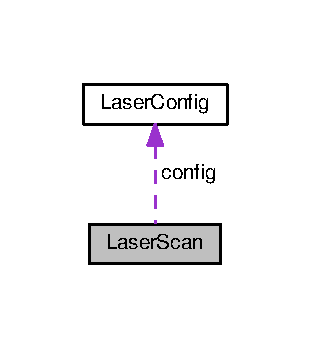
\includegraphics[width=149pt]{struct_laser_scan__coll__graph}
\end{center}
\end{figure}
\subsection*{Public Attributes}
\begin{DoxyCompactItemize}
\item 
std\+::vector$<$ float $>$ \hyperlink{struct_laser_scan_a4d059cb77f0f9f6e558db50c9993f7df}{ranges}\hypertarget{struct_laser_scan_a4d059cb77f0f9f6e558db50c9993f7df}{}\label{struct_laser_scan_a4d059cb77f0f9f6e558db50c9993f7df}

\begin{DoxyCompactList}\small\item\em Array of ranges. \end{DoxyCompactList}\item 
std\+::vector$<$ float $>$ \hyperlink{struct_laser_scan_a6e68040137d787ef7ef47580d147c503}{intensities}\hypertarget{struct_laser_scan_a6e68040137d787ef7ef47580d147c503}{}\label{struct_laser_scan_a6e68040137d787ef7ef47580d147c503}

\begin{DoxyCompactList}\small\item\em Array of intensities. \end{DoxyCompactList}\item 
uint64\+\_\+t \hyperlink{struct_laser_scan_ad37e2a54c7eff58cad7576d51916b859}{self\+\_\+time\+\_\+stamp}\hypertarget{struct_laser_scan_ad37e2a54c7eff58cad7576d51916b859}{}\label{struct_laser_scan_ad37e2a54c7eff58cad7576d51916b859}

\begin{DoxyCompactList}\small\item\em Self reported time stamp in nanoseconds. \end{DoxyCompactList}\item 
uint64\+\_\+t \hyperlink{struct_laser_scan_a1bb6b997ce698fbc516bc20ab3ba3399}{system\+\_\+time\+\_\+stamp}\hypertarget{struct_laser_scan_a1bb6b997ce698fbc516bc20ab3ba3399}{}\label{struct_laser_scan_a1bb6b997ce698fbc516bc20ab3ba3399}

\begin{DoxyCompactList}\small\item\em System time when first range was measured in nanoseconds. \end{DoxyCompactList}\item 
\hyperlink{struct_laser_config}{Laser\+Config} \hyperlink{struct_laser_scan_a5c7dd0b85432e62cf319f2ad4ec058b4}{config}\hypertarget{struct_laser_scan_a5c7dd0b85432e62cf319f2ad4ec058b4}{}\label{struct_laser_scan_a5c7dd0b85432e62cf319f2ad4ec058b4}

\begin{DoxyCompactList}\small\item\em Configuration of scan. \end{DoxyCompactList}\end{DoxyCompactItemize}


\subsection{Detailed Description}
A struct for returning laser readings from the Y\+D\+L\+I\+D\+AR current\+Angle = min\+\_\+angle + ang\+\_\+increment$\ast$index for( int i =0; i $<$ ranges.\+size(); i++) \{ double current\+Angle = config.\+min\+\_\+angle + i$\ast$config.ang\+\_\+increment; double current\+Distance = ranges\mbox{[}i\mbox{]}; \} 

The documentation for this struct was generated from the following file\+:\begin{DoxyCompactItemize}
\item 
include/ydlidar\+\_\+driver.\+h\end{DoxyCompactItemize}

\hypertarget{structlidar__ans__header}{}\section{lidar\+\_\+ans\+\_\+header Struct Reference}
\label{structlidar__ans__header}\index{lidar\+\_\+ans\+\_\+header@{lidar\+\_\+ans\+\_\+header}}
\subsection*{Public Attributes}
\begin{DoxyCompactItemize}
\item 
uint8\+\_\+t {\bfseries sync\+Byte1}\hypertarget{structlidar__ans__header_aeaa5beb7182c922d6d68697ecf60318a}{}\label{structlidar__ans__header_aeaa5beb7182c922d6d68697ecf60318a}

\item 
uint8\+\_\+t {\bfseries sync\+Byte2}\hypertarget{structlidar__ans__header_a9ce80818478513e1cb36de5a17917958}{}\label{structlidar__ans__header_a9ce80818478513e1cb36de5a17917958}

\item 
uint32\+\_\+t {\bfseries size}\+:30\hypertarget{structlidar__ans__header_a6e01bc2ec02153e40f3402790b917af3}{}\label{structlidar__ans__header_a6e01bc2ec02153e40f3402790b917af3}

\item 
uint32\+\_\+t {\bfseries sub\+Type}\+:2\hypertarget{structlidar__ans__header_abd31cd42537cebe7958b95d3f4a07169}{}\label{structlidar__ans__header_abd31cd42537cebe7958b95d3f4a07169}

\item 
uint8\+\_\+t {\bfseries type}\hypertarget{structlidar__ans__header_aab38102a1a266b5bfb842b10bf2804b2}{}\label{structlidar__ans__header_aab38102a1a266b5bfb842b10bf2804b2}

\end{DoxyCompactItemize}


The documentation for this struct was generated from the following file\+:\begin{DoxyCompactItemize}
\item 
include/ydlidar\+\_\+driver.\+h\end{DoxyCompactItemize}

\hypertarget{class_locker}{}\section{Locker Class Reference}
\label{class_locker}\index{Locker@{Locker}}
\subsection*{Public Types}
\begin{DoxyCompactItemize}
\item 
enum {\bfseries L\+O\+C\+K\+\_\+\+S\+T\+A\+T\+US} \{ {\bfseries L\+O\+C\+K\+\_\+\+OK} = 0, 
{\bfseries L\+O\+C\+K\+\_\+\+T\+I\+M\+E\+O\+UT} = -\/1, 
{\bfseries L\+O\+C\+K\+\_\+\+F\+A\+I\+L\+ED} = -\/2
 \}\hypertarget{class_locker_a9041a321dd3a61e8f4001bff198c1fba}{}\label{class_locker_a9041a321dd3a61e8f4001bff198c1fba}

\end{DoxyCompactItemize}
\subsection*{Public Member Functions}
\begin{DoxyCompactItemize}
\item 
Locker\+::\+L\+O\+C\+K\+\_\+\+S\+T\+A\+T\+US {\bfseries lock} (unsigned long timeout=0x\+F\+F\+F\+F\+F\+F\+F\+F)\hypertarget{class_locker_aabec65f1478f070c51c320ea202e9823}{}\label{class_locker_aabec65f1478f070c51c320ea202e9823}

\item 
void {\bfseries unlock} ()\hypertarget{class_locker_aafb16768c3b3a911002622b886000882}{}\label{class_locker_aafb16768c3b3a911002622b886000882}

\item 
pthread\+\_\+mutex\+\_\+t $\ast$ {\bfseries get\+Lock\+Handle} ()\hypertarget{class_locker_aed8d8d8cd1b14246396c8739ea4396a2}{}\label{class_locker_aed8d8d8cd1b14246396c8739ea4396a2}

\end{DoxyCompactItemize}
\subsection*{Protected Member Functions}
\begin{DoxyCompactItemize}
\item 
void {\bfseries init} ()\hypertarget{class_locker_a5eb30006ff65236fae5f8e67d2fe007c}{}\label{class_locker_a5eb30006ff65236fae5f8e67d2fe007c}

\item 
void {\bfseries release} ()\hypertarget{class_locker_a4780a62c558c6460fc34fcd935847934}{}\label{class_locker_a4780a62c558c6460fc34fcd935847934}

\end{DoxyCompactItemize}
\subsection*{Protected Attributes}
\begin{DoxyCompactItemize}
\item 
pthread\+\_\+mutex\+\_\+t {\bfseries \+\_\+lock}\hypertarget{class_locker_ac54c95aad09ef586cf91999f662f5b09}{}\label{class_locker_ac54c95aad09ef586cf91999f662f5b09}

\end{DoxyCompactItemize}


The documentation for this class was generated from the following file\+:\begin{DoxyCompactItemize}
\item 
include/locker.\+h\end{DoxyCompactItemize}

\hypertarget{classserial_1_1_millisecond_timer}{}\section{serial\+:\+:Millisecond\+Timer Class Reference}
\label{classserial_1_1_millisecond_timer}\index{serial\+::\+Millisecond\+Timer@{serial\+::\+Millisecond\+Timer}}
\subsection*{Public Member Functions}
\begin{DoxyCompactItemize}
\item 
{\bfseries Millisecond\+Timer} (const uint32\+\_\+t millis)\hypertarget{classserial_1_1_millisecond_timer_ac0f79f50e2859270bb1cb556377aee40}{}\label{classserial_1_1_millisecond_timer_ac0f79f50e2859270bb1cb556377aee40}

\item 
int64\+\_\+t {\bfseries remaining} ()\hypertarget{classserial_1_1_millisecond_timer_acb4d4e685a06fc7a2c24c90ac0970e35}{}\label{classserial_1_1_millisecond_timer_acb4d4e685a06fc7a2c24c90ac0970e35}

\end{DoxyCompactItemize}


The documentation for this class was generated from the following files\+:\begin{DoxyCompactItemize}
\item 
src/impl/unix/unix\+\_\+serial.\+h\item 
src/impl/unix/unix\+\_\+serial.\+cpp\end{DoxyCompactItemize}

\hypertarget{structnode__info}{}\section{node\+\_\+info Struct Reference}
\label{structnode__info}\index{node\+\_\+info@{node\+\_\+info}}
\subsection*{Public Attributes}
\begin{DoxyCompactItemize}
\item 
uint8\+\_\+t {\bfseries sync\+\_\+quality}\hypertarget{structnode__info_a45f5ed4efbe416d43171d63c669f02da}{}\label{structnode__info_a45f5ed4efbe416d43171d63c669f02da}

\item 
uint16\+\_\+t \hyperlink{structnode__info_a73e1d282a573f3daa74332fe29b90a26}{angle\+\_\+q6\+\_\+checkbit}\hypertarget{structnode__info_a73e1d282a573f3daa74332fe29b90a26}{}\label{structnode__info_a73e1d282a573f3daa74332fe29b90a26}

\begin{DoxyCompactList}\small\item\em 信号质量 \end{DoxyCompactList}\item 
uint16\+\_\+t \hyperlink{structnode__info_a82eaf27a6196e803d3618c83b052f78c}{distance\+\_\+q2}\hypertarget{structnode__info_a82eaf27a6196e803d3618c83b052f78c}{}\label{structnode__info_a82eaf27a6196e803d3618c83b052f78c}

\begin{DoxyCompactList}\small\item\em 测距点角度 \end{DoxyCompactList}\item 
uint64\+\_\+t \hyperlink{structnode__info_a92f30331da1d7d95f9998dcd3886574c}{stamp}\hypertarget{structnode__info_a92f30331da1d7d95f9998dcd3886574c}{}\label{structnode__info_a92f30331da1d7d95f9998dcd3886574c}

\begin{DoxyCompactList}\small\item\em 当前测距点距离 \end{DoxyCompactList}\item 
uint8\+\_\+t \hyperlink{structnode__info_a718a8a2f94497d5edea2be4550f74348}{scan\+\_\+frequence}\hypertarget{structnode__info_a718a8a2f94497d5edea2be4550f74348}{}\label{structnode__info_a718a8a2f94497d5edea2be4550f74348}

\begin{DoxyCompactList}\small\item\em 时间戳 \end{DoxyCompactList}\end{DoxyCompactItemize}


The documentation for this struct was generated from the following file\+:\begin{DoxyCompactItemize}
\item 
include/ydlidar\+\_\+driver.\+h\end{DoxyCompactItemize}

\hypertarget{structnode__package}{}\section{node\+\_\+package Struct Reference}
\label{structnode__package}\index{node\+\_\+package@{node\+\_\+package}}


Collaboration diagram for node\+\_\+package\+:\nopagebreak
\begin{figure}[H]
\begin{center}
\leavevmode
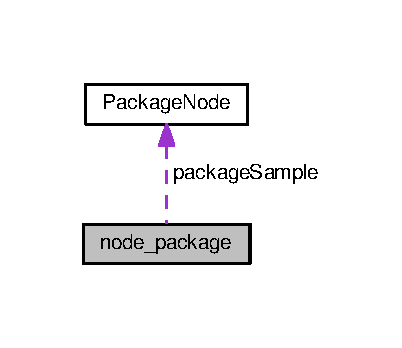
\includegraphics[width=193pt]{structnode__package__coll__graph}
\end{center}
\end{figure}
\subsection*{Public Attributes}
\begin{DoxyCompactItemize}
\item 
uint16\+\_\+t {\bfseries package\+\_\+\+Head}\hypertarget{structnode__package_a6d48d3a1d1ef718065a82e7495fa2b26}{}\label{structnode__package_a6d48d3a1d1ef718065a82e7495fa2b26}

\item 
uint8\+\_\+t {\bfseries package\+\_\+\+CT}\hypertarget{structnode__package_a3be7b81a7cc4b7ef7beb816ccd414579}{}\label{structnode__package_a3be7b81a7cc4b7ef7beb816ccd414579}

\item 
uint8\+\_\+t {\bfseries now\+Package\+Num}\hypertarget{structnode__package_aad0a75920ad5c1393f1b00904ece2d67}{}\label{structnode__package_aad0a75920ad5c1393f1b00904ece2d67}

\item 
uint16\+\_\+t {\bfseries package\+First\+Sample\+Angle}\hypertarget{structnode__package_ac224f6450e8bd5bd069149babc37e1c4}{}\label{structnode__package_ac224f6450e8bd5bd069149babc37e1c4}

\item 
uint16\+\_\+t {\bfseries package\+Last\+Sample\+Angle}\hypertarget{structnode__package_af5768e03270d3b7d7f58b3b82156dc2e}{}\label{structnode__package_af5768e03270d3b7d7f58b3b82156dc2e}

\item 
uint16\+\_\+t {\bfseries check\+Sum}\hypertarget{structnode__package_a4b6d9990da9343143161aae929bb986e}{}\label{structnode__package_a4b6d9990da9343143161aae929bb986e}

\item 
\hyperlink{struct_package_node}{Package\+Node} {\bfseries package\+Sample} \mbox{[}Package\+Sample\+Max\+Lngth\mbox{]}\hypertarget{structnode__package_a284fb0bbde964f2d43661ce6dcd8bca8}{}\label{structnode__package_a284fb0bbde964f2d43661ce6dcd8bca8}

\end{DoxyCompactItemize}


The documentation for this struct was generated from the following file\+:\begin{DoxyCompactItemize}
\item 
include/ydlidar\+\_\+driver.\+h\end{DoxyCompactItemize}

\hypertarget{structnode__packages}{}\section{node\+\_\+packages Struct Reference}
\label{structnode__packages}\index{node\+\_\+packages@{node\+\_\+packages}}
\subsection*{Public Attributes}
\begin{DoxyCompactItemize}
\item 
uint16\+\_\+t {\bfseries package\+\_\+\+Head}\hypertarget{structnode__packages_a1ed3121fde426c16fe5b5e8fac3c5431}{}\label{structnode__packages_a1ed3121fde426c16fe5b5e8fac3c5431}

\item 
uint8\+\_\+t {\bfseries package\+\_\+\+CT}\hypertarget{structnode__packages_a3365c5aeb9c44c7e7645fd056669437b}{}\label{structnode__packages_a3365c5aeb9c44c7e7645fd056669437b}

\item 
uint8\+\_\+t {\bfseries now\+Package\+Num}\hypertarget{structnode__packages_a7fc929fc56aa18d2229343e1c4079477}{}\label{structnode__packages_a7fc929fc56aa18d2229343e1c4079477}

\item 
uint16\+\_\+t {\bfseries package\+First\+Sample\+Angle}\hypertarget{structnode__packages_a48780f8343011c26cfa69bc0bcfb98d0}{}\label{structnode__packages_a48780f8343011c26cfa69bc0bcfb98d0}

\item 
uint16\+\_\+t {\bfseries package\+Last\+Sample\+Angle}\hypertarget{structnode__packages_a767062914a931ffc4ffc62292bdca610}{}\label{structnode__packages_a767062914a931ffc4ffc62292bdca610}

\item 
uint16\+\_\+t {\bfseries check\+Sum}\hypertarget{structnode__packages_a8ccc72e7cab7a3d4765ab5cc20097d41}{}\label{structnode__packages_a8ccc72e7cab7a3d4765ab5cc20097d41}

\item 
uint16\+\_\+t {\bfseries package\+Sample\+Distance} \mbox{[}Package\+Sample\+Max\+Lngth\mbox{]}\hypertarget{structnode__packages_a82b44c4cd7adf4f3c7923112b5438b0f}{}\label{structnode__packages_a82b44c4cd7adf4f3c7923112b5438b0f}

\end{DoxyCompactItemize}


The documentation for this struct was generated from the following file\+:\begin{DoxyCompactItemize}
\item 
include/ydlidar\+\_\+driver.\+h\end{DoxyCompactItemize}

\hypertarget{struct_package_node}{}\section{Package\+Node Struct Reference}
\label{struct_package_node}\index{Package\+Node@{Package\+Node}}
\subsection*{Public Attributes}
\begin{DoxyCompactItemize}
\item 
uint8\+\_\+t {\bfseries Pakage\+Sample\+Quality}\hypertarget{struct_package_node_aa93fa6630d9886ae0e381e06a72884cf}{}\label{struct_package_node_aa93fa6630d9886ae0e381e06a72884cf}

\item 
uint16\+\_\+t {\bfseries Pakage\+Sample\+Distance}\hypertarget{struct_package_node_a1ce84783c40c6f026a1b2dad2347d7a7}{}\label{struct_package_node_a1ce84783c40c6f026a1b2dad2347d7a7}

\end{DoxyCompactItemize}


The documentation for this struct was generated from the following file\+:\begin{DoxyCompactItemize}
\item 
/home/yang/tmp/sdk/include/ydlidar\+\_\+driver.\+h\end{DoxyCompactItemize}

\hypertarget{structserial_1_1_port_info}{}\section{serial\+:\+:Port\+Info Struct Reference}
\label{structserial_1_1_port_info}\index{serial\+::\+Port\+Info@{serial\+::\+Port\+Info}}


{\ttfamily \#include $<$serial.\+h$>$}



Collaboration diagram for serial\+:\+:Port\+Info\+:\nopagebreak
\begin{figure}[H]
\begin{center}
\leavevmode
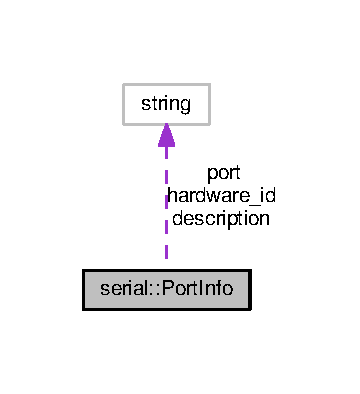
\includegraphics[width=173pt]{structserial_1_1_port_info__coll__graph}
\end{center}
\end{figure}
\subsection*{Public Attributes}
\begin{DoxyCompactItemize}
\item 
std\+::string \hyperlink{structserial_1_1_port_info_a5d4242cdd6c0d01260e24964af4c23d2}{port}
\item 
std\+::string \hyperlink{structserial_1_1_port_info_a2ba37dd33d47b554aef5c15c1fe8b872}{description}
\item 
std\+::string \hyperlink{structserial_1_1_port_info_a7d55368e1a4e6ccc9da6f4d339524837}{hardware\+\_\+id}
\end{DoxyCompactItemize}


\subsection{Detailed Description}
Structure that describes a serial device. 

\subsection{Member Data Documentation}
\index{serial\+::\+Port\+Info@{serial\+::\+Port\+Info}!description@{description}}
\index{description@{description}!serial\+::\+Port\+Info@{serial\+::\+Port\+Info}}
\subsubsection[{\texorpdfstring{description}{description}}]{\setlength{\rightskip}{0pt plus 5cm}std\+::string serial\+::\+Port\+Info\+::description}\hypertarget{structserial_1_1_port_info_a2ba37dd33d47b554aef5c15c1fe8b872}{}\label{structserial_1_1_port_info_a2ba37dd33d47b554aef5c15c1fe8b872}
Human readable description of serial device if available. \index{serial\+::\+Port\+Info@{serial\+::\+Port\+Info}!hardware\+\_\+id@{hardware\+\_\+id}}
\index{hardware\+\_\+id@{hardware\+\_\+id}!serial\+::\+Port\+Info@{serial\+::\+Port\+Info}}
\subsubsection[{\texorpdfstring{hardware\+\_\+id}{hardware_id}}]{\setlength{\rightskip}{0pt plus 5cm}std\+::string serial\+::\+Port\+Info\+::hardware\+\_\+id}\hypertarget{structserial_1_1_port_info_a7d55368e1a4e6ccc9da6f4d339524837}{}\label{structserial_1_1_port_info_a7d55368e1a4e6ccc9da6f4d339524837}
Hardware ID (e.\+g. V\+ID\+:P\+ID of U\+SB serial devices) or \char`\"{}n/a\char`\"{} if not available. \index{serial\+::\+Port\+Info@{serial\+::\+Port\+Info}!port@{port}}
\index{port@{port}!serial\+::\+Port\+Info@{serial\+::\+Port\+Info}}
\subsubsection[{\texorpdfstring{port}{port}}]{\setlength{\rightskip}{0pt plus 5cm}std\+::string serial\+::\+Port\+Info\+::port}\hypertarget{structserial_1_1_port_info_a5d4242cdd6c0d01260e24964af4c23d2}{}\label{structserial_1_1_port_info_a5d4242cdd6c0d01260e24964af4c23d2}
Address of the serial port (this can be passed to the constructor of \hyperlink{classserial_1_1_serial}{Serial}). 

The documentation for this struct was generated from the following file\+:\begin{DoxyCompactItemize}
\item 
/home/yang/tmp/sdk/include/serial.\+h\end{DoxyCompactItemize}

\hypertarget{structsampling__rate}{}\section{sampling\+\_\+rate Struct Reference}
\label{structsampling__rate}\index{sampling\+\_\+rate@{sampling\+\_\+rate}}
\subsection*{Public Attributes}
\begin{DoxyCompactItemize}
\item 
uint8\+\_\+t \hyperlink{structsampling__rate_a8d860fbedd930d2022fe7bb6cf1f78b6}{rate}\hypertarget{structsampling__rate_a8d860fbedd930d2022fe7bb6cf1f78b6}{}\label{structsampling__rate_a8d860fbedd930d2022fe7bb6cf1f78b6}

\begin{DoxyCompactList}\small\item\em 采样频率 \end{DoxyCompactList}\end{DoxyCompactItemize}


The documentation for this struct was generated from the following file\+:\begin{DoxyCompactItemize}
\item 
include/ydlidar\+\_\+driver.\+h\end{DoxyCompactItemize}

\hypertarget{structscan__exposure}{}\section{scan\+\_\+exposure Struct Reference}
\label{structscan__exposure}\index{scan\+\_\+exposure@{scan\+\_\+exposure}}
\subsection*{Public Attributes}
\begin{DoxyCompactItemize}
\item 
uint8\+\_\+t \hyperlink{structscan__exposure_a49591ef660667fcd1c3e1c2f3d764004}{exposure}\hypertarget{structscan__exposure_a49591ef660667fcd1c3e1c2f3d764004}{}\label{structscan__exposure_a49591ef660667fcd1c3e1c2f3d764004}

\begin{DoxyCompactList}\small\item\em 低光功率模式 \end{DoxyCompactList}\end{DoxyCompactItemize}


The documentation for this struct was generated from the following file\+:\begin{DoxyCompactItemize}
\item 
include/ydlidar\+\_\+driver.\+h\end{DoxyCompactItemize}

\hypertarget{structscan__frequency}{}\section{scan\+\_\+frequency Struct Reference}
\label{structscan__frequency}\index{scan\+\_\+frequency@{scan\+\_\+frequency}}
\subsection*{Public Attributes}
\begin{DoxyCompactItemize}
\item 
uint32\+\_\+t \hyperlink{structscan__frequency_ae4f2152e77416cff02f44452355f2808}{frequency}
\end{DoxyCompactItemize}


\subsection{Member Data Documentation}
\index{scan\+\_\+frequency@{scan\+\_\+frequency}!frequency@{frequency}}
\index{frequency@{frequency}!scan\+\_\+frequency@{scan\+\_\+frequency}}
\subsubsection[{\texorpdfstring{frequency}{frequency}}]{\setlength{\rightskip}{0pt plus 5cm}uint32\+\_\+t scan\+\_\+frequency\+::frequency}\hypertarget{structscan__frequency_ae4f2152e77416cff02f44452355f2808}{}\label{structscan__frequency_ae4f2152e77416cff02f44452355f2808}
扫描频率. 

The documentation for this struct was generated from the following file\+:\begin{DoxyCompactItemize}
\item 
/home/yang/tmp/sdk/include/ydlidar\+\_\+driver.\+h\end{DoxyCompactItemize}

\hypertarget{structscan__heart__beat}{}\section{scan\+\_\+heart\+\_\+beat Struct Reference}
\label{structscan__heart__beat}\index{scan\+\_\+heart\+\_\+beat@{scan\+\_\+heart\+\_\+beat}}
\subsection*{Public Attributes}
\begin{DoxyCompactItemize}
\item 
uint8\+\_\+t \hyperlink{structscan__heart__beat_a2b75f0058448601c590dda44d962d5c9}{enable}\hypertarget{structscan__heart__beat_a2b75f0058448601c590dda44d962d5c9}{}\label{structscan__heart__beat_a2b75f0058448601c590dda44d962d5c9}

\begin{DoxyCompactList}\small\item\em 掉电保护状态 \end{DoxyCompactList}\end{DoxyCompactItemize}


The documentation for this struct was generated from the following file\+:\begin{DoxyCompactItemize}
\item 
include/ydlidar\+\_\+driver.\+h\end{DoxyCompactItemize}

\hypertarget{structscan__points}{}\section{scan\+\_\+points Struct Reference}
\label{structscan__points}\index{scan\+\_\+points@{scan\+\_\+points}}
\subsection*{Public Attributes}
\begin{DoxyCompactItemize}
\item 
uint8\+\_\+t {\bfseries flag}\hypertarget{structscan__points_ae2f1ac4c7f2d11a3db2eec0da4eae66e}{}\label{structscan__points_ae2f1ac4c7f2d11a3db2eec0da4eae66e}

\end{DoxyCompactItemize}


The documentation for this struct was generated from the following file\+:\begin{DoxyCompactItemize}
\item 
include/ydlidar\+\_\+driver.\+h\end{DoxyCompactItemize}

\hypertarget{structscan__rotation}{}\section{scan\+\_\+rotation Struct Reference}
\label{structscan__rotation}\index{scan\+\_\+rotation@{scan\+\_\+rotation}}
\subsection*{Public Attributes}
\begin{DoxyCompactItemize}
\item 
uint8\+\_\+t {\bfseries rotation}\hypertarget{structscan__rotation_a22cb3689e04952bbd07cdac97ecad4a0}{}\label{structscan__rotation_a22cb3689e04952bbd07cdac97ecad4a0}

\end{DoxyCompactItemize}


The documentation for this struct was generated from the following file\+:\begin{DoxyCompactItemize}
\item 
/home/yang/tmp/sdk/include/ydlidar\+\_\+driver.\+h\end{DoxyCompactItemize}

\hypertarget{structscan_dot}{}\section{scan\+Dot Struct Reference}
\label{structscan_dot}\index{scan\+Dot@{scan\+Dot}}
\subsection*{Public Attributes}
\begin{DoxyCompactItemize}
\item 
uint8\+\_\+t {\bfseries quality}\hypertarget{structscan_dot_ad4bb237b2544b87dd6d57a49b1168bc1}{}\label{structscan_dot_ad4bb237b2544b87dd6d57a49b1168bc1}

\item 
float {\bfseries angle}\hypertarget{structscan_dot_a97b573cb811b6ca7318c485a0c67e250}{}\label{structscan_dot_a97b573cb811b6ca7318c485a0c67e250}

\item 
float {\bfseries dist}\hypertarget{structscan_dot_af52fcb416f886a7f505c8baf6cabc87f}{}\label{structscan_dot_af52fcb416f886a7f505c8baf6cabc87f}

\end{DoxyCompactItemize}


The documentation for this struct was generated from the following file\+:\begin{DoxyCompactItemize}
\item 
include/ydlidar\+\_\+driver.\+h\end{DoxyCompactItemize}

\hypertarget{class_scoped_locker}{}\section{Scoped\+Locker Class Reference}
\label{class_scoped_locker}\index{Scoped\+Locker@{Scoped\+Locker}}


Collaboration diagram for Scoped\+Locker\+:\nopagebreak
\begin{figure}[H]
\begin{center}
\leavevmode
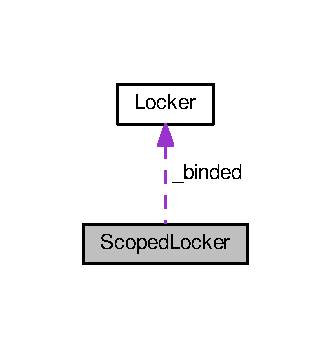
\includegraphics[width=159pt]{class_scoped_locker__coll__graph}
\end{center}
\end{figure}
\subsection*{Public Member Functions}
\begin{DoxyCompactItemize}
\item 
{\bfseries Scoped\+Locker} (\hyperlink{class_locker}{Locker} \&l)\hypertarget{class_scoped_locker_a934b25a7af086a7230e96256ab2f54be}{}\label{class_scoped_locker_a934b25a7af086a7230e96256ab2f54be}

\item 
void {\bfseries force\+Unlock} ()\hypertarget{class_scoped_locker_a5a9c0873fb7c11ea588b627497208a41}{}\label{class_scoped_locker_a5a9c0873fb7c11ea588b627497208a41}

\end{DoxyCompactItemize}
\subsection*{Public Attributes}
\begin{DoxyCompactItemize}
\item 
\hyperlink{class_locker}{Locker} \& {\bfseries \+\_\+binded}\hypertarget{class_scoped_locker_abfc68c3a65391f09b81de01492bc60be}{}\label{class_scoped_locker_abfc68c3a65391f09b81de01492bc60be}

\end{DoxyCompactItemize}


The documentation for this class was generated from the following file\+:\begin{DoxyCompactItemize}
\item 
include/locker.\+h\end{DoxyCompactItemize}

\hypertarget{classserial_1_1_serial_1_1_scoped_read_lock}{}\section{serial\+:\+:Serial\+:\+:Scoped\+Read\+Lock Class Reference}
\label{classserial_1_1_serial_1_1_scoped_read_lock}\index{serial\+::\+Serial\+::\+Scoped\+Read\+Lock@{serial\+::\+Serial\+::\+Scoped\+Read\+Lock}}
\subsection*{Public Member Functions}
\begin{DoxyCompactItemize}
\item 
{\bfseries Scoped\+Read\+Lock} (\hyperlink{classserial_1_1serial_1_1_serial_1_1_serial_impl}{Serial\+Impl} $\ast$pimpl)\hypertarget{classserial_1_1_serial_1_1_scoped_read_lock_a54f59663807d8adfe6db712ee6103503}{}\label{classserial_1_1_serial_1_1_scoped_read_lock_a54f59663807d8adfe6db712ee6103503}

\end{DoxyCompactItemize}


The documentation for this class was generated from the following file\+:\begin{DoxyCompactItemize}
\item 
src/serial.\+cpp\end{DoxyCompactItemize}

\hypertarget{classserial_1_1_serial_1_1_scoped_write_lock}{}\section{serial\+:\+:Serial\+:\+:Scoped\+Write\+Lock Class Reference}
\label{classserial_1_1_serial_1_1_scoped_write_lock}\index{serial\+::\+Serial\+::\+Scoped\+Write\+Lock@{serial\+::\+Serial\+::\+Scoped\+Write\+Lock}}
\subsection*{Public Member Functions}
\begin{DoxyCompactItemize}
\item 
{\bfseries Scoped\+Write\+Lock} (\hyperlink{classserial_1_1serial_1_1_serial_1_1_serial_impl}{Serial\+Impl} $\ast$pimpl)\hypertarget{classserial_1_1_serial_1_1_scoped_write_lock_a662173968431aee3d6f204c354b20225}{}\label{classserial_1_1_serial_1_1_scoped_write_lock_a662173968431aee3d6f204c354b20225}

\end{DoxyCompactItemize}


The documentation for this class was generated from the following file\+:\begin{DoxyCompactItemize}
\item 
/home/yang/tmp/sdk/src/serial.\+cpp\end{DoxyCompactItemize}

\hypertarget{classserial_1_1_serial}{}\section{serial\+:\+:Serial Class Reference}
\label{classserial_1_1_serial}\index{serial\+::\+Serial@{serial\+::\+Serial}}


{\ttfamily \#include $<$serial.\+h$>$}

\subsection*{Classes}
\begin{DoxyCompactItemize}
\item 
class \hyperlink{classserial_1_1_serial_1_1_scoped_read_lock}{Scoped\+Read\+Lock}
\item 
class \hyperlink{classserial_1_1_serial_1_1_scoped_write_lock}{Scoped\+Write\+Lock}
\item 
class \hyperlink{classserial_1_1serial_1_1_serial_1_1_serial_impl}{Serial\+Impl}
\end{DoxyCompactItemize}
\subsection*{Public Member Functions}
\begin{DoxyCompactItemize}
\item 
\hyperlink{classserial_1_1_serial_aecbc4cc1723143805ae5a4aa79ba9332}{Serial} (const std\+::string \&port=\char`\"{}\char`\"{}, uint32\+\_\+t baudrate=9600, \hyperlink{structserial_1_1_timeout}{Timeout} timeout=\hyperlink{structserial_1_1_timeout}{Timeout}(), \hyperlink{namespaceserial_a00b3281fa11cea770c0b0c8a106080f8}{bytesize\+\_\+t} bytesize=eightbits, \hyperlink{namespaceserial_a8f45d26bf7c9a06659e75b5004a50481}{parity\+\_\+t} parity=parity\+\_\+none, \hyperlink{namespaceserial_af5b116611d6628a3aa8f788fdc09f469}{stopbits\+\_\+t} stopbits=stopbits\+\_\+one, \hyperlink{namespaceserial_a93ef57a314b4e562f9eded6c15d34351}{flowcontrol\+\_\+t} flowcontrol=flowcontrol\+\_\+none)
\item 
virtual \hyperlink{classserial_1_1_serial_a071000a2f5f77a40df8311fad5044481}{$\sim$\+Serial} ()
\item 
bool \hyperlink{classserial_1_1_serial_aa4403ddb51e9d209fd86ed316f0ee9b4}{open} ()
\item 
bool \hyperlink{classserial_1_1_serial_a48458f741d0fdcc5623b4daa079cbf78}{is\+Open} () const 
\item 
void \hyperlink{classserial_1_1_serial_a501082725b61e4baf615266065bbac5f}{close} ()
\item 
size\+\_\+t \hyperlink{classserial_1_1_serial_ab5fae6cebb8e34345ca1f55cbccc4698}{available} ()
\item 
bool \hyperlink{classserial_1_1_serial_a59bd8d40309769e8eed91dd3684e0000}{wait\+Readable} ()
\item 
void \hyperlink{classserial_1_1_serial_a35c0f6ff20c142a5210dde288731f954}{wait\+Byte\+Times} (size\+\_\+t count)
\item 
int {\bfseries waitfordata} (size\+\_\+t data\+\_\+count, uint32\+\_\+t timeout, size\+\_\+t $\ast$returned\+\_\+size)\hypertarget{classserial_1_1_serial_aa94e4ca3b2b803e3145c99fe063ae09b}{}\label{classserial_1_1_serial_aa94e4ca3b2b803e3145c99fe063ae09b}

\item 
size\+\_\+t \hyperlink{classserial_1_1_serial_a01fc2e3d77cb7d70069de87eca1400e9}{read} (uint8\+\_\+t $\ast$buffer, size\+\_\+t size)
\item 
size\+\_\+t \hyperlink{classserial_1_1_serial_a3ecd4645c76548ba079eab6f2f46adfb}{read} (std\+::vector$<$ uint8\+\_\+t $>$ \&buffer, size\+\_\+t size=1)
\item 
size\+\_\+t \hyperlink{classserial_1_1_serial_ad6c6637fdf8edd85c3a6a63d98fc18f7}{read} (std\+::string \&buffer, size\+\_\+t size=1)
\item 
std\+::string \hyperlink{classserial_1_1_serial_aa52fbf7d23fb761a46e2400829d2b77a}{read} (size\+\_\+t size=1)
\item 
size\+\_\+t \hyperlink{classserial_1_1_serial_a010b18ec545dfe1a7bb1c95be4bdaa54}{readline} (std\+::string \&buffer, size\+\_\+t size=65536, std\+::string eol=\char`\"{}\textbackslash{}n\char`\"{})
\item 
std\+::string \hyperlink{classserial_1_1_serial_a04177f637cc02f92ec0492d377528b2a}{readline} (size\+\_\+t size=65536, std\+::string eol=\char`\"{}\textbackslash{}n\char`\"{})
\item 
std\+::vector$<$ std\+::string $>$ \hyperlink{classserial_1_1_serial_a2ff222081c30ee4343498c6cc5c14b10}{readlines} (size\+\_\+t size=65536, std\+::string eol=\char`\"{}\textbackslash{}n\char`\"{})
\item 
size\+\_\+t \hyperlink{classserial_1_1_serial_a3275e8456850998c0ac46b2768ab9258}{write} (const uint8\+\_\+t $\ast$data, size\+\_\+t size)
\item 
size\+\_\+t \hyperlink{classserial_1_1_serial_a9c2827088d82ee82f245ffa106fa7d10}{write} (const std\+::vector$<$ uint8\+\_\+t $>$ \&data)
\item 
size\+\_\+t \hyperlink{classserial_1_1_serial_a7c92c0307b86a935f6623953eec66460}{write} (const std\+::string \&data)
\item 
void \hyperlink{classserial_1_1_serial_a127104a1b211c46e4cad9002123e6ea8}{set\+Port} (const std\+::string \&port)
\item 
std\+::string \hyperlink{classserial_1_1_serial_a56eafe1694c92655d79993ce7139f0bf}{get\+Port} () const 
\item 
void \hyperlink{classserial_1_1_serial_a5b1a4e05b1690d29ba1ae14a9079434c}{set\+Timeout} (\hyperlink{structserial_1_1_timeout}{Timeout} \&timeout)
\item 
void \hyperlink{classserial_1_1_serial_a4b4be39af3e1c68bc6ac09cb55788c86}{set\+Timeout} (uint32\+\_\+t inter\+\_\+byte\+\_\+timeout, uint32\+\_\+t read\+\_\+timeout\+\_\+constant, uint32\+\_\+t read\+\_\+timeout\+\_\+multiplier, uint32\+\_\+t write\+\_\+timeout\+\_\+constant, uint32\+\_\+t write\+\_\+timeout\+\_\+multiplier)
\item 
\hyperlink{structserial_1_1_timeout}{Timeout} \hyperlink{classserial_1_1_serial_a13023f118c75b27fa2f0280d2d1c2a20}{get\+Timeout} () const 
\item 
bool \hyperlink{classserial_1_1_serial_a05085fc22adee665698bdfd9b7b9783f}{set\+Baudrate} (uint32\+\_\+t baudrate)
\item 
uint32\+\_\+t \hyperlink{classserial_1_1_serial_a7a6ca1f8d8e68742e95b7f8dc8e9a1fa}{get\+Baudrate} () const 
\item 
bool \hyperlink{classserial_1_1_serial_a8adf3dcd68fb1b85ce30c8b443e5868a}{set\+Bytesize} (\hyperlink{namespaceserial_a00b3281fa11cea770c0b0c8a106080f8}{bytesize\+\_\+t} bytesize)
\item 
\hyperlink{namespaceserial_a00b3281fa11cea770c0b0c8a106080f8}{bytesize\+\_\+t} \hyperlink{classserial_1_1_serial_ac735ef88a54659e2d0b3ae674c5f0a41}{get\+Bytesize} () const 
\item 
bool \hyperlink{classserial_1_1_serial_af471db5d3a89128430e7e3c5389cd08a}{set\+Parity} (\hyperlink{namespaceserial_a8f45d26bf7c9a06659e75b5004a50481}{parity\+\_\+t} parity)
\item 
\hyperlink{namespaceserial_a8f45d26bf7c9a06659e75b5004a50481}{parity\+\_\+t} \hyperlink{classserial_1_1_serial_a80e5d87b1e93b4c5a9d6f2cc7110b3c4}{get\+Parity} () const 
\item 
bool \hyperlink{classserial_1_1_serial_a0c690a31516cd11c521ba3aff4bafc4e}{set\+Stopbits} (\hyperlink{namespaceserial_af5b116611d6628a3aa8f788fdc09f469}{stopbits\+\_\+t} stopbits)
\item 
\hyperlink{namespaceserial_af5b116611d6628a3aa8f788fdc09f469}{stopbits\+\_\+t} \hyperlink{classserial_1_1_serial_a81ee96ec2fdb80d1851430d9e2c4698b}{get\+Stopbits} () const 
\item 
bool \hyperlink{classserial_1_1_serial_a76e56ce22e2706b8954a1dc9c5188c92}{set\+Flowcontrol} (\hyperlink{namespaceserial_a93ef57a314b4e562f9eded6c15d34351}{flowcontrol\+\_\+t} flowcontrol)
\item 
\hyperlink{namespaceserial_a93ef57a314b4e562f9eded6c15d34351}{flowcontrol\+\_\+t} \hyperlink{classserial_1_1_serial_ad793526755625a59a0bf9d4cc0ea1755}{get\+Flowcontrol} () const 
\item 
void \hyperlink{classserial_1_1_serial_a45a7676a6e6c775cd549e889e714b5bb}{flush} ()
\item 
void \hyperlink{classserial_1_1_serial_aa7432cbada95a7eac6d71a107cf2eaa3}{flush\+Input} ()
\item 
void \hyperlink{classserial_1_1_serial_a95e0d6dcf2b7b9aa45225bfb1647c427}{flush\+Output} ()
\item 
void \hyperlink{classserial_1_1_serial_ab35e474beb136258cbeb04978be27455}{send\+Break} (int duration)
\item 
bool \hyperlink{classserial_1_1_serial_abb7eef9db06c582e2e504733b4150968}{set\+Break} (bool level=true)
\item 
bool \hyperlink{classserial_1_1_serial_a7c91f22768107389f52d80d691994fc7}{set\+R\+TS} (bool level=true)
\item 
bool \hyperlink{classserial_1_1_serial_a4c8a44a1e6ce42f8cb521d9a4e10bc59}{set\+D\+TR} (bool level=true)
\item 
bool \hyperlink{classserial_1_1_serial_a9d889dc0ec2cec50a620650f10cf8e83}{wait\+For\+Change} ()
\item 
bool \hyperlink{classserial_1_1_serial_a97603438c9ded81a886f914b7a335d7f}{get\+C\+TS} ()
\item 
bool \hyperlink{classserial_1_1_serial_a91a00816bce6a163ea022b4cf8d4ce0e}{get\+D\+SR} ()
\item 
bool \hyperlink{classserial_1_1_serial_a29a1f68b9a238e9a6a833373855708ce}{get\+RI} ()
\item 
bool \hyperlink{classserial_1_1_serial_a5a7c1a8e363b530147970155d0f6fe8d}{get\+CD} ()
\item 
uint32\+\_\+t \hyperlink{classserial_1_1_serial_a8b7ad05b2521db6bbf184108f59e105e}{get\+Byte\+Time} ()
\end{DoxyCompactItemize}


\subsection{Detailed Description}
Class that provides a portable serial port interface. 

\subsection{Constructor \& Destructor Documentation}
\index{serial\+::\+Serial@{serial\+::\+Serial}!Serial@{Serial}}
\index{Serial@{Serial}!serial\+::\+Serial@{serial\+::\+Serial}}
\subsubsection[{\texorpdfstring{Serial(const std\+::string \&port="""", uint32\+\_\+t baudrate=9600, Timeout timeout=\+Timeout(), bytesize\+\_\+t bytesize=eightbits, parity\+\_\+t parity=parity\+\_\+none, stopbits\+\_\+t stopbits=stopbits\+\_\+one, flowcontrol\+\_\+t flowcontrol=flowcontrol\+\_\+none)}{Serial(const std::string &port="", uint32_t baudrate=9600, Timeout timeout=Timeout(), bytesize_t bytesize=eightbits, parity_t parity=parity_none, stopbits_t stopbits=stopbits_one, flowcontrol_t flowcontrol=flowcontrol_none)}}]{\setlength{\rightskip}{0pt plus 5cm}serial\+::\+Serial\+::\+Serial (
\begin{DoxyParamCaption}
\item[{const std\+::string \&}]{port = {\ttfamily \char`\"{}\char`\"{}}, }
\item[{uint32\+\_\+t}]{baudrate = {\ttfamily 9600}, }
\item[{{\bf Timeout}}]{timeout = {\ttfamily {\bf Timeout}()}, }
\item[{{\bf bytesize\+\_\+t}}]{bytesize = {\ttfamily eightbits}, }
\item[{{\bf parity\+\_\+t}}]{parity = {\ttfamily parity\+\_\+none}, }
\item[{{\bf stopbits\+\_\+t}}]{stopbits = {\ttfamily stopbits\+\_\+one}, }
\item[{{\bf flowcontrol\+\_\+t}}]{flowcontrol = {\ttfamily flowcontrol\+\_\+none}}
\end{DoxyParamCaption}
)\hspace{0.3cm}{\ttfamily [explicit]}}\hypertarget{classserial_1_1_serial_aecbc4cc1723143805ae5a4aa79ba9332}{}\label{classserial_1_1_serial_aecbc4cc1723143805ae5a4aa79ba9332}
Creates a \hyperlink{classserial_1_1_serial}{Serial} object and opens the port if a port is specified, otherwise it remains closed until \hyperlink{classserial_1_1_serial_aa4403ddb51e9d209fd86ed316f0ee9b4}{serial\+::\+Serial\+::open} is called.


\begin{DoxyParams}{Parameters}
{\em port} & A std\+::string containing the address of the serial port, which would be something like \textquotesingle{}C\+O\+M1\textquotesingle{} on Windows and \textquotesingle{}/dev/tty\+S0\textquotesingle{} on Linux.\\
\hline
{\em baudrate} & An unsigned 32-\/bit integer that represents the baudrate\\
\hline
{\em timeout} & A \hyperlink{structserial_1_1_timeout}{serial\+::\+Timeout} struct that defines the timeout conditions for the serial port. \\
\hline
\end{DoxyParams}
\begin{DoxySeeAlso}{See also}
\hyperlink{structserial_1_1_timeout}{serial\+::\+Timeout}
\end{DoxySeeAlso}

\begin{DoxyParams}{Parameters}
{\em bytesize} & Size of each byte in the serial transmission of data, default is eightbits, possible values are\+: fivebits, sixbits, sevenbits, eightbits\\
\hline
{\em parity} & Method of parity, default is parity\+\_\+none, possible values are\+: parity\+\_\+none, parity\+\_\+odd, parity\+\_\+even\\
\hline
{\em stopbits} & Number of stop bits used, default is stopbits\+\_\+one, possible values are\+: stopbits\+\_\+one, stopbits\+\_\+one\+\_\+point\+\_\+five, stopbits\+\_\+two\\
\hline
{\em flowcontrol} & Type of flowcontrol used, default is flowcontrol\+\_\+none, possible values are\+: flowcontrol\+\_\+none, flowcontrol\+\_\+software, flowcontrol\+\_\+hardware\\
\hline
\end{DoxyParams}

\begin{DoxyExceptions}{Exceptions}
{\em serial\+::\+Port\+Not\+Opened\+Exception} & \\
\hline
{\em serial\+::\+I\+O\+Exception} & \\
\hline
{\em std\+::invalid\+\_\+argument} & \\
\hline
\end{DoxyExceptions}
\index{serial\+::\+Serial@{serial\+::\+Serial}!````~Serial@{$\sim$\+Serial}}
\index{````~Serial@{$\sim$\+Serial}!serial\+::\+Serial@{serial\+::\+Serial}}
\subsubsection[{\texorpdfstring{$\sim$\+Serial()}{~Serial()}}]{\setlength{\rightskip}{0pt plus 5cm}serial\+::\+Serial\+::$\sim$\+Serial (
\begin{DoxyParamCaption}
{}
\end{DoxyParamCaption}
)\hspace{0.3cm}{\ttfamily [virtual]}}\hypertarget{classserial_1_1_serial_a071000a2f5f77a40df8311fad5044481}{}\label{classserial_1_1_serial_a071000a2f5f77a40df8311fad5044481}
Destructor 

\subsection{Member Function Documentation}
\index{serial\+::\+Serial@{serial\+::\+Serial}!available@{available}}
\index{available@{available}!serial\+::\+Serial@{serial\+::\+Serial}}
\subsubsection[{\texorpdfstring{available()}{available()}}]{\setlength{\rightskip}{0pt plus 5cm}size\+\_\+t serial\+::\+Serial\+::available (
\begin{DoxyParamCaption}
{}
\end{DoxyParamCaption}
)}\hypertarget{classserial_1_1_serial_ab5fae6cebb8e34345ca1f55cbccc4698}{}\label{classserial_1_1_serial_ab5fae6cebb8e34345ca1f55cbccc4698}
Return the number of characters in the buffer. \index{serial\+::\+Serial@{serial\+::\+Serial}!close@{close}}
\index{close@{close}!serial\+::\+Serial@{serial\+::\+Serial}}
\subsubsection[{\texorpdfstring{close()}{close()}}]{\setlength{\rightskip}{0pt plus 5cm}void serial\+::\+Serial\+::close (
\begin{DoxyParamCaption}
{}
\end{DoxyParamCaption}
)}\hypertarget{classserial_1_1_serial_a501082725b61e4baf615266065bbac5f}{}\label{classserial_1_1_serial_a501082725b61e4baf615266065bbac5f}
Closes the serial port. \index{serial\+::\+Serial@{serial\+::\+Serial}!flush@{flush}}
\index{flush@{flush}!serial\+::\+Serial@{serial\+::\+Serial}}
\subsubsection[{\texorpdfstring{flush()}{flush()}}]{\setlength{\rightskip}{0pt plus 5cm}void serial\+::\+Serial\+::flush (
\begin{DoxyParamCaption}
{}
\end{DoxyParamCaption}
)}\hypertarget{classserial_1_1_serial_a45a7676a6e6c775cd549e889e714b5bb}{}\label{classserial_1_1_serial_a45a7676a6e6c775cd549e889e714b5bb}
Flush the input and output buffers \index{serial\+::\+Serial@{serial\+::\+Serial}!flush\+Input@{flush\+Input}}
\index{flush\+Input@{flush\+Input}!serial\+::\+Serial@{serial\+::\+Serial}}
\subsubsection[{\texorpdfstring{flush\+Input()}{flushInput()}}]{\setlength{\rightskip}{0pt plus 5cm}void serial\+::\+Serial\+::flush\+Input (
\begin{DoxyParamCaption}
{}
\end{DoxyParamCaption}
)}\hypertarget{classserial_1_1_serial_aa7432cbada95a7eac6d71a107cf2eaa3}{}\label{classserial_1_1_serial_aa7432cbada95a7eac6d71a107cf2eaa3}
Flush only the input buffer \index{serial\+::\+Serial@{serial\+::\+Serial}!flush\+Output@{flush\+Output}}
\index{flush\+Output@{flush\+Output}!serial\+::\+Serial@{serial\+::\+Serial}}
\subsubsection[{\texorpdfstring{flush\+Output()}{flushOutput()}}]{\setlength{\rightskip}{0pt plus 5cm}void serial\+::\+Serial\+::flush\+Output (
\begin{DoxyParamCaption}
{}
\end{DoxyParamCaption}
)}\hypertarget{classserial_1_1_serial_a95e0d6dcf2b7b9aa45225bfb1647c427}{}\label{classserial_1_1_serial_a95e0d6dcf2b7b9aa45225bfb1647c427}
Flush only the output buffer \index{serial\+::\+Serial@{serial\+::\+Serial}!get\+Baudrate@{get\+Baudrate}}
\index{get\+Baudrate@{get\+Baudrate}!serial\+::\+Serial@{serial\+::\+Serial}}
\subsubsection[{\texorpdfstring{get\+Baudrate() const }{getBaudrate() const }}]{\setlength{\rightskip}{0pt plus 5cm}uint32\+\_\+t serial\+::\+Serial\+::get\+Baudrate (
\begin{DoxyParamCaption}
{}
\end{DoxyParamCaption}
) const}\hypertarget{classserial_1_1_serial_a7a6ca1f8d8e68742e95b7f8dc8e9a1fa}{}\label{classserial_1_1_serial_a7a6ca1f8d8e68742e95b7f8dc8e9a1fa}
Gets the baudrate for the serial port.

\begin{DoxyReturn}{Returns}
An integer that sets the baud rate for the serial port.
\end{DoxyReturn}
\begin{DoxySeeAlso}{See also}
\hyperlink{classserial_1_1_serial_a05085fc22adee665698bdfd9b7b9783f}{Serial\+::set\+Baudrate}
\end{DoxySeeAlso}
\textbackslash{} \index{serial\+::\+Serial@{serial\+::\+Serial}!get\+Bytesize@{get\+Bytesize}}
\index{get\+Bytesize@{get\+Bytesize}!serial\+::\+Serial@{serial\+::\+Serial}}
\subsubsection[{\texorpdfstring{get\+Bytesize() const }{getBytesize() const }}]{\setlength{\rightskip}{0pt plus 5cm}{\bf bytesize\+\_\+t} serial\+::\+Serial\+::get\+Bytesize (
\begin{DoxyParamCaption}
{}
\end{DoxyParamCaption}
) const}\hypertarget{classserial_1_1_serial_ac735ef88a54659e2d0b3ae674c5f0a41}{}\label{classserial_1_1_serial_ac735ef88a54659e2d0b3ae674c5f0a41}
Gets the bytesize for the serial port.

\begin{DoxySeeAlso}{See also}
\hyperlink{classserial_1_1_serial_a8adf3dcd68fb1b85ce30c8b443e5868a}{Serial\+::set\+Bytesize}
\end{DoxySeeAlso}
\textbackslash{} \index{serial\+::\+Serial@{serial\+::\+Serial}!get\+Byte\+Time@{get\+Byte\+Time}}
\index{get\+Byte\+Time@{get\+Byte\+Time}!serial\+::\+Serial@{serial\+::\+Serial}}
\subsubsection[{\texorpdfstring{get\+Byte\+Time()}{getByteTime()}}]{\setlength{\rightskip}{0pt plus 5cm}uint32\+\_\+t serial\+::\+Serial\+::get\+Byte\+Time (
\begin{DoxyParamCaption}
{}
\end{DoxyParamCaption}
)}\hypertarget{classserial_1_1_serial_a8b7ad05b2521db6bbf184108f59e105e}{}\label{classserial_1_1_serial_a8b7ad05b2521db6bbf184108f59e105e}
Returns the singal byte time. \index{serial\+::\+Serial@{serial\+::\+Serial}!get\+CD@{get\+CD}}
\index{get\+CD@{get\+CD}!serial\+::\+Serial@{serial\+::\+Serial}}
\subsubsection[{\texorpdfstring{get\+C\+D()}{getCD()}}]{\setlength{\rightskip}{0pt plus 5cm}bool serial\+::\+Serial\+::get\+CD (
\begin{DoxyParamCaption}
{}
\end{DoxyParamCaption}
)}\hypertarget{classserial_1_1_serial_a5a7c1a8e363b530147970155d0f6fe8d}{}\label{classserial_1_1_serial_a5a7c1a8e363b530147970155d0f6fe8d}
Returns the current status of the CD line. \index{serial\+::\+Serial@{serial\+::\+Serial}!get\+C\+TS@{get\+C\+TS}}
\index{get\+C\+TS@{get\+C\+TS}!serial\+::\+Serial@{serial\+::\+Serial}}
\subsubsection[{\texorpdfstring{get\+C\+T\+S()}{getCTS()}}]{\setlength{\rightskip}{0pt plus 5cm}bool serial\+::\+Serial\+::get\+C\+TS (
\begin{DoxyParamCaption}
{}
\end{DoxyParamCaption}
)}\hypertarget{classserial_1_1_serial_a97603438c9ded81a886f914b7a335d7f}{}\label{classserial_1_1_serial_a97603438c9ded81a886f914b7a335d7f}
Returns the current status of the C\+TS line. \index{serial\+::\+Serial@{serial\+::\+Serial}!get\+D\+SR@{get\+D\+SR}}
\index{get\+D\+SR@{get\+D\+SR}!serial\+::\+Serial@{serial\+::\+Serial}}
\subsubsection[{\texorpdfstring{get\+D\+S\+R()}{getDSR()}}]{\setlength{\rightskip}{0pt plus 5cm}bool serial\+::\+Serial\+::get\+D\+SR (
\begin{DoxyParamCaption}
{}
\end{DoxyParamCaption}
)}\hypertarget{classserial_1_1_serial_a91a00816bce6a163ea022b4cf8d4ce0e}{}\label{classserial_1_1_serial_a91a00816bce6a163ea022b4cf8d4ce0e}
Returns the current status of the D\+SR line. \index{serial\+::\+Serial@{serial\+::\+Serial}!get\+Flowcontrol@{get\+Flowcontrol}}
\index{get\+Flowcontrol@{get\+Flowcontrol}!serial\+::\+Serial@{serial\+::\+Serial}}
\subsubsection[{\texorpdfstring{get\+Flowcontrol() const }{getFlowcontrol() const }}]{\setlength{\rightskip}{0pt plus 5cm}{\bf flowcontrol\+\_\+t} serial\+::\+Serial\+::get\+Flowcontrol (
\begin{DoxyParamCaption}
{}
\end{DoxyParamCaption}
) const}\hypertarget{classserial_1_1_serial_ad793526755625a59a0bf9d4cc0ea1755}{}\label{classserial_1_1_serial_ad793526755625a59a0bf9d4cc0ea1755}
Gets the flow control for the serial port.

\begin{DoxySeeAlso}{See also}
\hyperlink{classserial_1_1_serial_a76e56ce22e2706b8954a1dc9c5188c92}{Serial\+::set\+Flowcontrol}
\end{DoxySeeAlso}
\textbackslash{} \index{serial\+::\+Serial@{serial\+::\+Serial}!get\+Parity@{get\+Parity}}
\index{get\+Parity@{get\+Parity}!serial\+::\+Serial@{serial\+::\+Serial}}
\subsubsection[{\texorpdfstring{get\+Parity() const }{getParity() const }}]{\setlength{\rightskip}{0pt plus 5cm}{\bf parity\+\_\+t} serial\+::\+Serial\+::get\+Parity (
\begin{DoxyParamCaption}
{}
\end{DoxyParamCaption}
) const}\hypertarget{classserial_1_1_serial_a80e5d87b1e93b4c5a9d6f2cc7110b3c4}{}\label{classserial_1_1_serial_a80e5d87b1e93b4c5a9d6f2cc7110b3c4}
Gets the parity for the serial port.

\begin{DoxySeeAlso}{See also}
\hyperlink{classserial_1_1_serial_af471db5d3a89128430e7e3c5389cd08a}{Serial\+::set\+Parity}
\end{DoxySeeAlso}
\textbackslash{} \index{serial\+::\+Serial@{serial\+::\+Serial}!get\+Port@{get\+Port}}
\index{get\+Port@{get\+Port}!serial\+::\+Serial@{serial\+::\+Serial}}
\subsubsection[{\texorpdfstring{get\+Port() const }{getPort() const }}]{\setlength{\rightskip}{0pt plus 5cm}string serial\+::\+Serial\+::get\+Port (
\begin{DoxyParamCaption}
{}
\end{DoxyParamCaption}
) const}\hypertarget{classserial_1_1_serial_a56eafe1694c92655d79993ce7139f0bf}{}\label{classserial_1_1_serial_a56eafe1694c92655d79993ce7139f0bf}
Gets the serial port identifier.

\begin{DoxySeeAlso}{See also}
\hyperlink{classserial_1_1_serial_a127104a1b211c46e4cad9002123e6ea8}{Serial\+::set\+Port}
\end{DoxySeeAlso}

\begin{DoxyExceptions}{Exceptions}
{\em std\+::invalid\+\_\+argument} & \\
\hline
\end{DoxyExceptions}
\index{serial\+::\+Serial@{serial\+::\+Serial}!get\+RI@{get\+RI}}
\index{get\+RI@{get\+RI}!serial\+::\+Serial@{serial\+::\+Serial}}
\subsubsection[{\texorpdfstring{get\+R\+I()}{getRI()}}]{\setlength{\rightskip}{0pt plus 5cm}bool serial\+::\+Serial\+::get\+RI (
\begin{DoxyParamCaption}
{}
\end{DoxyParamCaption}
)}\hypertarget{classserial_1_1_serial_a29a1f68b9a238e9a6a833373855708ce}{}\label{classserial_1_1_serial_a29a1f68b9a238e9a6a833373855708ce}
Returns the current status of the RI line. \index{serial\+::\+Serial@{serial\+::\+Serial}!get\+Stopbits@{get\+Stopbits}}
\index{get\+Stopbits@{get\+Stopbits}!serial\+::\+Serial@{serial\+::\+Serial}}
\subsubsection[{\texorpdfstring{get\+Stopbits() const }{getStopbits() const }}]{\setlength{\rightskip}{0pt plus 5cm}{\bf stopbits\+\_\+t} serial\+::\+Serial\+::get\+Stopbits (
\begin{DoxyParamCaption}
{}
\end{DoxyParamCaption}
) const}\hypertarget{classserial_1_1_serial_a81ee96ec2fdb80d1851430d9e2c4698b}{}\label{classserial_1_1_serial_a81ee96ec2fdb80d1851430d9e2c4698b}
Gets the stopbits for the serial port.

\begin{DoxySeeAlso}{See also}
\hyperlink{classserial_1_1_serial_a0c690a31516cd11c521ba3aff4bafc4e}{Serial\+::set\+Stopbits}
\end{DoxySeeAlso}
\textbackslash{} \index{serial\+::\+Serial@{serial\+::\+Serial}!get\+Timeout@{get\+Timeout}}
\index{get\+Timeout@{get\+Timeout}!serial\+::\+Serial@{serial\+::\+Serial}}
\subsubsection[{\texorpdfstring{get\+Timeout() const }{getTimeout() const }}]{\setlength{\rightskip}{0pt plus 5cm}{\bf serial\+::\+Timeout} serial\+::\+Serial\+::get\+Timeout (
\begin{DoxyParamCaption}
{}
\end{DoxyParamCaption}
) const}\hypertarget{classserial_1_1_serial_a13023f118c75b27fa2f0280d2d1c2a20}{}\label{classserial_1_1_serial_a13023f118c75b27fa2f0280d2d1c2a20}
Gets the timeout for reads in seconds.

\begin{DoxyReturn}{Returns}
A \hyperlink{structserial_1_1_timeout}{Timeout} struct containing the inter\+\_\+byte\+\_\+timeout, and read and write timeout constants and multipliers.
\end{DoxyReturn}
\begin{DoxySeeAlso}{See also}
\hyperlink{classserial_1_1_serial_a5b1a4e05b1690d29ba1ae14a9079434c}{Serial\+::set\+Timeout} 
\end{DoxySeeAlso}
\index{serial\+::\+Serial@{serial\+::\+Serial}!is\+Open@{is\+Open}}
\index{is\+Open@{is\+Open}!serial\+::\+Serial@{serial\+::\+Serial}}
\subsubsection[{\texorpdfstring{is\+Open() const }{isOpen() const }}]{\setlength{\rightskip}{0pt plus 5cm}bool serial\+::\+Serial\+::is\+Open (
\begin{DoxyParamCaption}
{}
\end{DoxyParamCaption}
) const}\hypertarget{classserial_1_1_serial_a48458f741d0fdcc5623b4daa079cbf78}{}\label{classserial_1_1_serial_a48458f741d0fdcc5623b4daa079cbf78}
Gets the open status of the serial port.

\begin{DoxyReturn}{Returns}
Returns true if the port is open, false otherwise. 
\end{DoxyReturn}
\index{serial\+::\+Serial@{serial\+::\+Serial}!open@{open}}
\index{open@{open}!serial\+::\+Serial@{serial\+::\+Serial}}
\subsubsection[{\texorpdfstring{open()}{open()}}]{\setlength{\rightskip}{0pt plus 5cm}bool serial\+::\+Serial\+::open (
\begin{DoxyParamCaption}
{}
\end{DoxyParamCaption}
)}\hypertarget{classserial_1_1_serial_aa4403ddb51e9d209fd86ed316f0ee9b4}{}\label{classserial_1_1_serial_aa4403ddb51e9d209fd86ed316f0ee9b4}
Opens the serial port as long as the port is set and the port isn\textquotesingle{}t already open.

If the port is provided to the constructor then an explicit call to open is not needed.

\begin{DoxySeeAlso}{See also}
\hyperlink{classserial_1_1_serial_aecbc4cc1723143805ae5a4aa79ba9332}{Serial\+::\+Serial} 
\end{DoxySeeAlso}
\begin{DoxyReturn}{Returns}
Returns true if the port is open, false otherwise. 
\end{DoxyReturn}
\index{serial\+::\+Serial@{serial\+::\+Serial}!read@{read}}
\index{read@{read}!serial\+::\+Serial@{serial\+::\+Serial}}
\subsubsection[{\texorpdfstring{read(uint8\+\_\+t $\ast$buffer, size\+\_\+t size)}{read(uint8_t *buffer, size_t size)}}]{\setlength{\rightskip}{0pt plus 5cm}size\+\_\+t serial\+::\+Serial\+::read (
\begin{DoxyParamCaption}
\item[{uint8\+\_\+t $\ast$}]{buffer, }
\item[{size\+\_\+t}]{size}
\end{DoxyParamCaption}
)}\hypertarget{classserial_1_1_serial_a01fc2e3d77cb7d70069de87eca1400e9}{}\label{classserial_1_1_serial_a01fc2e3d77cb7d70069de87eca1400e9}
Read a given amount of bytes from the serial port into a given buffer.

The read function will return in one of three cases\+:
\begin{DoxyItemize}
\item The number of requested bytes was read.
\begin{DoxyItemize}
\item In this case the number of bytes requested will match the size\+\_\+t returned by read.
\end{DoxyItemize}
\item A timeout occurred, in this case the number of bytes read will not match the amount requested, but no exception will be thrown. One of two possible timeouts occurred\+:
\begin{DoxyItemize}
\item The inter byte timeout expired, this means that number of milliseconds elapsed between receiving bytes from the serial port exceeded the inter byte timeout.
\item The total timeout expired, which is calculated by multiplying the read timeout multiplier by the number of requested bytes and then added to the read timeout constant. If that total number of milliseconds elapses after the initial call to read a timeout will occur.
\end{DoxyItemize}
\item An exception occurred, in this case an actual exception will be thrown.
\end{DoxyItemize}


\begin{DoxyParams}{Parameters}
{\em buffer} & An uint8\+\_\+t array of at least the requested size. \\
\hline
{\em size} & A size\+\_\+t defining how many bytes to be read.\\
\hline
\end{DoxyParams}
\begin{DoxyReturn}{Returns}
A size\+\_\+t representing the number of bytes read as a result of the call to read. 
\end{DoxyReturn}
\index{serial\+::\+Serial@{serial\+::\+Serial}!read@{read}}
\index{read@{read}!serial\+::\+Serial@{serial\+::\+Serial}}
\subsubsection[{\texorpdfstring{read(std\+::vector$<$ uint8\+\_\+t $>$ \&buffer, size\+\_\+t size=1)}{read(std::vector< uint8_t > &buffer, size_t size=1)}}]{\setlength{\rightskip}{0pt plus 5cm}size\+\_\+t serial\+::\+Serial\+::read (
\begin{DoxyParamCaption}
\item[{std\+::vector$<$ uint8\+\_\+t $>$ \&}]{buffer, }
\item[{size\+\_\+t}]{size = {\ttfamily 1}}
\end{DoxyParamCaption}
)}\hypertarget{classserial_1_1_serial_a3ecd4645c76548ba079eab6f2f46adfb}{}\label{classserial_1_1_serial_a3ecd4645c76548ba079eab6f2f46adfb}
Read a given amount of bytes from the serial port into a give buffer.


\begin{DoxyParams}{Parameters}
{\em buffer} & A reference to a std\+::vector of uint8\+\_\+t. \\
\hline
{\em size} & A size\+\_\+t defining how many bytes to be read.\\
\hline
\end{DoxyParams}
\begin{DoxyReturn}{Returns}
A size\+\_\+t representing the number of bytes read as a result of the call to read. 
\end{DoxyReturn}
\index{serial\+::\+Serial@{serial\+::\+Serial}!read@{read}}
\index{read@{read}!serial\+::\+Serial@{serial\+::\+Serial}}
\subsubsection[{\texorpdfstring{read(std\+::string \&buffer, size\+\_\+t size=1)}{read(std::string &buffer, size_t size=1)}}]{\setlength{\rightskip}{0pt plus 5cm}size\+\_\+t serial\+::\+Serial\+::read (
\begin{DoxyParamCaption}
\item[{std\+::string \&}]{buffer, }
\item[{size\+\_\+t}]{size = {\ttfamily 1}}
\end{DoxyParamCaption}
)}\hypertarget{classserial_1_1_serial_ad6c6637fdf8edd85c3a6a63d98fc18f7}{}\label{classserial_1_1_serial_ad6c6637fdf8edd85c3a6a63d98fc18f7}
Read a given amount of bytes from the serial port into a give buffer.


\begin{DoxyParams}{Parameters}
{\em buffer} & A reference to a std\+::string. \\
\hline
{\em size} & A size\+\_\+t defining how many bytes to be read.\\
\hline
\end{DoxyParams}
\begin{DoxyReturn}{Returns}
A size\+\_\+t representing the number of bytes read as a result of the call to read. 
\end{DoxyReturn}
\index{serial\+::\+Serial@{serial\+::\+Serial}!read@{read}}
\index{read@{read}!serial\+::\+Serial@{serial\+::\+Serial}}
\subsubsection[{\texorpdfstring{read(size\+\_\+t size=1)}{read(size_t size=1)}}]{\setlength{\rightskip}{0pt plus 5cm}string serial\+::\+Serial\+::read (
\begin{DoxyParamCaption}
\item[{size\+\_\+t}]{size = {\ttfamily 1}}
\end{DoxyParamCaption}
)}\hypertarget{classserial_1_1_serial_aa52fbf7d23fb761a46e2400829d2b77a}{}\label{classserial_1_1_serial_aa52fbf7d23fb761a46e2400829d2b77a}
Read a given amount of bytes from the serial port and return a string containing the data.


\begin{DoxyParams}{Parameters}
{\em size} & A size\+\_\+t defining how many bytes to be read.\\
\hline
\end{DoxyParams}
\begin{DoxyReturn}{Returns}
A std\+::string containing the data read from the port. 
\end{DoxyReturn}
\index{serial\+::\+Serial@{serial\+::\+Serial}!readline@{readline}}
\index{readline@{readline}!serial\+::\+Serial@{serial\+::\+Serial}}
\subsubsection[{\texorpdfstring{readline(std\+::string \&buffer, size\+\_\+t size=65536, std\+::string eol=""\textbackslash{}n"")}{readline(std::string &buffer, size_t size=65536, std::string eol="\textbackslash{}n")}}]{\setlength{\rightskip}{0pt plus 5cm}size\+\_\+t serial\+::\+Serial\+::readline (
\begin{DoxyParamCaption}
\item[{std\+::string \&}]{buffer, }
\item[{size\+\_\+t}]{size = {\ttfamily 65536}, }
\item[{std\+::string}]{eol = {\ttfamily \char`\"{}\textbackslash{}n\char`\"{}}}
\end{DoxyParamCaption}
)}\hypertarget{classserial_1_1_serial_a010b18ec545dfe1a7bb1c95be4bdaa54}{}\label{classserial_1_1_serial_a010b18ec545dfe1a7bb1c95be4bdaa54}
Reads in a line or until a given delimiter has been processed.

Reads from the serial port until a single line has been read.


\begin{DoxyParams}{Parameters}
{\em buffer} & A std\+::string reference used to store the data. \\
\hline
{\em size} & A maximum length of a line, defaults to 65536 (2$^\wedge$16) \\
\hline
{\em eol} & A string to match against for the E\+OL.\\
\hline
\end{DoxyParams}
\begin{DoxyReturn}{Returns}
A size\+\_\+t representing the number of bytes read. 
\end{DoxyReturn}
\index{serial\+::\+Serial@{serial\+::\+Serial}!readline@{readline}}
\index{readline@{readline}!serial\+::\+Serial@{serial\+::\+Serial}}
\subsubsection[{\texorpdfstring{readline(size\+\_\+t size=65536, std\+::string eol=""\textbackslash{}n"")}{readline(size_t size=65536, std::string eol="\textbackslash{}n")}}]{\setlength{\rightskip}{0pt plus 5cm}std\+::string serial\+::\+Serial\+::readline (
\begin{DoxyParamCaption}
\item[{size\+\_\+t}]{size = {\ttfamily 65536}, }
\item[{std\+::string}]{eol = {\ttfamily \char`\"{}\textbackslash{}n\char`\"{}}}
\end{DoxyParamCaption}
)}\hypertarget{classserial_1_1_serial_a04177f637cc02f92ec0492d377528b2a}{}\label{classserial_1_1_serial_a04177f637cc02f92ec0492d377528b2a}
Reads in a line or until a given delimiter has been processed.

Reads from the serial port until a single line has been read.


\begin{DoxyParams}{Parameters}
{\em size} & A maximum length of a line, defaults to 65536 (2$^\wedge$16) \\
\hline
{\em eol} & A string to match against for the E\+OL.\\
\hline
\end{DoxyParams}
\begin{DoxyReturn}{Returns}
A std\+::string containing the line. 
\end{DoxyReturn}
\index{serial\+::\+Serial@{serial\+::\+Serial}!readlines@{readlines}}
\index{readlines@{readlines}!serial\+::\+Serial@{serial\+::\+Serial}}
\subsubsection[{\texorpdfstring{readlines(size\+\_\+t size=65536, std\+::string eol=""\textbackslash{}n"")}{readlines(size_t size=65536, std::string eol="\textbackslash{}n")}}]{\setlength{\rightskip}{0pt plus 5cm}vector$<$ string $>$ serial\+::\+Serial\+::readlines (
\begin{DoxyParamCaption}
\item[{size\+\_\+t}]{size = {\ttfamily 65536}, }
\item[{std\+::string}]{eol = {\ttfamily \char`\"{}\textbackslash{}n\char`\"{}}}
\end{DoxyParamCaption}
)}\hypertarget{classserial_1_1_serial_a2ff222081c30ee4343498c6cc5c14b10}{}\label{classserial_1_1_serial_a2ff222081c30ee4343498c6cc5c14b10}
Reads in multiple lines until the serial port times out.

This requires a timeout $>$ 0 before it can be run. It will read until a timeout occurs and return a list of strings.


\begin{DoxyParams}{Parameters}
{\em size} & A maximum length of combined lines, defaults to 65536 (2$^\wedge$16)\\
\hline
{\em eol} & A string to match against for the E\+OL.\\
\hline
\end{DoxyParams}
\begin{DoxyReturn}{Returns}
A vector$<$string$>$ containing the lines. 
\end{DoxyReturn}
\index{serial\+::\+Serial@{serial\+::\+Serial}!send\+Break@{send\+Break}}
\index{send\+Break@{send\+Break}!serial\+::\+Serial@{serial\+::\+Serial}}
\subsubsection[{\texorpdfstring{send\+Break(int duration)}{sendBreak(int duration)}}]{\setlength{\rightskip}{0pt plus 5cm}void serial\+::\+Serial\+::send\+Break (
\begin{DoxyParamCaption}
\item[{int}]{duration}
\end{DoxyParamCaption}
)}\hypertarget{classserial_1_1_serial_ab35e474beb136258cbeb04978be27455}{}\label{classserial_1_1_serial_ab35e474beb136258cbeb04978be27455}
Sends the R\+S-\/232 break signal. See tcsendbreak(3). \index{serial\+::\+Serial@{serial\+::\+Serial}!set\+Baudrate@{set\+Baudrate}}
\index{set\+Baudrate@{set\+Baudrate}!serial\+::\+Serial@{serial\+::\+Serial}}
\subsubsection[{\texorpdfstring{set\+Baudrate(uint32\+\_\+t baudrate)}{setBaudrate(uint32_t baudrate)}}]{\setlength{\rightskip}{0pt plus 5cm}bool serial\+::\+Serial\+::set\+Baudrate (
\begin{DoxyParamCaption}
\item[{uint32\+\_\+t}]{baudrate}
\end{DoxyParamCaption}
)}\hypertarget{classserial_1_1_serial_a05085fc22adee665698bdfd9b7b9783f}{}\label{classserial_1_1_serial_a05085fc22adee665698bdfd9b7b9783f}
Sets the baudrate for the serial port.

Possible baudrates depends on the system but some safe baudrates include\+: 110, 300, 600, 1200, 2400, 4800, 9600, 14400, 19200, 28800, 38400, 56000, 57600, 115200 Some other baudrates that are supported by some comports\+: 128000, 153600, 230400, 256000, 460800, 921600


\begin{DoxyParams}{Parameters}
{\em baudrate} & An integer that sets the baud rate for the serial port. \\
\hline
\end{DoxyParams}
\index{serial\+::\+Serial@{serial\+::\+Serial}!set\+Break@{set\+Break}}
\index{set\+Break@{set\+Break}!serial\+::\+Serial@{serial\+::\+Serial}}
\subsubsection[{\texorpdfstring{set\+Break(bool level=true)}{setBreak(bool level=true)}}]{\setlength{\rightskip}{0pt plus 5cm}bool serial\+::\+Serial\+::set\+Break (
\begin{DoxyParamCaption}
\item[{bool}]{level = {\ttfamily true}}
\end{DoxyParamCaption}
)}\hypertarget{classserial_1_1_serial_abb7eef9db06c582e2e504733b4150968}{}\label{classserial_1_1_serial_abb7eef9db06c582e2e504733b4150968}
Set the break condition to a given level. Defaults to true. \index{serial\+::\+Serial@{serial\+::\+Serial}!set\+Bytesize@{set\+Bytesize}}
\index{set\+Bytesize@{set\+Bytesize}!serial\+::\+Serial@{serial\+::\+Serial}}
\subsubsection[{\texorpdfstring{set\+Bytesize(bytesize\+\_\+t bytesize)}{setBytesize(bytesize_t bytesize)}}]{\setlength{\rightskip}{0pt plus 5cm}bool serial\+::\+Serial\+::set\+Bytesize (
\begin{DoxyParamCaption}
\item[{{\bf bytesize\+\_\+t}}]{bytesize}
\end{DoxyParamCaption}
)}\hypertarget{classserial_1_1_serial_a8adf3dcd68fb1b85ce30c8b443e5868a}{}\label{classserial_1_1_serial_a8adf3dcd68fb1b85ce30c8b443e5868a}
Sets the bytesize for the serial port.


\begin{DoxyParams}{Parameters}
{\em bytesize} & Size of each byte in the serial transmission of data, default is eightbits, possible values are\+: fivebits, sixbits, sevenbits, eightbits\\
\hline
\end{DoxyParams}
\textbackslash{} \index{serial\+::\+Serial@{serial\+::\+Serial}!set\+D\+TR@{set\+D\+TR}}
\index{set\+D\+TR@{set\+D\+TR}!serial\+::\+Serial@{serial\+::\+Serial}}
\subsubsection[{\texorpdfstring{set\+D\+T\+R(bool level=true)}{setDTR(bool level=true)}}]{\setlength{\rightskip}{0pt plus 5cm}bool serial\+::\+Serial\+::set\+D\+TR (
\begin{DoxyParamCaption}
\item[{bool}]{level = {\ttfamily true}}
\end{DoxyParamCaption}
)}\hypertarget{classserial_1_1_serial_a4c8a44a1e6ce42f8cb521d9a4e10bc59}{}\label{classserial_1_1_serial_a4c8a44a1e6ce42f8cb521d9a4e10bc59}
Set the D\+TR handshaking line to the given level. Defaults to true. \index{serial\+::\+Serial@{serial\+::\+Serial}!set\+Flowcontrol@{set\+Flowcontrol}}
\index{set\+Flowcontrol@{set\+Flowcontrol}!serial\+::\+Serial@{serial\+::\+Serial}}
\subsubsection[{\texorpdfstring{set\+Flowcontrol(flowcontrol\+\_\+t flowcontrol)}{setFlowcontrol(flowcontrol_t flowcontrol)}}]{\setlength{\rightskip}{0pt plus 5cm}bool serial\+::\+Serial\+::set\+Flowcontrol (
\begin{DoxyParamCaption}
\item[{{\bf flowcontrol\+\_\+t}}]{flowcontrol}
\end{DoxyParamCaption}
)}\hypertarget{classserial_1_1_serial_a76e56ce22e2706b8954a1dc9c5188c92}{}\label{classserial_1_1_serial_a76e56ce22e2706b8954a1dc9c5188c92}
Sets the flow control for the serial port.


\begin{DoxyParams}{Parameters}
{\em flowcontrol} & Type of flowcontrol used, default is flowcontrol\+\_\+none, possible values are\+: flowcontrol\+\_\+none, flowcontrol\+\_\+software, flowcontrol\+\_\+hardware\\
\hline
\end{DoxyParams}
\textbackslash{} \index{serial\+::\+Serial@{serial\+::\+Serial}!set\+Parity@{set\+Parity}}
\index{set\+Parity@{set\+Parity}!serial\+::\+Serial@{serial\+::\+Serial}}
\subsubsection[{\texorpdfstring{set\+Parity(parity\+\_\+t parity)}{setParity(parity_t parity)}}]{\setlength{\rightskip}{0pt plus 5cm}bool serial\+::\+Serial\+::set\+Parity (
\begin{DoxyParamCaption}
\item[{{\bf parity\+\_\+t}}]{parity}
\end{DoxyParamCaption}
)}\hypertarget{classserial_1_1_serial_af471db5d3a89128430e7e3c5389cd08a}{}\label{classserial_1_1_serial_af471db5d3a89128430e7e3c5389cd08a}
Sets the parity for the serial port.


\begin{DoxyParams}{Parameters}
{\em parity} & Method of parity, default is parity\+\_\+none, possible values are\+: parity\+\_\+none, parity\+\_\+odd, parity\+\_\+even\\
\hline
\end{DoxyParams}
\textbackslash{} \index{serial\+::\+Serial@{serial\+::\+Serial}!set\+Port@{set\+Port}}
\index{set\+Port@{set\+Port}!serial\+::\+Serial@{serial\+::\+Serial}}
\subsubsection[{\texorpdfstring{set\+Port(const std\+::string \&port)}{setPort(const std::string &port)}}]{\setlength{\rightskip}{0pt plus 5cm}void serial\+::\+Serial\+::set\+Port (
\begin{DoxyParamCaption}
\item[{const std\+::string \&}]{port}
\end{DoxyParamCaption}
)}\hypertarget{classserial_1_1_serial_a127104a1b211c46e4cad9002123e6ea8}{}\label{classserial_1_1_serial_a127104a1b211c46e4cad9002123e6ea8}
Sets the serial port identifier.


\begin{DoxyParams}{Parameters}
{\em port} & A const std\+::string reference containing the address of the serial port, which would be something like \textquotesingle{}C\+O\+M1\textquotesingle{} on Windows and \textquotesingle{}/dev/tty\+S0\textquotesingle{} on Linux.\\
\hline
\end{DoxyParams}

\begin{DoxyExceptions}{Exceptions}
{\em std\+::invalid\+\_\+argument} & \\
\hline
\end{DoxyExceptions}
\index{serial\+::\+Serial@{serial\+::\+Serial}!set\+R\+TS@{set\+R\+TS}}
\index{set\+R\+TS@{set\+R\+TS}!serial\+::\+Serial@{serial\+::\+Serial}}
\subsubsection[{\texorpdfstring{set\+R\+T\+S(bool level=true)}{setRTS(bool level=true)}}]{\setlength{\rightskip}{0pt plus 5cm}bool serial\+::\+Serial\+::set\+R\+TS (
\begin{DoxyParamCaption}
\item[{bool}]{level = {\ttfamily true}}
\end{DoxyParamCaption}
)}\hypertarget{classserial_1_1_serial_a7c91f22768107389f52d80d691994fc7}{}\label{classserial_1_1_serial_a7c91f22768107389f52d80d691994fc7}
Set the R\+TS handshaking line to the given level. Defaults to true. \index{serial\+::\+Serial@{serial\+::\+Serial}!set\+Stopbits@{set\+Stopbits}}
\index{set\+Stopbits@{set\+Stopbits}!serial\+::\+Serial@{serial\+::\+Serial}}
\subsubsection[{\texorpdfstring{set\+Stopbits(stopbits\+\_\+t stopbits)}{setStopbits(stopbits_t stopbits)}}]{\setlength{\rightskip}{0pt plus 5cm}bool serial\+::\+Serial\+::set\+Stopbits (
\begin{DoxyParamCaption}
\item[{{\bf stopbits\+\_\+t}}]{stopbits}
\end{DoxyParamCaption}
)}\hypertarget{classserial_1_1_serial_a0c690a31516cd11c521ba3aff4bafc4e}{}\label{classserial_1_1_serial_a0c690a31516cd11c521ba3aff4bafc4e}
Sets the stopbits for the serial port.


\begin{DoxyParams}{Parameters}
{\em stopbits} & Number of stop bits used, default is stopbits\+\_\+one, possible values are\+: stopbits\+\_\+one, stopbits\+\_\+one\+\_\+point\+\_\+five, stopbits\+\_\+two\\
\hline
\end{DoxyParams}
\textbackslash{} \index{serial\+::\+Serial@{serial\+::\+Serial}!set\+Timeout@{set\+Timeout}}
\index{set\+Timeout@{set\+Timeout}!serial\+::\+Serial@{serial\+::\+Serial}}
\subsubsection[{\texorpdfstring{set\+Timeout(\+Timeout \&timeout)}{setTimeout(Timeout &timeout)}}]{\setlength{\rightskip}{0pt plus 5cm}void serial\+::\+Serial\+::set\+Timeout (
\begin{DoxyParamCaption}
\item[{{\bf serial\+::\+Timeout} \&}]{timeout}
\end{DoxyParamCaption}
)}\hypertarget{classserial_1_1_serial_a5b1a4e05b1690d29ba1ae14a9079434c}{}\label{classserial_1_1_serial_a5b1a4e05b1690d29ba1ae14a9079434c}
Sets the timeout for reads and writes using the \hyperlink{structserial_1_1_timeout}{Timeout} struct.

There are two timeout conditions described here\+:
\begin{DoxyItemize}
\item The inter byte timeout\+:
\begin{DoxyItemize}
\item The inter\+\_\+byte\+\_\+timeout component of \hyperlink{structserial_1_1_timeout}{serial\+::\+Timeout} defines the maximum amount of time, in milliseconds, between receiving bytes on the serial port that can pass before a timeout occurs. Setting this to zero will prevent inter byte timeouts from occurring.
\end{DoxyItemize}
\item Total time timeout\+:
\begin{DoxyItemize}
\item The constant and multiplier component of this timeout condition, for both read and write, are defined in \hyperlink{structserial_1_1_timeout}{serial\+::\+Timeout}. This timeout occurs if the total time since the read or write call was made exceeds the specified time in milliseconds.
\item The limit is defined by multiplying the multiplier component by the number of requested bytes and adding that product to the constant component. In this way if you want a read call, for example, to timeout after exactly one second regardless of the number of bytes you asked for then set the read\+\_\+timeout\+\_\+constant component of \hyperlink{structserial_1_1_timeout}{serial\+::\+Timeout} to 1000 and the read\+\_\+timeout\+\_\+multiplier to zero. This timeout condition can be used in conjunction with the inter byte timeout condition with out any problems, timeout will simply occur when one of the two timeout conditions is met. This allows users to have maximum control over the trade-\/off between responsiveness and efficiency.
\end{DoxyItemize}
\end{DoxyItemize}

Read and write functions will return in one of three cases. When the reading or writing is complete, when a timeout occurs, or when an exception occurs.

A timeout of 0 enables non-\/blocking mode.


\begin{DoxyParams}{Parameters}
{\em timeout} & A \hyperlink{structserial_1_1_timeout}{serial\+::\+Timeout} struct containing the inter byte timeout, and the read and write timeout constants and multipliers.\\
\hline
\end{DoxyParams}
\begin{DoxySeeAlso}{See also}
\hyperlink{structserial_1_1_timeout}{serial\+::\+Timeout} 
\end{DoxySeeAlso}
\index{serial\+::\+Serial@{serial\+::\+Serial}!set\+Timeout@{set\+Timeout}}
\index{set\+Timeout@{set\+Timeout}!serial\+::\+Serial@{serial\+::\+Serial}}
\subsubsection[{\texorpdfstring{set\+Timeout(uint32\+\_\+t inter\+\_\+byte\+\_\+timeout, uint32\+\_\+t read\+\_\+timeout\+\_\+constant, uint32\+\_\+t read\+\_\+timeout\+\_\+multiplier, uint32\+\_\+t write\+\_\+timeout\+\_\+constant, uint32\+\_\+t write\+\_\+timeout\+\_\+multiplier)}{setTimeout(uint32_t inter_byte_timeout, uint32_t read_timeout_constant, uint32_t read_timeout_multiplier, uint32_t write_timeout_constant, uint32_t write_timeout_multiplier)}}]{\setlength{\rightskip}{0pt plus 5cm}void serial\+::\+Serial\+::set\+Timeout (
\begin{DoxyParamCaption}
\item[{uint32\+\_\+t}]{inter\+\_\+byte\+\_\+timeout, }
\item[{uint32\+\_\+t}]{read\+\_\+timeout\+\_\+constant, }
\item[{uint32\+\_\+t}]{read\+\_\+timeout\+\_\+multiplier, }
\item[{uint32\+\_\+t}]{write\+\_\+timeout\+\_\+constant, }
\item[{uint32\+\_\+t}]{write\+\_\+timeout\+\_\+multiplier}
\end{DoxyParamCaption}
)\hspace{0.3cm}{\ttfamily [inline]}}\hypertarget{classserial_1_1_serial_a4b4be39af3e1c68bc6ac09cb55788c86}{}\label{classserial_1_1_serial_a4b4be39af3e1c68bc6ac09cb55788c86}
Sets the timeout for reads and writes. \index{serial\+::\+Serial@{serial\+::\+Serial}!wait\+Byte\+Times@{wait\+Byte\+Times}}
\index{wait\+Byte\+Times@{wait\+Byte\+Times}!serial\+::\+Serial@{serial\+::\+Serial}}
\subsubsection[{\texorpdfstring{wait\+Byte\+Times(size\+\_\+t count)}{waitByteTimes(size_t count)}}]{\setlength{\rightskip}{0pt plus 5cm}void serial\+::\+Serial\+::wait\+Byte\+Times (
\begin{DoxyParamCaption}
\item[{size\+\_\+t}]{count}
\end{DoxyParamCaption}
)}\hypertarget{classserial_1_1_serial_a35c0f6ff20c142a5210dde288731f954}{}\label{classserial_1_1_serial_a35c0f6ff20c142a5210dde288731f954}
Block for a period of time corresponding to the transmission time of count characters at present serial settings. This may be used in con-\/ junction with wait\+Readable to read larger blocks of data from the port. \index{serial\+::\+Serial@{serial\+::\+Serial}!wait\+For\+Change@{wait\+For\+Change}}
\index{wait\+For\+Change@{wait\+For\+Change}!serial\+::\+Serial@{serial\+::\+Serial}}
\subsubsection[{\texorpdfstring{wait\+For\+Change()}{waitForChange()}}]{\setlength{\rightskip}{0pt plus 5cm}bool serial\+::\+Serial\+::wait\+For\+Change (
\begin{DoxyParamCaption}
{}
\end{DoxyParamCaption}
)}\hypertarget{classserial_1_1_serial_a9d889dc0ec2cec50a620650f10cf8e83}{}\label{classserial_1_1_serial_a9d889dc0ec2cec50a620650f10cf8e83}
Blocks until C\+TS, D\+SR, RI, CD changes or something interrupts it.

Can throw an exception if an error occurs while waiting. You can check the status of C\+TS, D\+SR, RI, and CD once this returns. Uses T\+I\+O\+C\+M\+I\+W\+A\+IT via ioctl if available (mostly only on Linux) with a resolution of less than +-\/1ms and as good as +-\/0.2ms. Otherwise a polling method is used which can give +-\/2ms.

\begin{DoxyReturn}{Returns}
Returns true if one of the lines changed, false if something else occurred. 
\end{DoxyReturn}
\index{serial\+::\+Serial@{serial\+::\+Serial}!wait\+Readable@{wait\+Readable}}
\index{wait\+Readable@{wait\+Readable}!serial\+::\+Serial@{serial\+::\+Serial}}
\subsubsection[{\texorpdfstring{wait\+Readable()}{waitReadable()}}]{\setlength{\rightskip}{0pt plus 5cm}bool serial\+::\+Serial\+::wait\+Readable (
\begin{DoxyParamCaption}
{}
\end{DoxyParamCaption}
)}\hypertarget{classserial_1_1_serial_a59bd8d40309769e8eed91dd3684e0000}{}\label{classserial_1_1_serial_a59bd8d40309769e8eed91dd3684e0000}
Block until there is serial data to read or read\+\_\+timeout\+\_\+constant number of milliseconds have elapsed. The return value is true when the function exits with the port in a readable state, false otherwise (due to timeout or select interruption). \index{serial\+::\+Serial@{serial\+::\+Serial}!write@{write}}
\index{write@{write}!serial\+::\+Serial@{serial\+::\+Serial}}
\subsubsection[{\texorpdfstring{write(const uint8\+\_\+t $\ast$data, size\+\_\+t size)}{write(const uint8_t *data, size_t size)}}]{\setlength{\rightskip}{0pt plus 5cm}size\+\_\+t serial\+::\+Serial\+::write (
\begin{DoxyParamCaption}
\item[{const uint8\+\_\+t $\ast$}]{data, }
\item[{size\+\_\+t}]{size}
\end{DoxyParamCaption}
)}\hypertarget{classserial_1_1_serial_a3275e8456850998c0ac46b2768ab9258}{}\label{classserial_1_1_serial_a3275e8456850998c0ac46b2768ab9258}
Write a string to the serial port.


\begin{DoxyParams}{Parameters}
{\em data} & A const reference containing the data to be written to the serial port.\\
\hline
{\em size} & A size\+\_\+t that indicates how many bytes should be written from the given data buffer.\\
\hline
\end{DoxyParams}
\begin{DoxyReturn}{Returns}
A size\+\_\+t representing the number of bytes actually written to the serial port.
\end{DoxyReturn}

\begin{DoxyExceptions}{Exceptions}
{\em serial\+::\+Port\+Not\+Opened\+Exception} & \\
\hline
{\em serial\+::\+Serial\+Exception} & \\
\hline
{\em serial\+::\+I\+O\+Exception} & \\
\hline
\end{DoxyExceptions}
\index{serial\+::\+Serial@{serial\+::\+Serial}!write@{write}}
\index{write@{write}!serial\+::\+Serial@{serial\+::\+Serial}}
\subsubsection[{\texorpdfstring{write(const std\+::vector$<$ uint8\+\_\+t $>$ \&data)}{write(const std::vector< uint8_t > &data)}}]{\setlength{\rightskip}{0pt plus 5cm}size\+\_\+t serial\+::\+Serial\+::write (
\begin{DoxyParamCaption}
\item[{const std\+::vector$<$ uint8\+\_\+t $>$ \&}]{data}
\end{DoxyParamCaption}
)}\hypertarget{classserial_1_1_serial_a9c2827088d82ee82f245ffa106fa7d10}{}\label{classserial_1_1_serial_a9c2827088d82ee82f245ffa106fa7d10}
Write a string to the serial port.


\begin{DoxyParams}{Parameters}
{\em data} & A const reference containing the data to be written to the serial port.\\
\hline
\end{DoxyParams}
\begin{DoxyReturn}{Returns}
A size\+\_\+t representing the number of bytes actually written to the serial port. 
\end{DoxyReturn}
\index{serial\+::\+Serial@{serial\+::\+Serial}!write@{write}}
\index{write@{write}!serial\+::\+Serial@{serial\+::\+Serial}}
\subsubsection[{\texorpdfstring{write(const std\+::string \&data)}{write(const std::string &data)}}]{\setlength{\rightskip}{0pt plus 5cm}size\+\_\+t serial\+::\+Serial\+::write (
\begin{DoxyParamCaption}
\item[{const std\+::string \&}]{data}
\end{DoxyParamCaption}
)}\hypertarget{classserial_1_1_serial_a7c92c0307b86a935f6623953eec66460}{}\label{classserial_1_1_serial_a7c92c0307b86a935f6623953eec66460}
Write a string to the serial port.


\begin{DoxyParams}{Parameters}
{\em data} & A const reference containing the data to be written to the serial port.\\
\hline
\end{DoxyParams}
\begin{DoxyReturn}{Returns}
A size\+\_\+t representing the number of bytes actually written to the serial port. 
\end{DoxyReturn}


The documentation for this class was generated from the following files\+:\begin{DoxyCompactItemize}
\item 
include/serial.\+h\item 
src/serial.\+cpp\end{DoxyCompactItemize}

\hypertarget{classserial_1_1serial_1_1_serial_1_1_serial_impl}{}\section{serial\+:\+:Serial\+:\+:Serial\+Impl Class Reference}
\label{classserial_1_1serial_1_1_serial_1_1_serial_impl}\index{serial\+::\+Serial\+::\+Serial\+Impl@{serial\+::\+Serial\+::\+Serial\+Impl}}
\subsection*{Public Member Functions}
\begin{DoxyCompactItemize}
\item 
{\bfseries Serial\+Impl} (const string \&port, unsigned long baudrate, \hyperlink{namespaceserial_a00b3281fa11cea770c0b0c8a106080f8}{bytesize\+\_\+t} bytesize, \hyperlink{namespaceserial_a8f45d26bf7c9a06659e75b5004a50481}{parity\+\_\+t} parity, \hyperlink{namespaceserial_af5b116611d6628a3aa8f788fdc09f469}{stopbits\+\_\+t} stopbits, \hyperlink{namespaceserial_a93ef57a314b4e562f9eded6c15d34351}{flowcontrol\+\_\+t} flowcontrol)\hypertarget{classserial_1_1serial_1_1_serial_1_1_serial_impl_a1c97cde16ec9282e1fe26764cc2ce4ea}{}\label{classserial_1_1serial_1_1_serial_1_1_serial_impl_a1c97cde16ec9282e1fe26764cc2ce4ea}

\item 
bool {\bfseries open} ()\hypertarget{classserial_1_1serial_1_1_serial_1_1_serial_impl_a77d836bb85da64fc5a67d980db814cbd}{}\label{classserial_1_1serial_1_1_serial_1_1_serial_impl_a77d836bb85da64fc5a67d980db814cbd}

\item 
void {\bfseries close} ()\hypertarget{classserial_1_1serial_1_1_serial_1_1_serial_impl_aae71a048817d41c224b0824cd19b40d0}{}\label{classserial_1_1serial_1_1_serial_1_1_serial_impl_aae71a048817d41c224b0824cd19b40d0}

\item 
bool {\bfseries is\+Open} () const \hypertarget{classserial_1_1serial_1_1_serial_1_1_serial_impl_a1fb0393b7ad279bc70a8b265ea6bc1c2}{}\label{classserial_1_1serial_1_1_serial_1_1_serial_impl_a1fb0393b7ad279bc70a8b265ea6bc1c2}

\item 
size\+\_\+t {\bfseries available} ()\hypertarget{classserial_1_1serial_1_1_serial_1_1_serial_impl_ad3898b08a53ac00af6f492afc3b00475}{}\label{classserial_1_1serial_1_1_serial_1_1_serial_impl_ad3898b08a53ac00af6f492afc3b00475}

\item 
bool {\bfseries wait\+Readable} (uint32\+\_\+t timeout)\hypertarget{classserial_1_1serial_1_1_serial_1_1_serial_impl_a4a26fe12f37fd3e54f778181377cd21a}{}\label{classserial_1_1serial_1_1_serial_1_1_serial_impl_a4a26fe12f37fd3e54f778181377cd21a}

\item 
void {\bfseries wait\+Byte\+Times} (size\+\_\+t count)\hypertarget{classserial_1_1serial_1_1_serial_1_1_serial_impl_acda4ee2cb12938a76b025e53100b32ee}{}\label{classserial_1_1serial_1_1_serial_1_1_serial_impl_acda4ee2cb12938a76b025e53100b32ee}

\item 
int {\bfseries waitfordata} (size\+\_\+t data\+\_\+count, uint32\+\_\+t timeout, size\+\_\+t $\ast$returned\+\_\+size)\hypertarget{classserial_1_1serial_1_1_serial_1_1_serial_impl_a962c37527625ec7fb63ed74cfe53484f}{}\label{classserial_1_1serial_1_1_serial_1_1_serial_impl_a962c37527625ec7fb63ed74cfe53484f}

\item 
size\+\_\+t {\bfseries read} (uint8\+\_\+t $\ast$buf, size\+\_\+t size=1)\hypertarget{classserial_1_1serial_1_1_serial_1_1_serial_impl_ab7a6fbc9aeab91dbec5679c2649f381b}{}\label{classserial_1_1serial_1_1_serial_1_1_serial_impl_ab7a6fbc9aeab91dbec5679c2649f381b}

\item 
size\+\_\+t \hyperlink{classserial_1_1serial_1_1_serial_1_1_serial_impl_adb5572ca568cd0186dec4bc4af28f13b}{write} (const uint8\+\_\+t $\ast$data, size\+\_\+t length)
\item 
void {\bfseries flush} ()\hypertarget{classserial_1_1serial_1_1_serial_1_1_serial_impl_a9cc5d31f66893114cc534da96e3533fd}{}\label{classserial_1_1serial_1_1_serial_1_1_serial_impl_a9cc5d31f66893114cc534da96e3533fd}

\item 
void {\bfseries flush\+Input} ()\hypertarget{classserial_1_1serial_1_1_serial_1_1_serial_impl_acb1b7b1f4a6b088c8a3ada12c878d7a7}{}\label{classserial_1_1serial_1_1_serial_1_1_serial_impl_acb1b7b1f4a6b088c8a3ada12c878d7a7}

\item 
void {\bfseries flush\+Output} ()\hypertarget{classserial_1_1serial_1_1_serial_1_1_serial_impl_a34ad257f3528acda052ef2cb426d8edb}{}\label{classserial_1_1serial_1_1_serial_1_1_serial_impl_a34ad257f3528acda052ef2cb426d8edb}

\item 
void {\bfseries send\+Break} (int duration)\hypertarget{classserial_1_1serial_1_1_serial_1_1_serial_impl_a447258df99a7fad4cb5c4cccb3c1d060}{}\label{classserial_1_1serial_1_1_serial_1_1_serial_impl_a447258df99a7fad4cb5c4cccb3c1d060}

\item 
bool {\bfseries set\+Break} (bool level)\hypertarget{classserial_1_1serial_1_1_serial_1_1_serial_impl_afeb6442ab9f46d11a0ea987040cf7e7e}{}\label{classserial_1_1serial_1_1_serial_1_1_serial_impl_afeb6442ab9f46d11a0ea987040cf7e7e}

\item 
bool {\bfseries set\+R\+TS} (bool level)\hypertarget{classserial_1_1serial_1_1_serial_1_1_serial_impl_aad23f8148f344342dffc77c0013a2280}{}\label{classserial_1_1serial_1_1_serial_1_1_serial_impl_aad23f8148f344342dffc77c0013a2280}

\item 
bool {\bfseries set\+D\+TR} (bool level)\hypertarget{classserial_1_1serial_1_1_serial_1_1_serial_impl_a8477f2aed44d88becd0a40ba32498768}{}\label{classserial_1_1serial_1_1_serial_1_1_serial_impl_a8477f2aed44d88becd0a40ba32498768}

\item 
bool {\bfseries wait\+For\+Change} ()\hypertarget{classserial_1_1serial_1_1_serial_1_1_serial_impl_ae68343df4d16ce1b10420a6a02697c57}{}\label{classserial_1_1serial_1_1_serial_1_1_serial_impl_ae68343df4d16ce1b10420a6a02697c57}

\item 
bool {\bfseries get\+C\+TS} ()\hypertarget{classserial_1_1serial_1_1_serial_1_1_serial_impl_a5fc1c15b90684eb26ec0acd9384ca08d}{}\label{classserial_1_1serial_1_1_serial_1_1_serial_impl_a5fc1c15b90684eb26ec0acd9384ca08d}

\item 
bool {\bfseries get\+D\+SR} ()\hypertarget{classserial_1_1serial_1_1_serial_1_1_serial_impl_affd908535c0a1289fc569f75e164a6fe}{}\label{classserial_1_1serial_1_1_serial_1_1_serial_impl_affd908535c0a1289fc569f75e164a6fe}

\item 
bool {\bfseries get\+RI} ()\hypertarget{classserial_1_1serial_1_1_serial_1_1_serial_impl_a9ab73427541982ce5dfe134135ebb4c3}{}\label{classserial_1_1serial_1_1_serial_1_1_serial_impl_a9ab73427541982ce5dfe134135ebb4c3}

\item 
bool {\bfseries get\+CD} ()\hypertarget{classserial_1_1serial_1_1_serial_1_1_serial_impl_ad7a9b7000f8549646b126678793ed17c}{}\label{classserial_1_1serial_1_1_serial_1_1_serial_impl_ad7a9b7000f8549646b126678793ed17c}

\item 
uint32\+\_\+t {\bfseries get\+Byte\+Time} ()\hypertarget{classserial_1_1serial_1_1_serial_1_1_serial_impl_ac0cc92005cc432c46aee39e2716d745e}{}\label{classserial_1_1serial_1_1_serial_1_1_serial_impl_ac0cc92005cc432c46aee39e2716d745e}

\item 
void {\bfseries set\+Port} (const string \&port)\hypertarget{classserial_1_1serial_1_1_serial_1_1_serial_impl_a7892f9a93d19590ab8eeea714c2049e7}{}\label{classserial_1_1serial_1_1_serial_1_1_serial_impl_a7892f9a93d19590ab8eeea714c2049e7}

\item 
string {\bfseries get\+Port} () const \hypertarget{classserial_1_1serial_1_1_serial_1_1_serial_impl_a3d38bb67d3f8c92ec403ff8604c0d923}{}\label{classserial_1_1serial_1_1_serial_1_1_serial_impl_a3d38bb67d3f8c92ec403ff8604c0d923}

\item 
void {\bfseries set\+Timeout} (\hyperlink{structserial_1_1_timeout}{Timeout} \&timeout)\hypertarget{classserial_1_1serial_1_1_serial_1_1_serial_impl_ad86a453dedefa2c3509ccdfa98b2b62a}{}\label{classserial_1_1serial_1_1_serial_1_1_serial_impl_ad86a453dedefa2c3509ccdfa98b2b62a}

\item 
\hyperlink{structserial_1_1_timeout}{Timeout} {\bfseries get\+Timeout} () const \hypertarget{classserial_1_1serial_1_1_serial_1_1_serial_impl_a55ca6631e7755d36354ce4a4ba79c283}{}\label{classserial_1_1serial_1_1_serial_1_1_serial_impl_a55ca6631e7755d36354ce4a4ba79c283}

\item 
bool {\bfseries set\+Baudrate} (unsigned long baudrate)\hypertarget{classserial_1_1serial_1_1_serial_1_1_serial_impl_a444886b89018c146bc079c4ee1a9f32a}{}\label{classserial_1_1serial_1_1_serial_1_1_serial_impl_a444886b89018c146bc079c4ee1a9f32a}

\item 
bool {\bfseries set\+Standard\+Baud\+Rate} (speed\+\_\+t baudrate)\hypertarget{classserial_1_1serial_1_1_serial_1_1_serial_impl_a6435bb73b578ea5d774051cc963f91a6}{}\label{classserial_1_1serial_1_1_serial_1_1_serial_impl_a6435bb73b578ea5d774051cc963f91a6}

\item 
bool {\bfseries set\+Custom\+Baud\+Rate} (unsigned long baudrate)\hypertarget{classserial_1_1serial_1_1_serial_1_1_serial_impl_a794b6360f26190156063f51c58b31e6a}{}\label{classserial_1_1serial_1_1_serial_1_1_serial_impl_a794b6360f26190156063f51c58b31e6a}

\item 
unsigned long {\bfseries get\+Baudrate} () const \hypertarget{classserial_1_1serial_1_1_serial_1_1_serial_impl_a8c736ed613551eed0c1824dc0499ec37}{}\label{classserial_1_1serial_1_1_serial_1_1_serial_impl_a8c736ed613551eed0c1824dc0499ec37}

\item 
bool {\bfseries set\+Bytesize} (\hyperlink{namespaceserial_a00b3281fa11cea770c0b0c8a106080f8}{bytesize\+\_\+t} bytesize)\hypertarget{classserial_1_1serial_1_1_serial_1_1_serial_impl_a8d5586c60701a8cf9fa42c7c25bdde74}{}\label{classserial_1_1serial_1_1_serial_1_1_serial_impl_a8d5586c60701a8cf9fa42c7c25bdde74}

\item 
\hyperlink{namespaceserial_a00b3281fa11cea770c0b0c8a106080f8}{bytesize\+\_\+t} {\bfseries get\+Bytesize} () const \hypertarget{classserial_1_1serial_1_1_serial_1_1_serial_impl_a2a48e8b24ed35bc6a30688daa602352b}{}\label{classserial_1_1serial_1_1_serial_1_1_serial_impl_a2a48e8b24ed35bc6a30688daa602352b}

\item 
bool {\bfseries set\+Parity} (\hyperlink{namespaceserial_a8f45d26bf7c9a06659e75b5004a50481}{parity\+\_\+t} parity)\hypertarget{classserial_1_1serial_1_1_serial_1_1_serial_impl_a72883607f1f886997f7f1bed11100382}{}\label{classserial_1_1serial_1_1_serial_1_1_serial_impl_a72883607f1f886997f7f1bed11100382}

\item 
\hyperlink{namespaceserial_a8f45d26bf7c9a06659e75b5004a50481}{parity\+\_\+t} {\bfseries get\+Parity} () const \hypertarget{classserial_1_1serial_1_1_serial_1_1_serial_impl_ab23ff21e8348c553b64e4600826dbdd4}{}\label{classserial_1_1serial_1_1_serial_1_1_serial_impl_ab23ff21e8348c553b64e4600826dbdd4}

\item 
bool {\bfseries set\+Stopbits} (\hyperlink{namespaceserial_af5b116611d6628a3aa8f788fdc09f469}{stopbits\+\_\+t} stopbits)\hypertarget{classserial_1_1serial_1_1_serial_1_1_serial_impl_af10d0c02711c21aa3f9610d141eb0717}{}\label{classserial_1_1serial_1_1_serial_1_1_serial_impl_af10d0c02711c21aa3f9610d141eb0717}

\item 
\hyperlink{namespaceserial_af5b116611d6628a3aa8f788fdc09f469}{stopbits\+\_\+t} {\bfseries get\+Stopbits} () const \hypertarget{classserial_1_1serial_1_1_serial_1_1_serial_impl_ad2c9aa573c52c8811ab54bd8d2ee7abc}{}\label{classserial_1_1serial_1_1_serial_1_1_serial_impl_ad2c9aa573c52c8811ab54bd8d2ee7abc}

\item 
bool {\bfseries set\+Flowcontrol} (\hyperlink{namespaceserial_a93ef57a314b4e562f9eded6c15d34351}{flowcontrol\+\_\+t} flowcontrol)\hypertarget{classserial_1_1serial_1_1_serial_1_1_serial_impl_af14e9cbd4780d8786d6206a8c1870d88}{}\label{classserial_1_1serial_1_1_serial_1_1_serial_impl_af14e9cbd4780d8786d6206a8c1870d88}

\item 
\hyperlink{namespaceserial_a93ef57a314b4e562f9eded6c15d34351}{flowcontrol\+\_\+t} {\bfseries get\+Flowcontrol} () const \hypertarget{classserial_1_1serial_1_1_serial_1_1_serial_impl_ada9392d462e7f1b922e1f2ea7c2bd881}{}\label{classserial_1_1serial_1_1_serial_1_1_serial_impl_ada9392d462e7f1b922e1f2ea7c2bd881}

\item 
bool {\bfseries set\+Termios} (const termios $\ast$tio)\hypertarget{classserial_1_1serial_1_1_serial_1_1_serial_impl_a94df4cb3ea8b58d124554637b3cc98d6}{}\label{classserial_1_1serial_1_1_serial_1_1_serial_impl_a94df4cb3ea8b58d124554637b3cc98d6}

\item 
bool {\bfseries get\+Termios} (termios $\ast$tio)\hypertarget{classserial_1_1serial_1_1_serial_1_1_serial_impl_a07e74d9a01c0a9ebb54c214fb3453856}{}\label{classserial_1_1serial_1_1_serial_1_1_serial_impl_a07e74d9a01c0a9ebb54c214fb3453856}

\item 
int {\bfseries read\+Lock} ()\hypertarget{classserial_1_1serial_1_1_serial_1_1_serial_impl_a1a63f1071f960e512b7f83824cc46bc7}{}\label{classserial_1_1serial_1_1_serial_1_1_serial_impl_a1a63f1071f960e512b7f83824cc46bc7}

\item 
int {\bfseries read\+Unlock} ()\hypertarget{classserial_1_1serial_1_1_serial_1_1_serial_impl_aa91835c9873bbba6a3693848ec10bd63}{}\label{classserial_1_1serial_1_1_serial_1_1_serial_impl_aa91835c9873bbba6a3693848ec10bd63}

\item 
int {\bfseries write\+Lock} ()\hypertarget{classserial_1_1serial_1_1_serial_1_1_serial_impl_a6dd6c072c2022087816e36edae1bd874}{}\label{classserial_1_1serial_1_1_serial_1_1_serial_impl_a6dd6c072c2022087816e36edae1bd874}

\item 
int {\bfseries write\+Unlock} ()\hypertarget{classserial_1_1serial_1_1_serial_1_1_serial_impl_a8061d98e76fae5b808d2dc86b972ce1a}{}\label{classserial_1_1serial_1_1_serial_1_1_serial_impl_a8061d98e76fae5b808d2dc86b972ce1a}

\end{DoxyCompactItemize}


\subsection{Member Function Documentation}
\index{serial\+::serial\+::\+Serial\+::\+Serial\+Impl@{serial\+::serial\+::\+Serial\+::\+Serial\+Impl}!write@{write}}
\index{write@{write}!serial\+::serial\+::\+Serial\+::\+Serial\+Impl@{serial\+::serial\+::\+Serial\+::\+Serial\+Impl}}
\subsubsection[{\texorpdfstring{write(const uint8\+\_\+t $\ast$data, size\+\_\+t length)}{write(const uint8_t *data, size_t length)}}]{\setlength{\rightskip}{0pt plus 5cm}size\+\_\+t serial\+::\+Serial\+::\+Serial\+Impl\+::write (
\begin{DoxyParamCaption}
\item[{const uint8\+\_\+t $\ast$}]{data, }
\item[{size\+\_\+t}]{length}
\end{DoxyParamCaption}
)}\hypertarget{classserial_1_1serial_1_1_serial_1_1_serial_impl_adb5572ca568cd0186dec4bc4af28f13b}{}\label{classserial_1_1serial_1_1_serial_1_1_serial_impl_adb5572ca568cd0186dec4bc4af28f13b}
Error

\hyperlink{structserial_1_1_timeout}{Timeout}

Port ready to write 

The documentation for this class was generated from the following files\+:\begin{DoxyCompactItemize}
\item 
/home/yang/tmp/sdk/src/impl/unix/unix\+\_\+serial.\+h\item 
/home/yang/tmp/sdk/src/impl/unix/unix\+\_\+serial.\+cpp\end{DoxyCompactItemize}

\hypertarget{structserial_1_1termios2}{}\section{serial\+:\+:termios2 Struct Reference}
\label{structserial_1_1termios2}\index{serial\+::termios2@{serial\+::termios2}}
\subsection*{Public Attributes}
\begin{DoxyCompactItemize}
\item 
tcflag\+\_\+t {\bfseries c\+\_\+iflag}\hypertarget{structserial_1_1termios2_ae6baf1fecdaf609fb72ebe3eb6a9f5df}{}\label{structserial_1_1termios2_ae6baf1fecdaf609fb72ebe3eb6a9f5df}

\item 
tcflag\+\_\+t {\bfseries c\+\_\+oflag}\hypertarget{structserial_1_1termios2_a179cf143410e65d4894b04cbf07b0fae}{}\label{structserial_1_1termios2_a179cf143410e65d4894b04cbf07b0fae}

\item 
tcflag\+\_\+t {\bfseries c\+\_\+cflag}\hypertarget{structserial_1_1termios2_a4e4ef81dbd8e793984861e7c43017501}{}\label{structserial_1_1termios2_a4e4ef81dbd8e793984861e7c43017501}

\item 
tcflag\+\_\+t {\bfseries c\+\_\+lflag}\hypertarget{structserial_1_1termios2_a21f1eeb4a15670a3aa89511d1c0d5e75}{}\label{structserial_1_1termios2_a21f1eeb4a15670a3aa89511d1c0d5e75}

\item 
cc\+\_\+t {\bfseries c\+\_\+line}\hypertarget{structserial_1_1termios2_aceccc8c95db1db715fa5aea6dae924b1}{}\label{structserial_1_1termios2_aceccc8c95db1db715fa5aea6dae924b1}

\item 
cc\+\_\+t {\bfseries c\+\_\+cc} \mbox{[}S\+N\+C\+CS\mbox{]}\hypertarget{structserial_1_1termios2_a672ff09c68b844014e24d9c046fc147c}{}\label{structserial_1_1termios2_a672ff09c68b844014e24d9c046fc147c}

\item 
speed\+\_\+t {\bfseries c\+\_\+ispeed}\hypertarget{structserial_1_1termios2_a87f2c161b7e83496ee16412e3c571b65}{}\label{structserial_1_1termios2_a87f2c161b7e83496ee16412e3c571b65}

\item 
speed\+\_\+t {\bfseries c\+\_\+ospeed}\hypertarget{structserial_1_1termios2_a995642a6dbe875dc7ca8eacd0c515098}{}\label{structserial_1_1termios2_a995642a6dbe875dc7ca8eacd0c515098}

\end{DoxyCompactItemize}


The documentation for this struct was generated from the following file\+:\begin{DoxyCompactItemize}
\item 
/home/yang/tmp/sdk/src/impl/unix/unix\+\_\+serial.\+cpp\end{DoxyCompactItemize}

\hypertarget{class_thread}{}\section{Thread Class Reference}
\label{class_thread}\index{Thread@{Thread}}
\subsection*{Public Member Functions}
\begin{DoxyCompactItemize}
\item 
\+\_\+size\+\_\+t {\bfseries get\+Handle} ()\hypertarget{class_thread_ae7006a5a8cf4d92a2f0455cd917f0cf6}{}\label{class_thread_ae7006a5a8cf4d92a2f0455cd917f0cf6}

\item 
int {\bfseries terminate} ()\hypertarget{class_thread_a0e5d53525e16e8c818cafce4569c2376}{}\label{class_thread_a0e5d53525e16e8c818cafce4569c2376}

\item 
void $\ast$ {\bfseries get\+Param} ()\hypertarget{class_thread_af203c85710ab9a858cb40b86d7bd0790}{}\label{class_thread_af203c85710ab9a858cb40b86d7bd0790}

\item 
int {\bfseries join} (unsigned long timeout=-\/1)\hypertarget{class_thread_a38398ecb1d536940202fa1cfee8fc0c4}{}\label{class_thread_a38398ecb1d536940202fa1cfee8fc0c4}

\item 
bool {\bfseries operator==} (const \hyperlink{class_thread}{Thread} \&right)\hypertarget{class_thread_a4d789890939e927d0440581ae2107913}{}\label{class_thread_a4d789890939e927d0440581ae2107913}

\end{DoxyCompactItemize}
\subsection*{Static Public Member Functions}
\begin{DoxyCompactItemize}
\item 
{\footnotesize template$<$class C\+L\+A\+SS , int(\+C\+L\+A\+S\+S\+::$\ast$)(void) P\+R\+OC$>$ }\\static \hyperlink{class_thread}{Thread} {\bfseries Thread\+Create\+Object\+Functor} (C\+L\+A\+SS $\ast$pthis)\hypertarget{class_thread_a3f90db7b5d45b275989c328ef070fb98}{}\label{class_thread_a3f90db7b5d45b275989c328ef070fb98}

\item 
{\footnotesize template$<$class C\+L\+A\+SS , int(\+C\+L\+A\+S\+S\+::$\ast$)(void) P\+R\+OC$>$ }\\static \+\_\+size\+\_\+t T\+H\+R\+E\+A\+D\+\_\+\+P\+R\+OC {\bfseries create\+Thread\+Aux} (void $\ast$param)\hypertarget{class_thread_ad54c62035ca2dcfc71c7e7181ce00454}{}\label{class_thread_ad54c62035ca2dcfc71c7e7181ce00454}

\item 
static \hyperlink{class_thread}{Thread} {\bfseries create\+Thread} (thread\+\_\+proc\+\_\+t proc, void $\ast$param=N\+U\+LL)\hypertarget{class_thread_a80157e1154d2a11085fc5a4fe9f9f1ea}{}\label{class_thread_a80157e1154d2a11085fc5a4fe9f9f1ea}

\end{DoxyCompactItemize}
\subsection*{Protected Member Functions}
\begin{DoxyCompactItemize}
\item 
{\bfseries Thread} (thread\+\_\+proc\+\_\+t proc, void $\ast$param)\hypertarget{class_thread_aa9198eddcbadc060866ec2eb2fae9ef6}{}\label{class_thread_aa9198eddcbadc060866ec2eb2fae9ef6}

\end{DoxyCompactItemize}
\subsection*{Protected Attributes}
\begin{DoxyCompactItemize}
\item 
void $\ast$ {\bfseries \+\_\+param}\hypertarget{class_thread_a59fd8af5b7f6acb58b0e0b40c4bfabdb}{}\label{class_thread_a59fd8af5b7f6acb58b0e0b40c4bfabdb}

\item 
thread\+\_\+proc\+\_\+t {\bfseries \+\_\+func}\hypertarget{class_thread_aa2d5e149d2dbab58296ba4c1da6b2b53}{}\label{class_thread_aa2d5e149d2dbab58296ba4c1da6b2b53}

\item 
\+\_\+size\+\_\+t {\bfseries \+\_\+handle}\hypertarget{class_thread_a1dace00cf3062a0525a479a8c0aea0ee}{}\label{class_thread_a1dace00cf3062a0525a479a8c0aea0ee}

\end{DoxyCompactItemize}


The documentation for this class was generated from the following file\+:\begin{DoxyCompactItemize}
\item 
include/thread.\+h\end{DoxyCompactItemize}

\hypertarget{structserial_1_1_timeout}{}\section{serial\+:\+:Timeout Struct Reference}
\label{structserial_1_1_timeout}\index{serial\+::\+Timeout@{serial\+::\+Timeout}}


{\ttfamily \#include $<$serial.\+h$>$}

\subsection*{Public Member Functions}
\begin{DoxyCompactItemize}
\item 
{\bfseries Timeout} (uint32\+\_\+t inter\+\_\+byte\+\_\+timeout\+\_\+=0, uint32\+\_\+t read\+\_\+timeout\+\_\+constant\+\_\+=0, uint32\+\_\+t read\+\_\+timeout\+\_\+multiplier\+\_\+=0, uint32\+\_\+t write\+\_\+timeout\+\_\+constant\+\_\+=0, uint32\+\_\+t write\+\_\+timeout\+\_\+multiplier\+\_\+=0)\hypertarget{structserial_1_1_timeout_a1a454b17f5d653b8e1b04b3ec2fead59}{}\label{structserial_1_1_timeout_a1a454b17f5d653b8e1b04b3ec2fead59}

\end{DoxyCompactItemize}
\subsection*{Static Public Member Functions}
\begin{DoxyCompactItemize}
\item 
static uint32\+\_\+t {\bfseries max} ()\hypertarget{structserial_1_1_timeout_adc68e33d2f94bfa33ba1062c363b9151}{}\label{structserial_1_1_timeout_adc68e33d2f94bfa33ba1062c363b9151}

\item 
static \hyperlink{structserial_1_1_timeout}{Timeout} \hyperlink{structserial_1_1_timeout_aa4fbd72e16f47c9aea9fb3c32ca17828}{simple\+Timeout} (uint32\+\_\+t timeout)
\end{DoxyCompactItemize}
\subsection*{Public Attributes}
\begin{DoxyCompactItemize}
\item 
uint32\+\_\+t \hyperlink{structserial_1_1_timeout_ada15f2a0ae478cbb62ef79d1633b2b81}{inter\+\_\+byte\+\_\+timeout}
\item 
uint32\+\_\+t \hyperlink{structserial_1_1_timeout_a099244649dec66b6e0548480edeb2b9f}{read\+\_\+timeout\+\_\+constant}
\item 
uint32\+\_\+t \hyperlink{structserial_1_1_timeout_a64412753eb2edf1621716dd9f1a4e71e}{read\+\_\+timeout\+\_\+multiplier}
\item 
uint32\+\_\+t \hyperlink{structserial_1_1_timeout_accf01b97f83564f4ce3d6e5f63e21006}{write\+\_\+timeout\+\_\+constant}
\item 
uint32\+\_\+t \hyperlink{structserial_1_1_timeout_a31ddae32907cff9c3d27fa763981317d}{write\+\_\+timeout\+\_\+multiplier}
\end{DoxyCompactItemize}


\subsection{Detailed Description}
Structure for setting the timeout of the serial port, times are in milliseconds.

In order to disable the interbyte timeout, set it to Timeout\+::max(). 

\subsection{Member Function Documentation}
\index{serial\+::\+Timeout@{serial\+::\+Timeout}!simple\+Timeout@{simple\+Timeout}}
\index{simple\+Timeout@{simple\+Timeout}!serial\+::\+Timeout@{serial\+::\+Timeout}}
\subsubsection[{\texorpdfstring{simple\+Timeout(uint32\+\_\+t timeout)}{simpleTimeout(uint32_t timeout)}}]{\setlength{\rightskip}{0pt plus 5cm}static {\bf Timeout} serial\+::\+Timeout\+::simple\+Timeout (
\begin{DoxyParamCaption}
\item[{uint32\+\_\+t}]{timeout}
\end{DoxyParamCaption}
)\hspace{0.3cm}{\ttfamily [inline]}, {\ttfamily [static]}}\hypertarget{structserial_1_1_timeout_aa4fbd72e16f47c9aea9fb3c32ca17828}{}\label{structserial_1_1_timeout_aa4fbd72e16f47c9aea9fb3c32ca17828}
Convenience function to generate \hyperlink{structserial_1_1_timeout}{Timeout} structs using a single absolute timeout.


\begin{DoxyParams}{Parameters}
{\em timeout} & A long that defines the time in milliseconds until a timeout occurs after a call to read or write is made.\\
\hline
\end{DoxyParams}
\begin{DoxyReturn}{Returns}
\hyperlink{structserial_1_1_timeout}{Timeout} struct that represents this simple timeout provided. 
\end{DoxyReturn}


\subsection{Member Data Documentation}
\index{serial\+::\+Timeout@{serial\+::\+Timeout}!inter\+\_\+byte\+\_\+timeout@{inter\+\_\+byte\+\_\+timeout}}
\index{inter\+\_\+byte\+\_\+timeout@{inter\+\_\+byte\+\_\+timeout}!serial\+::\+Timeout@{serial\+::\+Timeout}}
\subsubsection[{\texorpdfstring{inter\+\_\+byte\+\_\+timeout}{inter_byte_timeout}}]{\setlength{\rightskip}{0pt plus 5cm}uint32\+\_\+t serial\+::\+Timeout\+::inter\+\_\+byte\+\_\+timeout}\hypertarget{structserial_1_1_timeout_ada15f2a0ae478cbb62ef79d1633b2b81}{}\label{structserial_1_1_timeout_ada15f2a0ae478cbb62ef79d1633b2b81}
Number of milliseconds between bytes received to timeout on. \index{serial\+::\+Timeout@{serial\+::\+Timeout}!read\+\_\+timeout\+\_\+constant@{read\+\_\+timeout\+\_\+constant}}
\index{read\+\_\+timeout\+\_\+constant@{read\+\_\+timeout\+\_\+constant}!serial\+::\+Timeout@{serial\+::\+Timeout}}
\subsubsection[{\texorpdfstring{read\+\_\+timeout\+\_\+constant}{read_timeout_constant}}]{\setlength{\rightskip}{0pt plus 5cm}uint32\+\_\+t serial\+::\+Timeout\+::read\+\_\+timeout\+\_\+constant}\hypertarget{structserial_1_1_timeout_a099244649dec66b6e0548480edeb2b9f}{}\label{structserial_1_1_timeout_a099244649dec66b6e0548480edeb2b9f}
A constant number of milliseconds to wait after calling read. \index{serial\+::\+Timeout@{serial\+::\+Timeout}!read\+\_\+timeout\+\_\+multiplier@{read\+\_\+timeout\+\_\+multiplier}}
\index{read\+\_\+timeout\+\_\+multiplier@{read\+\_\+timeout\+\_\+multiplier}!serial\+::\+Timeout@{serial\+::\+Timeout}}
\subsubsection[{\texorpdfstring{read\+\_\+timeout\+\_\+multiplier}{read_timeout_multiplier}}]{\setlength{\rightskip}{0pt plus 5cm}uint32\+\_\+t serial\+::\+Timeout\+::read\+\_\+timeout\+\_\+multiplier}\hypertarget{structserial_1_1_timeout_a64412753eb2edf1621716dd9f1a4e71e}{}\label{structserial_1_1_timeout_a64412753eb2edf1621716dd9f1a4e71e}
A multiplier against the number of requested bytes to wait after calling read. \index{serial\+::\+Timeout@{serial\+::\+Timeout}!write\+\_\+timeout\+\_\+constant@{write\+\_\+timeout\+\_\+constant}}
\index{write\+\_\+timeout\+\_\+constant@{write\+\_\+timeout\+\_\+constant}!serial\+::\+Timeout@{serial\+::\+Timeout}}
\subsubsection[{\texorpdfstring{write\+\_\+timeout\+\_\+constant}{write_timeout_constant}}]{\setlength{\rightskip}{0pt plus 5cm}uint32\+\_\+t serial\+::\+Timeout\+::write\+\_\+timeout\+\_\+constant}\hypertarget{structserial_1_1_timeout_accf01b97f83564f4ce3d6e5f63e21006}{}\label{structserial_1_1_timeout_accf01b97f83564f4ce3d6e5f63e21006}
A constant number of milliseconds to wait after calling write. \index{serial\+::\+Timeout@{serial\+::\+Timeout}!write\+\_\+timeout\+\_\+multiplier@{write\+\_\+timeout\+\_\+multiplier}}
\index{write\+\_\+timeout\+\_\+multiplier@{write\+\_\+timeout\+\_\+multiplier}!serial\+::\+Timeout@{serial\+::\+Timeout}}
\subsubsection[{\texorpdfstring{write\+\_\+timeout\+\_\+multiplier}{write_timeout_multiplier}}]{\setlength{\rightskip}{0pt plus 5cm}uint32\+\_\+t serial\+::\+Timeout\+::write\+\_\+timeout\+\_\+multiplier}\hypertarget{structserial_1_1_timeout_a31ddae32907cff9c3d27fa763981317d}{}\label{structserial_1_1_timeout_a31ddae32907cff9c3d27fa763981317d}
A multiplier against the number of requested bytes to wait after calling write. 

The documentation for this struct was generated from the following file\+:\begin{DoxyCompactItemize}
\item 
/home/yang/tmp/sdk/include/serial.\+h\end{DoxyCompactItemize}

\hypertarget{classydlidar_1_1_y_dlidar_driver}{}\section{ydlidar\+:\+:Y\+Dlidar\+Driver Class Reference}
\label{classydlidar_1_1_y_dlidar_driver}\index{ydlidar\+::\+Y\+Dlidar\+Driver@{ydlidar\+::\+Y\+Dlidar\+Driver}}


Collaboration diagram for ydlidar\+:\+:Y\+Dlidar\+Driver\+:\nopagebreak
\begin{figure}[H]
\begin{center}
\leavevmode
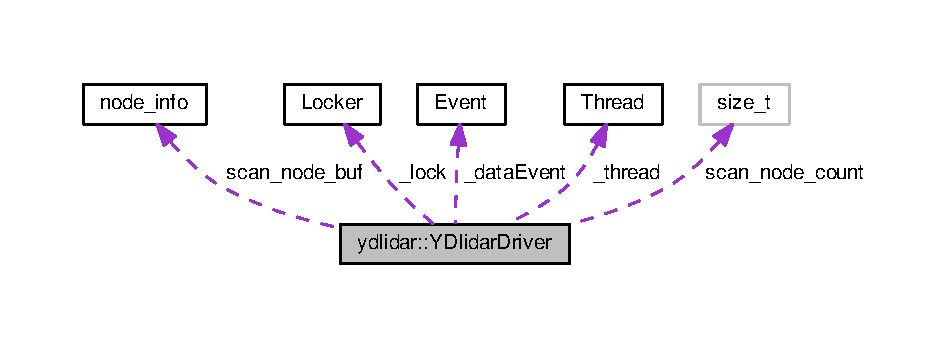
\includegraphics[width=350pt]{classydlidar_1_1_y_dlidar_driver__coll__graph}
\end{center}
\end{figure}
\subsection*{Public Types}
\begin{DoxyCompactItemize}
\item 
enum \{ \hyperlink{classydlidar_1_1_y_dlidar_driver_a13a4f2dc4067b43794b2c47c06d5d27aa07c79ce96f468ff4b40495ef84584442}{D\+E\+F\+A\+U\+L\+T\+\_\+\+T\+I\+M\+E\+O\+UT} = 2000, 
\hyperlink{classydlidar_1_1_y_dlidar_driver_a13a4f2dc4067b43794b2c47c06d5d27aa94033b4717c83f52cd008fe38b712e21}{D\+E\+F\+A\+U\+L\+T\+\_\+\+H\+E\+A\+R\+T\+\_\+\+B\+E\+AT} = 1000, 
\hyperlink{classydlidar_1_1_y_dlidar_driver_a13a4f2dc4067b43794b2c47c06d5d27aa3db6fc46c7ce55cdf3a968b70e96374a}{M\+A\+X\+\_\+\+S\+C\+A\+N\+\_\+\+N\+O\+D\+ES} = 2048
 \}
\item 
enum \{ \\*
\hyperlink{classydlidar_1_1_y_dlidar_driver_abbb612f1ac6a9f6dfdcfeafb149dd0daa3303d67e56b0dd5a36397a5326965713}{Y\+D\+L\+I\+D\+A\+R\+\_\+\+F4} =1, 
\hyperlink{classydlidar_1_1_y_dlidar_driver_abbb612f1ac6a9f6dfdcfeafb149dd0daa6ea5ed1cde351e4b5df40d1bbd697212}{Y\+D\+L\+I\+D\+A\+R\+\_\+\+T1} =2, 
\hyperlink{classydlidar_1_1_y_dlidar_driver_abbb612f1ac6a9f6dfdcfeafb149dd0daa7d64a3d3e3d3ef6d1db5c0a8740a523a}{Y\+D\+L\+I\+D\+A\+R\+\_\+\+F2} =3, 
\hyperlink{classydlidar_1_1_y_dlidar_driver_abbb612f1ac6a9f6dfdcfeafb149dd0daab1d9ab224053d610e97ebee7236345ba}{Y\+D\+L\+I\+D\+A\+R\+\_\+\+S4} =4, 
\\*
\hyperlink{classydlidar_1_1_y_dlidar_driver_abbb612f1ac6a9f6dfdcfeafb149dd0daa6bd6fb5e1f3ddd4e36ab12e53c114039}{Y\+D\+L\+I\+D\+A\+R\+\_\+\+G4} =5, 
\hyperlink{classydlidar_1_1_y_dlidar_driver_abbb612f1ac6a9f6dfdcfeafb149dd0daa5065807c3aa6a4a731858dda599667b7}{Y\+D\+L\+I\+D\+A\+R\+\_\+\+X4} =6, 
\hyperlink{classydlidar_1_1_y_dlidar_driver_abbb612f1ac6a9f6dfdcfeafb149dd0daa700fca9e58a191c0d1a4d13ae67927e8}{Y\+D\+L\+I\+D\+A\+R\+\_\+\+F4\+P\+RO} =6, 
\hyperlink{classydlidar_1_1_y_dlidar_driver_abbb612f1ac6a9f6dfdcfeafb149dd0daa55a9d7236d51f9d1d38d41cd102be527}{Y\+D\+L\+I\+D\+A\+R\+\_\+\+G4C} =9
 \}
\end{DoxyCompactItemize}
\subsection*{Public Member Functions}
\begin{DoxyCompactItemize}
\item 
result\+\_\+t \hyperlink{classydlidar_1_1_y_dlidar_driver_a2c5eeecccaa6ed874635de1617e8d7d8}{connect} (const char $\ast$port\+\_\+path, uint32\+\_\+t baudrate)
\begin{DoxyCompactList}\small\item\em 连接雷达 ~\newline
连接成功后,必须使用\+::disconnect函数关闭 \end{DoxyCompactList}\item 
void \hyperlink{classydlidar_1_1_y_dlidar_driver_aa26790ae49d33936229fa67739a8ff5f}{disconnect} ()\hypertarget{classydlidar_1_1_y_dlidar_driver_aa26790ae49d33936229fa67739a8ff5f}{}\label{classydlidar_1_1_y_dlidar_driver_aa26790ae49d33936229fa67739a8ff5f}

\begin{DoxyCompactList}\small\item\em 断开雷达连接 \end{DoxyCompactList}\item 
const bool \hyperlink{classydlidar_1_1_y_dlidar_driver_a37cd2766dec3536848aa25c88d9d1ea9}{isscanning} () const 
\begin{DoxyCompactList}\small\item\em 扫图状态 ~\newline
\end{DoxyCompactList}\item 
const bool \hyperlink{classydlidar_1_1_y_dlidar_driver_a2553d28304faa4acab6bd63e7c6c2ee6}{isconnected} () const 
\begin{DoxyCompactList}\small\item\em 连接雷达状态 ~\newline
\end{DoxyCompactList}\item 
void \hyperlink{classydlidar_1_1_y_dlidar_driver_afc543dbbe1c5e37afc366e3c92203533}{set\+Intensities} (const bool \&isintensities)
\begin{DoxyCompactList}\small\item\em 设置雷达是否带信号质量 ~\newline
连接成功后,必须使用\+::disconnect函数关闭 \end{DoxyCompactList}\item 
const bool \hyperlink{classydlidar_1_1_y_dlidar_driver_a36b01c5124032be12ecbeffeefd38742}{get\+Heart\+Beat} () const 
\begin{DoxyCompactList}\small\item\em 获取当前雷达掉电保护功能 ~\newline
\end{DoxyCompactList}\item 
void \hyperlink{classydlidar_1_1_y_dlidar_driver_af5d6603d3664d3efcb56d64d76d31956}{set\+Heart\+Beat} (const bool \&enable)
\begin{DoxyCompactList}\small\item\em 设置雷达掉电保护使能 ~\newline
\end{DoxyCompactList}\item 
result\+\_\+t \hyperlink{classydlidar_1_1_y_dlidar_driver_a9fe6f8b842a2aff2c3ae13f8423b03f4}{get\+Health} (\hyperlink{structdevice__health}{device\+\_\+health} \&health, uint32\+\_\+t timeout=\hyperlink{classydlidar_1_1_y_dlidar_driver_a13a4f2dc4067b43794b2c47c06d5d27aa07c79ce96f468ff4b40495ef84584442}{D\+E\+F\+A\+U\+L\+T\+\_\+\+T\+I\+M\+E\+O\+UT})
\begin{DoxyCompactList}\small\item\em 获取雷达设备健康状态 ~\newline
\end{DoxyCompactList}\item 
result\+\_\+t \hyperlink{classydlidar_1_1_y_dlidar_driver_ab75303116c4ccb144ecc215e94114e1a}{get\+Device\+Info} (\hyperlink{structdevice__info}{device\+\_\+info} \&info, uint32\+\_\+t timeout=\hyperlink{classydlidar_1_1_y_dlidar_driver_a13a4f2dc4067b43794b2c47c06d5d27aa07c79ce96f468ff4b40495ef84584442}{D\+E\+F\+A\+U\+L\+T\+\_\+\+T\+I\+M\+E\+O\+UT})
\begin{DoxyCompactList}\small\item\em 获取雷达设备信息 ~\newline
\end{DoxyCompactList}\item 
result\+\_\+t \hyperlink{classydlidar_1_1_y_dlidar_driver_a62888da8520422b7daaae89c2935460b}{start\+Scan} (bool force=false, uint32\+\_\+t timeout=\hyperlink{classydlidar_1_1_y_dlidar_driver_a13a4f2dc4067b43794b2c47c06d5d27aa07c79ce96f468ff4b40495ef84584442}{D\+E\+F\+A\+U\+L\+T\+\_\+\+T\+I\+M\+E\+O\+UT})
\begin{DoxyCompactList}\small\item\em 开启扫描 ~\newline
\end{DoxyCompactList}\item 
result\+\_\+t \hyperlink{classydlidar_1_1_y_dlidar_driver_a7aa354e88eeb6984be4d18eae6367a0b}{stop} ()
\begin{DoxyCompactList}\small\item\em 关闭扫描 ~\newline
\end{DoxyCompactList}\item 
result\+\_\+t \hyperlink{classydlidar_1_1_y_dlidar_driver_a6d6e04efa9d7e5d4aea41ee53d4ea8af}{grab\+Scan\+Data} (\hyperlink{structnode__info}{node\+\_\+info} $\ast$nodebuffer, size\+\_\+t \&count, uint32\+\_\+t timeout=\hyperlink{classydlidar_1_1_y_dlidar_driver_a13a4f2dc4067b43794b2c47c06d5d27aa07c79ce96f468ff4b40495ef84584442}{D\+E\+F\+A\+U\+L\+T\+\_\+\+T\+I\+M\+E\+O\+UT})
\begin{DoxyCompactList}\small\item\em 获取激光数据 ~\newline
\end{DoxyCompactList}\item 
result\+\_\+t \hyperlink{classydlidar_1_1_y_dlidar_driver_a6494501f3fee2f6dc410f869bbc18cb9}{ascend\+Scan\+Data} (\hyperlink{structnode__info}{node\+\_\+info} $\ast$nodebuffer, size\+\_\+t count)
\begin{DoxyCompactList}\small\item\em 补偿激光角度 ~\newline
把角度限制在0到360度之间 \end{DoxyCompactList}\item 
result\+\_\+t \hyperlink{classydlidar_1_1_y_dlidar_driver_a3dd4086c5685163f7c7487ea0f5af08c}{reset} (uint32\+\_\+t timeout=\hyperlink{classydlidar_1_1_y_dlidar_driver_a13a4f2dc4067b43794b2c47c06d5d27aa07c79ce96f468ff4b40495ef84584442}{D\+E\+F\+A\+U\+L\+T\+\_\+\+T\+I\+M\+E\+O\+UT})
\begin{DoxyCompactList}\small\item\em 重置激光雷达 ~\newline
\end{DoxyCompactList}\item 
result\+\_\+t \hyperlink{classydlidar_1_1_y_dlidar_driver_a2e686ef1ce60f3241352a798330f760b}{start\+Motor} ()
\begin{DoxyCompactList}\small\item\em 打开电机 ~\newline
\end{DoxyCompactList}\item 
result\+\_\+t \hyperlink{classydlidar_1_1_y_dlidar_driver_a6cdf0c5a7ddf2375c1392c3a0e65edfe}{stop\+Motor} ()
\begin{DoxyCompactList}\small\item\em 关闭电机 ~\newline
\end{DoxyCompactList}\item 
result\+\_\+t \hyperlink{classydlidar_1_1_y_dlidar_driver_a76efb701e137121b213f61028e3f235e}{get\+Scan\+Frequency} (\hyperlink{structscan__frequency}{scan\+\_\+frequency} \&frequency, uint32\+\_\+t timeout=\hyperlink{classydlidar_1_1_y_dlidar_driver_a13a4f2dc4067b43794b2c47c06d5d27aa07c79ce96f468ff4b40495ef84584442}{D\+E\+F\+A\+U\+L\+T\+\_\+\+T\+I\+M\+E\+O\+UT})
\begin{DoxyCompactList}\small\item\em 获取激光雷达当前扫描频率 ~\newline
\end{DoxyCompactList}\item 
result\+\_\+t \hyperlink{classydlidar_1_1_y_dlidar_driver_a0feea99573991bb4eb6f8e1718a71435}{set\+Scan\+Frequency\+Add} (\hyperlink{structscan__frequency}{scan\+\_\+frequency} \&frequency, uint32\+\_\+t timeout=\hyperlink{classydlidar_1_1_y_dlidar_driver_a13a4f2dc4067b43794b2c47c06d5d27aa07c79ce96f468ff4b40495ef84584442}{D\+E\+F\+A\+U\+L\+T\+\_\+\+T\+I\+M\+E\+O\+UT})
\begin{DoxyCompactList}\small\item\em 设置增加扫描频率1\+HZ ~\newline
\end{DoxyCompactList}\item 
result\+\_\+t \hyperlink{classydlidar_1_1_y_dlidar_driver_a811e3e1f0012925c8a90aebda9716738}{set\+Scan\+Frequency\+Dis} (\hyperlink{structscan__frequency}{scan\+\_\+frequency} \&frequency, uint32\+\_\+t timeout=\hyperlink{classydlidar_1_1_y_dlidar_driver_a13a4f2dc4067b43794b2c47c06d5d27aa07c79ce96f468ff4b40495ef84584442}{D\+E\+F\+A\+U\+L\+T\+\_\+\+T\+I\+M\+E\+O\+UT})
\begin{DoxyCompactList}\small\item\em 设置减小扫描频率1\+HZ ~\newline
\end{DoxyCompactList}\item 
result\+\_\+t \hyperlink{classydlidar_1_1_y_dlidar_driver_aa801f64f5ca2ce1e70ee096eb0b4b612}{set\+Scan\+Frequency\+Add\+Mic} (\hyperlink{structscan__frequency}{scan\+\_\+frequency} \&frequency, uint32\+\_\+t timeout=\hyperlink{classydlidar_1_1_y_dlidar_driver_a13a4f2dc4067b43794b2c47c06d5d27aa07c79ce96f468ff4b40495ef84584442}{D\+E\+F\+A\+U\+L\+T\+\_\+\+T\+I\+M\+E\+O\+UT})
\begin{DoxyCompactList}\small\item\em 设置增加扫描频率0.1\+HZ ~\newline
\end{DoxyCompactList}\item 
result\+\_\+t \hyperlink{classydlidar_1_1_y_dlidar_driver_a00e69cf360eeca890dbaf964ab6f67b7}{set\+Scan\+Frequency\+Dis\+Mic} (\hyperlink{structscan__frequency}{scan\+\_\+frequency} \&frequency, uint32\+\_\+t timeout=\hyperlink{classydlidar_1_1_y_dlidar_driver_a13a4f2dc4067b43794b2c47c06d5d27aa07c79ce96f468ff4b40495ef84584442}{D\+E\+F\+A\+U\+L\+T\+\_\+\+T\+I\+M\+E\+O\+UT})
\begin{DoxyCompactList}\small\item\em 设置减小扫描频率0.1\+HZ ~\newline
\end{DoxyCompactList}\item 
result\+\_\+t \hyperlink{classydlidar_1_1_y_dlidar_driver_a7b7812329013f119235abf74da397aaa}{get\+Sampling\+Rate} (\hyperlink{structsampling__rate}{sampling\+\_\+rate} \&rate, uint32\+\_\+t timeout=\hyperlink{classydlidar_1_1_y_dlidar_driver_a13a4f2dc4067b43794b2c47c06d5d27aa07c79ce96f468ff4b40495ef84584442}{D\+E\+F\+A\+U\+L\+T\+\_\+\+T\+I\+M\+E\+O\+UT})
\begin{DoxyCompactList}\small\item\em 获取激光雷达当前采样频率 ~\newline
\end{DoxyCompactList}\item 
result\+\_\+t \hyperlink{classydlidar_1_1_y_dlidar_driver_a30f9219bcf3aa3a8df2bbdae983ccd02}{set\+Sampling\+Rate} (\hyperlink{structsampling__rate}{sampling\+\_\+rate} \&rate, uint32\+\_\+t timeout=\hyperlink{classydlidar_1_1_y_dlidar_driver_a13a4f2dc4067b43794b2c47c06d5d27aa07c79ce96f468ff4b40495ef84584442}{D\+E\+F\+A\+U\+L\+T\+\_\+\+T\+I\+M\+E\+O\+UT})
\begin{DoxyCompactList}\small\item\em 设置激光雷达当前采样频率 ~\newline
\end{DoxyCompactList}\item 
result\+\_\+t \hyperlink{classydlidar_1_1_y_dlidar_driver_ae6645c26b9b46b2aa4aaae87521a38f1}{set\+Rotation\+Positive} (\hyperlink{structscan__rotation}{scan\+\_\+rotation} \&rotation, uint32\+\_\+t timeout=\hyperlink{classydlidar_1_1_y_dlidar_driver_a13a4f2dc4067b43794b2c47c06d5d27aa07c79ce96f468ff4b40495ef84584442}{D\+E\+F\+A\+U\+L\+T\+\_\+\+T\+I\+M\+E\+O\+UT})
\begin{DoxyCompactList}\small\item\em 设置电机顺时针旋转 ~\newline
\end{DoxyCompactList}\item 
result\+\_\+t \hyperlink{classydlidar_1_1_y_dlidar_driver_a1569723d0e46b801aee5284455f3b1d1}{set\+Rotation\+Inversion} (\hyperlink{structscan__rotation}{scan\+\_\+rotation} \&rotation, uint32\+\_\+t timeout=\hyperlink{classydlidar_1_1_y_dlidar_driver_a13a4f2dc4067b43794b2c47c06d5d27aa07c79ce96f468ff4b40495ef84584442}{D\+E\+F\+A\+U\+L\+T\+\_\+\+T\+I\+M\+E\+O\+UT})
\begin{DoxyCompactList}\small\item\em 设置电机逆顺时针旋转 ~\newline
\end{DoxyCompactList}\item 
result\+\_\+t \hyperlink{classydlidar_1_1_y_dlidar_driver_a85a9af2aff7201a42f000299990b0ce5}{enable\+Lower\+Power} (\hyperlink{structfunction__state}{function\+\_\+state} \&state, uint32\+\_\+t timeout=\hyperlink{classydlidar_1_1_y_dlidar_driver_a13a4f2dc4067b43794b2c47c06d5d27aa07c79ce96f468ff4b40495ef84584442}{D\+E\+F\+A\+U\+L\+T\+\_\+\+T\+I\+M\+E\+O\+UT})
\begin{DoxyCompactList}\small\item\em 低功耗使能 ~\newline
\end{DoxyCompactList}\item 
result\+\_\+t \hyperlink{classydlidar_1_1_y_dlidar_driver_a18895e94f42ce61890b4912727cdfbd8}{disable\+Lower\+Power} (\hyperlink{structfunction__state}{function\+\_\+state} \&state, uint32\+\_\+t timeout=\hyperlink{classydlidar_1_1_y_dlidar_driver_a13a4f2dc4067b43794b2c47c06d5d27aa07c79ce96f468ff4b40495ef84584442}{D\+E\+F\+A\+U\+L\+T\+\_\+\+T\+I\+M\+E\+O\+UT})
\begin{DoxyCompactList}\small\item\em 关闭低功耗 ~\newline
\end{DoxyCompactList}\item 
result\+\_\+t \hyperlink{classydlidar_1_1_y_dlidar_driver_af5d460ababe4b8a34b02d33268f24d4d}{get\+Motor\+State} (\hyperlink{structfunction__state}{function\+\_\+state} \&state, uint32\+\_\+t timeout=\hyperlink{classydlidar_1_1_y_dlidar_driver_a13a4f2dc4067b43794b2c47c06d5d27aa07c79ce96f468ff4b40495ef84584442}{D\+E\+F\+A\+U\+L\+T\+\_\+\+T\+I\+M\+E\+O\+UT})
\begin{DoxyCompactList}\small\item\em 获取电机状态 ~\newline
\end{DoxyCompactList}\item 
result\+\_\+t \hyperlink{classydlidar_1_1_y_dlidar_driver_a1e5c25618be9867dfdb1aa2f5e9cb93c}{enable\+Const\+Freq} (\hyperlink{structfunction__state}{function\+\_\+state} \&state, uint32\+\_\+t timeout=\hyperlink{classydlidar_1_1_y_dlidar_driver_a13a4f2dc4067b43794b2c47c06d5d27aa07c79ce96f468ff4b40495ef84584442}{D\+E\+F\+A\+U\+L\+T\+\_\+\+T\+I\+M\+E\+O\+UT})
\begin{DoxyCompactList}\small\item\em 开启恒频功能 ~\newline
\end{DoxyCompactList}\item 
result\+\_\+t \hyperlink{classydlidar_1_1_y_dlidar_driver_ae4b3883dd18bf01737bc4783d2dae974}{disable\+Const\+Freq} (\hyperlink{structfunction__state}{function\+\_\+state} \&state, uint32\+\_\+t timeout=\hyperlink{classydlidar_1_1_y_dlidar_driver_a13a4f2dc4067b43794b2c47c06d5d27aa07c79ce96f468ff4b40495ef84584442}{D\+E\+F\+A\+U\+L\+T\+\_\+\+T\+I\+M\+E\+O\+UT})
\begin{DoxyCompactList}\small\item\em 关闭恒频功能 ~\newline
\end{DoxyCompactList}\item 
result\+\_\+t \hyperlink{classydlidar_1_1_y_dlidar_driver_a73ef6628afc1eadf2f3079db99b383c6}{set\+Save\+Low\+Exposure} (\hyperlink{structscan__exposure}{scan\+\_\+exposure} \&low\+\_\+exposure, uint32\+\_\+t timeout=\hyperlink{classydlidar_1_1_y_dlidar_driver_a13a4f2dc4067b43794b2c47c06d5d27aa07c79ce96f468ff4b40495ef84584442}{D\+E\+F\+A\+U\+L\+T\+\_\+\+T\+I\+M\+E\+O\+UT})
\begin{DoxyCompactList}\small\item\em 保存当前激光曝光值 ~\newline
\end{DoxyCompactList}\item 
result\+\_\+t \hyperlink{classydlidar_1_1_y_dlidar_driver_a02257e37b792870a9c42f8abfbe543ad}{set\+Low\+Exposure} (\hyperlink{structscan__exposure}{scan\+\_\+exposure} \&low\+\_\+exposure, uint32\+\_\+t timeout=\hyperlink{classydlidar_1_1_y_dlidar_driver_a13a4f2dc4067b43794b2c47c06d5d27aa07c79ce96f468ff4b40495ef84584442}{D\+E\+F\+A\+U\+L\+T\+\_\+\+T\+I\+M\+E\+O\+UT})
\begin{DoxyCompactList}\small\item\em 设置低光功率模式 ~\newline
\end{DoxyCompactList}\item 
result\+\_\+t \hyperlink{classydlidar_1_1_y_dlidar_driver_a3f34ad1119b9b97c4af3936e80c182f4}{set\+Low\+Exposure\+Add} (\hyperlink{structscan__exposure}{scan\+\_\+exposure} \&exposure, uint32\+\_\+t timeout=\hyperlink{classydlidar_1_1_y_dlidar_driver_a13a4f2dc4067b43794b2c47c06d5d27aa07c79ce96f468ff4b40495ef84584442}{D\+E\+F\+A\+U\+L\+T\+\_\+\+T\+I\+M\+E\+O\+UT})
\begin{DoxyCompactList}\small\item\em 增加激光曝光值 ~\newline
\end{DoxyCompactList}\item 
result\+\_\+t \hyperlink{classydlidar_1_1_y_dlidar_driver_aece83871e5912d19bc7677676a5511f8}{set\+Low\+Exposurer\+Dis} (\hyperlink{structscan__exposure}{scan\+\_\+exposure} \&exposure, uint32\+\_\+t timeout=\hyperlink{classydlidar_1_1_y_dlidar_driver_a13a4f2dc4067b43794b2c47c06d5d27aa07c79ce96f468ff4b40495ef84584442}{D\+E\+F\+A\+U\+L\+T\+\_\+\+T\+I\+M\+E\+O\+UT})
\begin{DoxyCompactList}\small\item\em 减小激光曝光值 ~\newline
\end{DoxyCompactList}\item 
result\+\_\+t \hyperlink{classydlidar_1_1_y_dlidar_driver_ab2d5434c9b640a38f9d3b43b07c0b3eb}{set\+Scan\+Heartbeat} (\hyperlink{structscan__heart__beat}{scan\+\_\+heart\+\_\+beat} \&beat, uint32\+\_\+t timeout=\hyperlink{classydlidar_1_1_y_dlidar_driver_a13a4f2dc4067b43794b2c47c06d5d27aa07c79ce96f468ff4b40495ef84584442}{D\+E\+F\+A\+U\+L\+T\+\_\+\+T\+I\+M\+E\+O\+UT})
\begin{DoxyCompactList}\small\item\em 设置雷达掉电保护状态 ~\newline
\end{DoxyCompactList}\item 
result\+\_\+t \hyperlink{classydlidar_1_1_y_dlidar_driver_a1c8d40889885386e6c5a7827b7747696}{set\+Points\+For\+One\+Ring\+Flag} (\hyperlink{structscan__points}{scan\+\_\+points} \&points, uint32\+\_\+t timeout=\hyperlink{classydlidar_1_1_y_dlidar_driver_a13a4f2dc4067b43794b2c47c06d5d27aa07c79ce96f468ff4b40495ef84584442}{D\+E\+F\+A\+U\+L\+T\+\_\+\+T\+I\+M\+E\+O\+UT})
\begin{DoxyCompactList}\small\item\em 设置扫描一圈固定激光点数 ~\newline
\end{DoxyCompactList}\item 
void \hyperlink{classydlidar_1_1_y_dlidar_driver_a797de2678c6c81c84a8126cf184a0254}{simple\+Scan\+Data} (std\+::vector$<$ \hyperlink{structscan_dot}{scan\+Dot} $>$ $\ast$scan\+\_\+data, \hyperlink{structnode__info}{node\+\_\+info} $\ast$buffer, size\+\_\+t count)
\begin{DoxyCompactList}\small\item\em 解析激光信息数据到scan\+Dot数据类型 ~\newline
\end{DoxyCompactList}\end{DoxyCompactItemize}
\subsection*{Static Public Member Functions}
\begin{DoxyCompactItemize}
\item 
static \hyperlink{classydlidar_1_1_y_dlidar_driver}{Y\+Dlidar\+Driver} $\ast$ {\bfseries singleton} ()\hypertarget{classydlidar_1_1_y_dlidar_driver_ae647504b6232c8fce584ca2d011a07d3}{}\label{classydlidar_1_1_y_dlidar_driver_ae647504b6232c8fce584ca2d011a07d3}

\item 
static void {\bfseries init\+Driver} ()\hypertarget{classydlidar_1_1_y_dlidar_driver_a15629ca7d39a463d1b18a5e35300dfe7}{}\label{classydlidar_1_1_y_dlidar_driver_a15629ca7d39a463d1b18a5e35300dfe7}

\item 
static void {\bfseries done} ()\hypertarget{classydlidar_1_1_y_dlidar_driver_a167ea8a27d77fae98488f1ba7f31969c}{}\label{classydlidar_1_1_y_dlidar_driver_a167ea8a27d77fae98488f1ba7f31969c}

\item 
static std\+::string \hyperlink{classydlidar_1_1_y_dlidar_driver_a542dc18ac8dbcda2a51657cf9bd44ae0}{get\+S\+D\+K\+Version} ()
\begin{DoxyCompactList}\small\item\em 获取当前\+S\+D\+K版本号 ~\newline
静态函数 \end{DoxyCompactList}\end{DoxyCompactItemize}
\subsection*{Public Attributes}
\begin{DoxyCompactItemize}
\item 
std\+::atomic$<$ bool $>$ \hyperlink{classydlidar_1_1_y_dlidar_driver_a4457578961d36ce22035d778c0fd7f06}{is\+Connected}\hypertarget{classydlidar_1_1_y_dlidar_driver_a4457578961d36ce22035d778c0fd7f06}{}\label{classydlidar_1_1_y_dlidar_driver_a4457578961d36ce22035d778c0fd7f06}

\begin{DoxyCompactList}\small\item\em 串口连接状体 \end{DoxyCompactList}\item 
std\+::atomic$<$ bool $>$ \hyperlink{classydlidar_1_1_y_dlidar_driver_a245115a8c8a4f98d988fbee06810d0a4}{is\+Scanning}\hypertarget{classydlidar_1_1_y_dlidar_driver_a245115a8c8a4f98d988fbee06810d0a4}{}\label{classydlidar_1_1_y_dlidar_driver_a245115a8c8a4f98d988fbee06810d0a4}

\begin{DoxyCompactList}\small\item\em 扫图状态 \end{DoxyCompactList}\item 
std\+::atomic$<$ bool $>$ \hyperlink{classydlidar_1_1_y_dlidar_driver_a8a57494e849e7735fe8bf46d00b63077}{is\+Heartbeat}\hypertarget{classydlidar_1_1_y_dlidar_driver_a8a57494e849e7735fe8bf46d00b63077}{}\label{classydlidar_1_1_y_dlidar_driver_a8a57494e849e7735fe8bf46d00b63077}

\begin{DoxyCompactList}\small\item\em 掉电保护状态 \end{DoxyCompactList}\item 
\hyperlink{structnode__info}{node\+\_\+info} \hyperlink{classydlidar_1_1_y_dlidar_driver_aeaefa47c69cbb0439b1259bdc6ccb29e}{scan\+\_\+node\+\_\+buf} \mbox{[}2048\mbox{]}\hypertarget{classydlidar_1_1_y_dlidar_driver_aeaefa47c69cbb0439b1259bdc6ccb29e}{}\label{classydlidar_1_1_y_dlidar_driver_aeaefa47c69cbb0439b1259bdc6ccb29e}

\begin{DoxyCompactList}\small\item\em 激光点信息 \end{DoxyCompactList}\item 
size\+\_\+t \hyperlink{classydlidar_1_1_y_dlidar_driver_a106fc563bb42f19e84e8d9db1e7856fe}{scan\+\_\+node\+\_\+count}\hypertarget{classydlidar_1_1_y_dlidar_driver_a106fc563bb42f19e84e8d9db1e7856fe}{}\label{classydlidar_1_1_y_dlidar_driver_a106fc563bb42f19e84e8d9db1e7856fe}

\begin{DoxyCompactList}\small\item\em 激光点数 \end{DoxyCompactList}\item 
\hyperlink{class_event}{Event} \hyperlink{classydlidar_1_1_y_dlidar_driver_afd2b3835a0e450d9b88d28d8f574148d}{\+\_\+data\+Event}\hypertarget{classydlidar_1_1_y_dlidar_driver_afd2b3835a0e450d9b88d28d8f574148d}{}\label{classydlidar_1_1_y_dlidar_driver_afd2b3835a0e450d9b88d28d8f574148d}

\begin{DoxyCompactList}\small\item\em 数据同步事件 \end{DoxyCompactList}\item 
\hyperlink{class_locker}{Locker} \hyperlink{classydlidar_1_1_y_dlidar_driver_a1bb836661c8c39c2b71c9a0de8755c5c}{\+\_\+lock}\hypertarget{classydlidar_1_1_y_dlidar_driver_a1bb836661c8c39c2b71c9a0de8755c5c}{}\label{classydlidar_1_1_y_dlidar_driver_a1bb836661c8c39c2b71c9a0de8755c5c}

\begin{DoxyCompactList}\small\item\em 线程锁 \end{DoxyCompactList}\item 
\hyperlink{class_thread}{Thread} \hyperlink{classydlidar_1_1_y_dlidar_driver_a9fbd1b3471c1aa4959d74524b9a92410}{\+\_\+thread}\hypertarget{classydlidar_1_1_y_dlidar_driver_a9fbd1b3471c1aa4959d74524b9a92410}{}\label{classydlidar_1_1_y_dlidar_driver_a9fbd1b3471c1aa4959d74524b9a92410}

\begin{DoxyCompactList}\small\item\em 线程id \end{DoxyCompactList}\end{DoxyCompactItemize}
\subsection*{Protected Member Functions}
\begin{DoxyCompactItemize}
\item 
\hyperlink{classydlidar_1_1_y_dlidar_driver_a19e20b6aa35834507a0dacc8a3c510e6}{Y\+Dlidar\+Driver} ()
\item 
virtual \hyperlink{classydlidar_1_1_y_dlidar_driver_a87a50f9f1093a93b4d985f3e8bf27fde}{$\sim$\+Y\+Dlidar\+Driver} ()
\item 
result\+\_\+t \hyperlink{classydlidar_1_1_y_dlidar_driver_a2d2b317fa6381009222e03670812e917}{create\+Thread} ()
\begin{DoxyCompactList}\small\item\em 创建解析雷达数据线程 ~\newline
\end{DoxyCompactList}\item 
result\+\_\+t \hyperlink{classydlidar_1_1_y_dlidar_driver_aaf78903693f58c7f739dfa493573b3b1}{wait\+Package} (\hyperlink{structnode__info}{node\+\_\+info} $\ast$node, uint32\+\_\+t timeout=\hyperlink{classydlidar_1_1_y_dlidar_driver_a13a4f2dc4067b43794b2c47c06d5d27aa07c79ce96f468ff4b40495ef84584442}{D\+E\+F\+A\+U\+L\+T\+\_\+\+T\+I\+M\+E\+O\+UT})
\begin{DoxyCompactList}\small\item\em 解包激光数据 ~\newline
\end{DoxyCompactList}\item 
result\+\_\+t \hyperlink{classydlidar_1_1_y_dlidar_driver_a574996217284ce34191a2f3675a9f17b}{wait\+Scan\+Data} (\hyperlink{structnode__info}{node\+\_\+info} $\ast$nodebuffer, size\+\_\+t \&count, uint32\+\_\+t timeout=\hyperlink{classydlidar_1_1_y_dlidar_driver_a13a4f2dc4067b43794b2c47c06d5d27aa07c79ce96f468ff4b40495ef84584442}{D\+E\+F\+A\+U\+L\+T\+\_\+\+T\+I\+M\+E\+O\+UT})
\begin{DoxyCompactList}\small\item\em 发送数据到雷达 ~\newline
\end{DoxyCompactList}\item 
int \hyperlink{classydlidar_1_1_y_dlidar_driver_ab462b22dc3a4d39fef4f722345a87d5e}{cache\+Scan\+Data} ()\hypertarget{classydlidar_1_1_y_dlidar_driver_ab462b22dc3a4d39fef4f722345a87d5e}{}\label{classydlidar_1_1_y_dlidar_driver_ab462b22dc3a4d39fef4f722345a87d5e}

\begin{DoxyCompactList}\small\item\em 激光数据解析线程 ~\newline
\end{DoxyCompactList}\item 
result\+\_\+t \hyperlink{classydlidar_1_1_y_dlidar_driver_ab096ecdc3642c04e3e8b000e210c0962}{send\+Command} (uint8\+\_\+t cmd, const void $\ast$payload=N\+U\+LL, size\+\_\+t payloadsize=0)
\begin{DoxyCompactList}\small\item\em 发送数据到雷达 ~\newline
\end{DoxyCompactList}\item 
result\+\_\+t \hyperlink{classydlidar_1_1_y_dlidar_driver_a0e089d615193ccef4bf488f63ff8130e}{wait\+Response\+Header} (\hyperlink{structlidar__ans__header}{lidar\+\_\+ans\+\_\+header} $\ast$header, uint32\+\_\+t timeout=\hyperlink{classydlidar_1_1_y_dlidar_driver_a13a4f2dc4067b43794b2c47c06d5d27aa07c79ce96f468ff4b40495ef84584442}{D\+E\+F\+A\+U\+L\+T\+\_\+\+T\+I\+M\+E\+O\+UT})
\begin{DoxyCompactList}\small\item\em 等待激光数据包头 ~\newline
\end{DoxyCompactList}\item 
result\+\_\+t \hyperlink{classydlidar_1_1_y_dlidar_driver_a13f404b44f51941d1642bfe250de3522}{wait\+For\+Data} (size\+\_\+t data\+\_\+count, uint32\+\_\+t timeout=\hyperlink{classydlidar_1_1_y_dlidar_driver_a13a4f2dc4067b43794b2c47c06d5d27aa07c79ce96f468ff4b40495ef84584442}{D\+E\+F\+A\+U\+L\+T\+\_\+\+T\+I\+M\+E\+O\+UT}, size\+\_\+t $\ast$returned\+\_\+size=N\+U\+LL)
\begin{DoxyCompactList}\small\item\em 等待固定数量串口数据 ~\newline
\end{DoxyCompactList}\item 
result\+\_\+t \hyperlink{classydlidar_1_1_y_dlidar_driver_ad787e714bc05e5a70a42b096e632c60f}{get\+Data} (uint8\+\_\+t $\ast$data, size\+\_\+t size)
\begin{DoxyCompactList}\small\item\em 获取串口数据 ~\newline
\end{DoxyCompactList}\item 
result\+\_\+t \hyperlink{classydlidar_1_1_y_dlidar_driver_a998ba4b05927d19e8a0d4d29d3d47656}{send\+Data} (const uint8\+\_\+t $\ast$data, size\+\_\+t size)
\begin{DoxyCompactList}\small\item\em 串口发送数据 ~\newline
\end{DoxyCompactList}\item 
result\+\_\+t \hyperlink{classydlidar_1_1_y_dlidar_driver_a6e7dc7cd2a73d24a763cebde840a5d30}{send\+Heart\+Beat} ()
\begin{DoxyCompactList}\small\item\em 发送掉电保护命令 ~\newline
\end{DoxyCompactList}\item 
void \hyperlink{classydlidar_1_1_y_dlidar_driver_ae66565bee3cdb8b74698b691f2ab1e63}{disable\+Data\+Grabbing} ()\hypertarget{classydlidar_1_1_y_dlidar_driver_ae66565bee3cdb8b74698b691f2ab1e63}{}\label{classydlidar_1_1_y_dlidar_driver_ae66565bee3cdb8b74698b691f2ab1e63}

\begin{DoxyCompactList}\small\item\em 关闭数据获取通道 ~\newline
\end{DoxyCompactList}\item 
void \hyperlink{classydlidar_1_1_y_dlidar_driver_a88de43cf13058344fc83389cb9df7e21}{set\+D\+TR} ()\hypertarget{classydlidar_1_1_y_dlidar_driver_a88de43cf13058344fc83389cb9df7e21}{}\label{classydlidar_1_1_y_dlidar_driver_a88de43cf13058344fc83389cb9df7e21}

\begin{DoxyCompactList}\small\item\em 设置串口\+D\+TR ~\newline
\end{DoxyCompactList}\item 
void \hyperlink{classydlidar_1_1_y_dlidar_driver_a67fe00d7458cdb52b4160d745b8ecd32}{clear\+D\+TR} ()\hypertarget{classydlidar_1_1_y_dlidar_driver_a67fe00d7458cdb52b4160d745b8ecd32}{}\label{classydlidar_1_1_y_dlidar_driver_a67fe00d7458cdb52b4160d745b8ecd32}

\begin{DoxyCompactList}\small\item\em 清除串口\+D\+TR ~\newline
\end{DoxyCompactList}\end{DoxyCompactItemize}


\subsection{Member Enumeration Documentation}
\subsubsection[{\texorpdfstring{anonymous enum}{anonymous enum}}]{\setlength{\rightskip}{0pt plus 5cm}anonymous enum}\hypertarget{classydlidar_1_1_y_dlidar_driver_a13a4f2dc4067b43794b2c47c06d5d27a}{}\label{classydlidar_1_1_y_dlidar_driver_a13a4f2dc4067b43794b2c47c06d5d27a}
\begin{Desc}
\item[Enumerator]\par
\begin{description}
\index{D\+E\+F\+A\+U\+L\+T\+\_\+\+T\+I\+M\+E\+O\+UT@{D\+E\+F\+A\+U\+L\+T\+\_\+\+T\+I\+M\+E\+O\+UT}!ydlidar\+::\+Y\+Dlidar\+Driver@{ydlidar\+::\+Y\+Dlidar\+Driver}}\index{ydlidar\+::\+Y\+Dlidar\+Driver@{ydlidar\+::\+Y\+Dlidar\+Driver}!D\+E\+F\+A\+U\+L\+T\+\_\+\+T\+I\+M\+E\+O\+UT@{D\+E\+F\+A\+U\+L\+T\+\_\+\+T\+I\+M\+E\+O\+UT}}\item[{\em 
D\+E\+F\+A\+U\+L\+T\+\_\+\+T\+I\+M\+E\+O\+UT\hypertarget{classydlidar_1_1_y_dlidar_driver_a13a4f2dc4067b43794b2c47c06d5d27aa07c79ce96f468ff4b40495ef84584442}{}\label{classydlidar_1_1_y_dlidar_driver_a13a4f2dc4067b43794b2c47c06d5d27aa07c79ce96f468ff4b40495ef84584442}
}]默认超时时间. \index{D\+E\+F\+A\+U\+L\+T\+\_\+\+H\+E\+A\+R\+T\+\_\+\+B\+E\+AT@{D\+E\+F\+A\+U\+L\+T\+\_\+\+H\+E\+A\+R\+T\+\_\+\+B\+E\+AT}!ydlidar\+::\+Y\+Dlidar\+Driver@{ydlidar\+::\+Y\+Dlidar\+Driver}}\index{ydlidar\+::\+Y\+Dlidar\+Driver@{ydlidar\+::\+Y\+Dlidar\+Driver}!D\+E\+F\+A\+U\+L\+T\+\_\+\+H\+E\+A\+R\+T\+\_\+\+B\+E\+AT@{D\+E\+F\+A\+U\+L\+T\+\_\+\+H\+E\+A\+R\+T\+\_\+\+B\+E\+AT}}\item[{\em 
D\+E\+F\+A\+U\+L\+T\+\_\+\+H\+E\+A\+R\+T\+\_\+\+B\+E\+AT\hypertarget{classydlidar_1_1_y_dlidar_driver_a13a4f2dc4067b43794b2c47c06d5d27aa94033b4717c83f52cd008fe38b712e21}{}\label{classydlidar_1_1_y_dlidar_driver_a13a4f2dc4067b43794b2c47c06d5d27aa94033b4717c83f52cd008fe38b712e21}
}]默认检测掉电功能时间. \index{M\+A\+X\+\_\+\+S\+C\+A\+N\+\_\+\+N\+O\+D\+ES@{M\+A\+X\+\_\+\+S\+C\+A\+N\+\_\+\+N\+O\+D\+ES}!ydlidar\+::\+Y\+Dlidar\+Driver@{ydlidar\+::\+Y\+Dlidar\+Driver}}\index{ydlidar\+::\+Y\+Dlidar\+Driver@{ydlidar\+::\+Y\+Dlidar\+Driver}!M\+A\+X\+\_\+\+S\+C\+A\+N\+\_\+\+N\+O\+D\+ES@{M\+A\+X\+\_\+\+S\+C\+A\+N\+\_\+\+N\+O\+D\+ES}}\item[{\em 
M\+A\+X\+\_\+\+S\+C\+A\+N\+\_\+\+N\+O\+D\+ES\hypertarget{classydlidar_1_1_y_dlidar_driver_a13a4f2dc4067b43794b2c47c06d5d27aa3db6fc46c7ce55cdf3a968b70e96374a}{}\label{classydlidar_1_1_y_dlidar_driver_a13a4f2dc4067b43794b2c47c06d5d27aa3db6fc46c7ce55cdf3a968b70e96374a}
}]最大扫描点数. \end{description}
\end{Desc}
\subsubsection[{\texorpdfstring{anonymous enum}{anonymous enum}}]{\setlength{\rightskip}{0pt plus 5cm}anonymous enum}\hypertarget{classydlidar_1_1_y_dlidar_driver_abbb612f1ac6a9f6dfdcfeafb149dd0da}{}\label{classydlidar_1_1_y_dlidar_driver_abbb612f1ac6a9f6dfdcfeafb149dd0da}
\begin{Desc}
\item[Enumerator]\par
\begin{description}
\index{Y\+D\+L\+I\+D\+A\+R\+\_\+\+F4@{Y\+D\+L\+I\+D\+A\+R\+\_\+\+F4}!ydlidar\+::\+Y\+Dlidar\+Driver@{ydlidar\+::\+Y\+Dlidar\+Driver}}\index{ydlidar\+::\+Y\+Dlidar\+Driver@{ydlidar\+::\+Y\+Dlidar\+Driver}!Y\+D\+L\+I\+D\+A\+R\+\_\+\+F4@{Y\+D\+L\+I\+D\+A\+R\+\_\+\+F4}}\item[{\em 
Y\+D\+L\+I\+D\+A\+R\+\_\+\+F4\hypertarget{classydlidar_1_1_y_dlidar_driver_abbb612f1ac6a9f6dfdcfeafb149dd0daa3303d67e56b0dd5a36397a5326965713}{}\label{classydlidar_1_1_y_dlidar_driver_abbb612f1ac6a9f6dfdcfeafb149dd0daa3303d67e56b0dd5a36397a5326965713}
}]F4雷达型号代号. \index{Y\+D\+L\+I\+D\+A\+R\+\_\+\+T1@{Y\+D\+L\+I\+D\+A\+R\+\_\+\+T1}!ydlidar\+::\+Y\+Dlidar\+Driver@{ydlidar\+::\+Y\+Dlidar\+Driver}}\index{ydlidar\+::\+Y\+Dlidar\+Driver@{ydlidar\+::\+Y\+Dlidar\+Driver}!Y\+D\+L\+I\+D\+A\+R\+\_\+\+T1@{Y\+D\+L\+I\+D\+A\+R\+\_\+\+T1}}\item[{\em 
Y\+D\+L\+I\+D\+A\+R\+\_\+\+T1\hypertarget{classydlidar_1_1_y_dlidar_driver_abbb612f1ac6a9f6dfdcfeafb149dd0daa6ea5ed1cde351e4b5df40d1bbd697212}{}\label{classydlidar_1_1_y_dlidar_driver_abbb612f1ac6a9f6dfdcfeafb149dd0daa6ea5ed1cde351e4b5df40d1bbd697212}
}]T1雷达型号代号. \index{Y\+D\+L\+I\+D\+A\+R\+\_\+\+F2@{Y\+D\+L\+I\+D\+A\+R\+\_\+\+F2}!ydlidar\+::\+Y\+Dlidar\+Driver@{ydlidar\+::\+Y\+Dlidar\+Driver}}\index{ydlidar\+::\+Y\+Dlidar\+Driver@{ydlidar\+::\+Y\+Dlidar\+Driver}!Y\+D\+L\+I\+D\+A\+R\+\_\+\+F2@{Y\+D\+L\+I\+D\+A\+R\+\_\+\+F2}}\item[{\em 
Y\+D\+L\+I\+D\+A\+R\+\_\+\+F2\hypertarget{classydlidar_1_1_y_dlidar_driver_abbb612f1ac6a9f6dfdcfeafb149dd0daa7d64a3d3e3d3ef6d1db5c0a8740a523a}{}\label{classydlidar_1_1_y_dlidar_driver_abbb612f1ac6a9f6dfdcfeafb149dd0daa7d64a3d3e3d3ef6d1db5c0a8740a523a}
}]F2雷达型号代号. \index{Y\+D\+L\+I\+D\+A\+R\+\_\+\+S4@{Y\+D\+L\+I\+D\+A\+R\+\_\+\+S4}!ydlidar\+::\+Y\+Dlidar\+Driver@{ydlidar\+::\+Y\+Dlidar\+Driver}}\index{ydlidar\+::\+Y\+Dlidar\+Driver@{ydlidar\+::\+Y\+Dlidar\+Driver}!Y\+D\+L\+I\+D\+A\+R\+\_\+\+S4@{Y\+D\+L\+I\+D\+A\+R\+\_\+\+S4}}\item[{\em 
Y\+D\+L\+I\+D\+A\+R\+\_\+\+S4\hypertarget{classydlidar_1_1_y_dlidar_driver_abbb612f1ac6a9f6dfdcfeafb149dd0daab1d9ab224053d610e97ebee7236345ba}{}\label{classydlidar_1_1_y_dlidar_driver_abbb612f1ac6a9f6dfdcfeafb149dd0daab1d9ab224053d610e97ebee7236345ba}
}]S4雷达型号代号. \index{Y\+D\+L\+I\+D\+A\+R\+\_\+\+G4@{Y\+D\+L\+I\+D\+A\+R\+\_\+\+G4}!ydlidar\+::\+Y\+Dlidar\+Driver@{ydlidar\+::\+Y\+Dlidar\+Driver}}\index{ydlidar\+::\+Y\+Dlidar\+Driver@{ydlidar\+::\+Y\+Dlidar\+Driver}!Y\+D\+L\+I\+D\+A\+R\+\_\+\+G4@{Y\+D\+L\+I\+D\+A\+R\+\_\+\+G4}}\item[{\em 
Y\+D\+L\+I\+D\+A\+R\+\_\+\+G4\hypertarget{classydlidar_1_1_y_dlidar_driver_abbb612f1ac6a9f6dfdcfeafb149dd0daa6bd6fb5e1f3ddd4e36ab12e53c114039}{}\label{classydlidar_1_1_y_dlidar_driver_abbb612f1ac6a9f6dfdcfeafb149dd0daa6bd6fb5e1f3ddd4e36ab12e53c114039}
}]G4雷达型号代号. \index{Y\+D\+L\+I\+D\+A\+R\+\_\+\+X4@{Y\+D\+L\+I\+D\+A\+R\+\_\+\+X4}!ydlidar\+::\+Y\+Dlidar\+Driver@{ydlidar\+::\+Y\+Dlidar\+Driver}}\index{ydlidar\+::\+Y\+Dlidar\+Driver@{ydlidar\+::\+Y\+Dlidar\+Driver}!Y\+D\+L\+I\+D\+A\+R\+\_\+\+X4@{Y\+D\+L\+I\+D\+A\+R\+\_\+\+X4}}\item[{\em 
Y\+D\+L\+I\+D\+A\+R\+\_\+\+X4\hypertarget{classydlidar_1_1_y_dlidar_driver_abbb612f1ac6a9f6dfdcfeafb149dd0daa5065807c3aa6a4a731858dda599667b7}{}\label{classydlidar_1_1_y_dlidar_driver_abbb612f1ac6a9f6dfdcfeafb149dd0daa5065807c3aa6a4a731858dda599667b7}
}]X4雷达型号代号. \index{Y\+D\+L\+I\+D\+A\+R\+\_\+\+F4\+P\+RO@{Y\+D\+L\+I\+D\+A\+R\+\_\+\+F4\+P\+RO}!ydlidar\+::\+Y\+Dlidar\+Driver@{ydlidar\+::\+Y\+Dlidar\+Driver}}\index{ydlidar\+::\+Y\+Dlidar\+Driver@{ydlidar\+::\+Y\+Dlidar\+Driver}!Y\+D\+L\+I\+D\+A\+R\+\_\+\+F4\+P\+RO@{Y\+D\+L\+I\+D\+A\+R\+\_\+\+F4\+P\+RO}}\item[{\em 
Y\+D\+L\+I\+D\+A\+R\+\_\+\+F4\+P\+RO\hypertarget{classydlidar_1_1_y_dlidar_driver_abbb612f1ac6a9f6dfdcfeafb149dd0daa700fca9e58a191c0d1a4d13ae67927e8}{}\label{classydlidar_1_1_y_dlidar_driver_abbb612f1ac6a9f6dfdcfeafb149dd0daa700fca9e58a191c0d1a4d13ae67927e8}
}]F4\+P\+R\+O雷达型号代号. \index{Y\+D\+L\+I\+D\+A\+R\+\_\+\+G4C@{Y\+D\+L\+I\+D\+A\+R\+\_\+\+G4C}!ydlidar\+::\+Y\+Dlidar\+Driver@{ydlidar\+::\+Y\+Dlidar\+Driver}}\index{ydlidar\+::\+Y\+Dlidar\+Driver@{ydlidar\+::\+Y\+Dlidar\+Driver}!Y\+D\+L\+I\+D\+A\+R\+\_\+\+G4C@{Y\+D\+L\+I\+D\+A\+R\+\_\+\+G4C}}\item[{\em 
Y\+D\+L\+I\+D\+A\+R\+\_\+\+G4C\hypertarget{classydlidar_1_1_y_dlidar_driver_abbb612f1ac6a9f6dfdcfeafb149dd0daa55a9d7236d51f9d1d38d41cd102be527}{}\label{classydlidar_1_1_y_dlidar_driver_abbb612f1ac6a9f6dfdcfeafb149dd0daa55a9d7236d51f9d1d38d41cd102be527}
}]G4\+C雷达型号代号. \end{description}
\end{Desc}


\subsection{Constructor \& Destructor Documentation}
\index{ydlidar\+::\+Y\+Dlidar\+Driver@{ydlidar\+::\+Y\+Dlidar\+Driver}!Y\+Dlidar\+Driver@{Y\+Dlidar\+Driver}}
\index{Y\+Dlidar\+Driver@{Y\+Dlidar\+Driver}!ydlidar\+::\+Y\+Dlidar\+Driver@{ydlidar\+::\+Y\+Dlidar\+Driver}}
\subsubsection[{\texorpdfstring{Y\+Dlidar\+Driver()}{YDlidarDriver()}}]{\setlength{\rightskip}{0pt plus 5cm}ydlidar\+::\+Y\+Dlidar\+Driver\+::\+Y\+Dlidar\+Driver (
\begin{DoxyParamCaption}
{}
\end{DoxyParamCaption}
)\hspace{0.3cm}{\ttfamily [protected]}}\hypertarget{classydlidar_1_1_y_dlidar_driver_a19e20b6aa35834507a0dacc8a3c510e6}{}\label{classydlidar_1_1_y_dlidar_driver_a19e20b6aa35834507a0dacc8a3c510e6}
A constructor. A more elaborate description of the constructor. \index{ydlidar\+::\+Y\+Dlidar\+Driver@{ydlidar\+::\+Y\+Dlidar\+Driver}!````~Y\+Dlidar\+Driver@{$\sim$\+Y\+Dlidar\+Driver}}
\index{````~Y\+Dlidar\+Driver@{$\sim$\+Y\+Dlidar\+Driver}!ydlidar\+::\+Y\+Dlidar\+Driver@{ydlidar\+::\+Y\+Dlidar\+Driver}}
\subsubsection[{\texorpdfstring{$\sim$\+Y\+Dlidar\+Driver()}{~YDlidarDriver()}}]{\setlength{\rightskip}{0pt plus 5cm}ydlidar\+::\+Y\+Dlidar\+Driver\+::$\sim$\+Y\+Dlidar\+Driver (
\begin{DoxyParamCaption}
{}
\end{DoxyParamCaption}
)\hspace{0.3cm}{\ttfamily [protected]}, {\ttfamily [virtual]}}\hypertarget{classydlidar_1_1_y_dlidar_driver_a87a50f9f1093a93b4d985f3e8bf27fde}{}\label{classydlidar_1_1_y_dlidar_driver_a87a50f9f1093a93b4d985f3e8bf27fde}
A destructor. A more elaborate description of the destructor. 

\subsection{Member Function Documentation}
\index{ydlidar\+::\+Y\+Dlidar\+Driver@{ydlidar\+::\+Y\+Dlidar\+Driver}!ascend\+Scan\+Data@{ascend\+Scan\+Data}}
\index{ascend\+Scan\+Data@{ascend\+Scan\+Data}!ydlidar\+::\+Y\+Dlidar\+Driver@{ydlidar\+::\+Y\+Dlidar\+Driver}}
\subsubsection[{\texorpdfstring{ascend\+Scan\+Data(node\+\_\+info $\ast$nodebuffer, size\+\_\+t count)}{ascendScanData(node_info *nodebuffer, size_t count)}}]{\setlength{\rightskip}{0pt plus 5cm}result\+\_\+t ydlidar\+::\+Y\+Dlidar\+Driver\+::ascend\+Scan\+Data (
\begin{DoxyParamCaption}
\item[{{\bf node\+\_\+info} $\ast$}]{nodebuffer, }
\item[{size\+\_\+t}]{count}
\end{DoxyParamCaption}
)}\hypertarget{classydlidar_1_1_y_dlidar_driver_a6494501f3fee2f6dc410f869bbc18cb9}{}\label{classydlidar_1_1_y_dlidar_driver_a6494501f3fee2f6dc410f869bbc18cb9}


补偿激光角度 ~\newline
把角度限制在0到360度之间 


\begin{DoxyParams}[1]{Parameters}
\mbox{\tt in}  & {\em nodebuffer} & 激光点信息 \\
\hline
\mbox{\tt in}  & {\em count} & 一圈激光点数 \\
\hline
\end{DoxyParams}
\begin{DoxyReturn}{Returns}
返回执行结果 
\end{DoxyReturn}

\begin{DoxyRetVals}{Return values}
{\em R\+E\+S\+U\+L\+T\+\_\+\+OK} & 成功 \\
\hline
{\em R\+E\+S\+U\+L\+T\+\_\+\+F\+A\+I\+LE} & 失败 \\
\hline
\end{DoxyRetVals}
\begin{DoxyNote}{Note}
补偿之前,必须使用\+::grab\+Scan\+Data函数获取激光数据成功 
\end{DoxyNote}
\index{ydlidar\+::\+Y\+Dlidar\+Driver@{ydlidar\+::\+Y\+Dlidar\+Driver}!connect@{connect}}
\index{connect@{connect}!ydlidar\+::\+Y\+Dlidar\+Driver@{ydlidar\+::\+Y\+Dlidar\+Driver}}
\subsubsection[{\texorpdfstring{connect(const char $\ast$port\+\_\+path, uint32\+\_\+t baudrate)}{connect(const char *port_path, uint32_t baudrate)}}]{\setlength{\rightskip}{0pt plus 5cm}result\+\_\+t ydlidar\+::\+Y\+Dlidar\+Driver\+::connect (
\begin{DoxyParamCaption}
\item[{const char $\ast$}]{port\+\_\+path, }
\item[{uint32\+\_\+t}]{baudrate}
\end{DoxyParamCaption}
)}\hypertarget{classydlidar_1_1_y_dlidar_driver_a2c5eeecccaa6ed874635de1617e8d7d8}{}\label{classydlidar_1_1_y_dlidar_driver_a2c5eeecccaa6ed874635de1617e8d7d8}


连接雷达 ~\newline
连接成功后,必须使用\+::disconnect函数关闭 


\begin{DoxyParams}[1]{Parameters}
\mbox{\tt in}  & {\em port\+\_\+path} & 串口号 \\
\hline
\mbox{\tt in}  & {\em file\+Mode} & 波特率,\+Y\+D\+L\+I\+D\+A\+R雷达有以下几个波特率: 115200 F4, G4C, S4A 128000 X4 153600 S4B 230600 F4\+P\+RO, G4 \\
\hline
\end{DoxyParams}
\begin{DoxyReturn}{Returns}
返回连接状态 
\end{DoxyReturn}

\begin{DoxyRetVals}{Return values}
{\em 0} & 成功 \\
\hline
{\em $<$} & 0 失败 \\
\hline
\end{DoxyRetVals}
\begin{DoxyNote}{Note}
连接成功后,必须使用\+::disconnect函数关闭 
\end{DoxyNote}
\begin{DoxySeeAlso}{See also}
函数\+::\+Y\+Dlidar\+Driver\+::disconnect (“\+::”是指定有连接功能,可以看文档里的disconnect变成绿,点击它可以跳转到disconnect.) 
\end{DoxySeeAlso}
\index{ydlidar\+::\+Y\+Dlidar\+Driver@{ydlidar\+::\+Y\+Dlidar\+Driver}!create\+Thread@{create\+Thread}}
\index{create\+Thread@{create\+Thread}!ydlidar\+::\+Y\+Dlidar\+Driver@{ydlidar\+::\+Y\+Dlidar\+Driver}}
\subsubsection[{\texorpdfstring{create\+Thread()}{createThread()}}]{\setlength{\rightskip}{0pt plus 5cm}result\+\_\+t ydlidar\+::\+Y\+Dlidar\+Driver\+::create\+Thread (
\begin{DoxyParamCaption}
{}
\end{DoxyParamCaption}
)\hspace{0.3cm}{\ttfamily [protected]}}\hypertarget{classydlidar_1_1_y_dlidar_driver_a2d2b317fa6381009222e03670812e917}{}\label{classydlidar_1_1_y_dlidar_driver_a2d2b317fa6381009222e03670812e917}


创建解析雷达数据线程 ~\newline


\begin{DoxyNote}{Note}
创建解析雷达数据线程之前,必须使用\+::start\+Scan函数开启扫图成功 
\end{DoxyNote}
\index{ydlidar\+::\+Y\+Dlidar\+Driver@{ydlidar\+::\+Y\+Dlidar\+Driver}!disable\+Const\+Freq@{disable\+Const\+Freq}}
\index{disable\+Const\+Freq@{disable\+Const\+Freq}!ydlidar\+::\+Y\+Dlidar\+Driver@{ydlidar\+::\+Y\+Dlidar\+Driver}}
\subsubsection[{\texorpdfstring{disable\+Const\+Freq(function\+\_\+state \&state, uint32\+\_\+t timeout=\+D\+E\+F\+A\+U\+L\+T\+\_\+\+T\+I\+M\+E\+O\+U\+T)}{disableConstFreq(function_state &state, uint32_t timeout=DEFAULT_TIMEOUT)}}]{\setlength{\rightskip}{0pt plus 5cm}result\+\_\+t ydlidar\+::\+Y\+Dlidar\+Driver\+::disable\+Const\+Freq (
\begin{DoxyParamCaption}
\item[{{\bf function\+\_\+state} \&}]{state, }
\item[{uint32\+\_\+t}]{timeout = {\ttfamily {\bf D\+E\+F\+A\+U\+L\+T\+\_\+\+T\+I\+M\+E\+O\+UT}}}
\end{DoxyParamCaption}
)}\hypertarget{classydlidar_1_1_y_dlidar_driver_ae4b3883dd18bf01737bc4783d2dae974}{}\label{classydlidar_1_1_y_dlidar_driver_ae4b3883dd18bf01737bc4783d2dae974}


关闭恒频功能 ~\newline



\begin{DoxyParams}[1]{Parameters}
\mbox{\tt in}  & {\em state} & 恒频状态 \\
\hline
\mbox{\tt in}  & {\em timeout} & 超时时间 \\
\hline
\end{DoxyParams}
\begin{DoxyReturn}{Returns}
返回执行结果 
\end{DoxyReturn}

\begin{DoxyRetVals}{Return values}
{\em R\+E\+S\+U\+L\+T\+\_\+\+OK} & 成功 \\
\hline
{\em R\+E\+S\+U\+L\+T\+\_\+\+F\+A\+I\+LE} & 失败 \\
\hline
\end{DoxyRetVals}
\begin{DoxyNote}{Note}
停止扫描后再执行当前操作 
\end{DoxyNote}
\index{ydlidar\+::\+Y\+Dlidar\+Driver@{ydlidar\+::\+Y\+Dlidar\+Driver}!disable\+Lower\+Power@{disable\+Lower\+Power}}
\index{disable\+Lower\+Power@{disable\+Lower\+Power}!ydlidar\+::\+Y\+Dlidar\+Driver@{ydlidar\+::\+Y\+Dlidar\+Driver}}
\subsubsection[{\texorpdfstring{disable\+Lower\+Power(function\+\_\+state \&state, uint32\+\_\+t timeout=\+D\+E\+F\+A\+U\+L\+T\+\_\+\+T\+I\+M\+E\+O\+U\+T)}{disableLowerPower(function_state &state, uint32_t timeout=DEFAULT_TIMEOUT)}}]{\setlength{\rightskip}{0pt plus 5cm}result\+\_\+t ydlidar\+::\+Y\+Dlidar\+Driver\+::disable\+Lower\+Power (
\begin{DoxyParamCaption}
\item[{{\bf function\+\_\+state} \&}]{state, }
\item[{uint32\+\_\+t}]{timeout = {\ttfamily {\bf D\+E\+F\+A\+U\+L\+T\+\_\+\+T\+I\+M\+E\+O\+UT}}}
\end{DoxyParamCaption}
)}\hypertarget{classydlidar_1_1_y_dlidar_driver_a18895e94f42ce61890b4912727cdfbd8}{}\label{classydlidar_1_1_y_dlidar_driver_a18895e94f42ce61890b4912727cdfbd8}


关闭低功耗 ~\newline



\begin{DoxyParams}[1]{Parameters}
\mbox{\tt in}  & {\em state} & 低功耗状态 \\
\hline
\mbox{\tt in}  & {\em timeout} & 超时时间 \\
\hline
\end{DoxyParams}
\begin{DoxyReturn}{Returns}
返回执行结果 
\end{DoxyReturn}

\begin{DoxyRetVals}{Return values}
{\em R\+E\+S\+U\+L\+T\+\_\+\+OK} & 成功 \\
\hline
{\em R\+E\+S\+U\+L\+T\+\_\+\+F\+A\+I\+LE} & 失败 \\
\hline
\end{DoxyRetVals}
\begin{DoxyNote}{Note}
停止扫描后再执行当前操作,关闭后 G4 在空闲模式下电~\newline
机和测距单元仍然工作 
\end{DoxyNote}
\index{ydlidar\+::\+Y\+Dlidar\+Driver@{ydlidar\+::\+Y\+Dlidar\+Driver}!enable\+Const\+Freq@{enable\+Const\+Freq}}
\index{enable\+Const\+Freq@{enable\+Const\+Freq}!ydlidar\+::\+Y\+Dlidar\+Driver@{ydlidar\+::\+Y\+Dlidar\+Driver}}
\subsubsection[{\texorpdfstring{enable\+Const\+Freq(function\+\_\+state \&state, uint32\+\_\+t timeout=\+D\+E\+F\+A\+U\+L\+T\+\_\+\+T\+I\+M\+E\+O\+U\+T)}{enableConstFreq(function_state &state, uint32_t timeout=DEFAULT_TIMEOUT)}}]{\setlength{\rightskip}{0pt plus 5cm}result\+\_\+t ydlidar\+::\+Y\+Dlidar\+Driver\+::enable\+Const\+Freq (
\begin{DoxyParamCaption}
\item[{{\bf function\+\_\+state} \&}]{state, }
\item[{uint32\+\_\+t}]{timeout = {\ttfamily {\bf D\+E\+F\+A\+U\+L\+T\+\_\+\+T\+I\+M\+E\+O\+UT}}}
\end{DoxyParamCaption}
)}\hypertarget{classydlidar_1_1_y_dlidar_driver_a1e5c25618be9867dfdb1aa2f5e9cb93c}{}\label{classydlidar_1_1_y_dlidar_driver_a1e5c25618be9867dfdb1aa2f5e9cb93c}


开启恒频功能 ~\newline



\begin{DoxyParams}[1]{Parameters}
\mbox{\tt in}  & {\em state} & 恒频状态 \\
\hline
\mbox{\tt in}  & {\em timeout} & 超时时间 \\
\hline
\end{DoxyParams}
\begin{DoxyReturn}{Returns}
返回执行结果 
\end{DoxyReturn}

\begin{DoxyRetVals}{Return values}
{\em R\+E\+S\+U\+L\+T\+\_\+\+OK} & 成功 \\
\hline
{\em R\+E\+S\+U\+L\+T\+\_\+\+F\+A\+I\+LE} & 失败 \\
\hline
\end{DoxyRetVals}
\begin{DoxyNote}{Note}
停止扫描后再执行当前操作 
\end{DoxyNote}
\index{ydlidar\+::\+Y\+Dlidar\+Driver@{ydlidar\+::\+Y\+Dlidar\+Driver}!enable\+Lower\+Power@{enable\+Lower\+Power}}
\index{enable\+Lower\+Power@{enable\+Lower\+Power}!ydlidar\+::\+Y\+Dlidar\+Driver@{ydlidar\+::\+Y\+Dlidar\+Driver}}
\subsubsection[{\texorpdfstring{enable\+Lower\+Power(function\+\_\+state \&state, uint32\+\_\+t timeout=\+D\+E\+F\+A\+U\+L\+T\+\_\+\+T\+I\+M\+E\+O\+U\+T)}{enableLowerPower(function_state &state, uint32_t timeout=DEFAULT_TIMEOUT)}}]{\setlength{\rightskip}{0pt plus 5cm}result\+\_\+t ydlidar\+::\+Y\+Dlidar\+Driver\+::enable\+Lower\+Power (
\begin{DoxyParamCaption}
\item[{{\bf function\+\_\+state} \&}]{state, }
\item[{uint32\+\_\+t}]{timeout = {\ttfamily {\bf D\+E\+F\+A\+U\+L\+T\+\_\+\+T\+I\+M\+E\+O\+UT}}}
\end{DoxyParamCaption}
)}\hypertarget{classydlidar_1_1_y_dlidar_driver_a85a9af2aff7201a42f000299990b0ce5}{}\label{classydlidar_1_1_y_dlidar_driver_a85a9af2aff7201a42f000299990b0ce5}


低功耗使能 ~\newline



\begin{DoxyParams}[1]{Parameters}
\mbox{\tt in}  & {\em state} & 低功耗状态 \\
\hline
\mbox{\tt in}  & {\em timeout} & 超时时间 \\
\hline
\end{DoxyParams}
\begin{DoxyReturn}{Returns}
返回执行结果 
\end{DoxyReturn}

\begin{DoxyRetVals}{Return values}
{\em R\+E\+S\+U\+L\+T\+\_\+\+OK} & 成功 \\
\hline
{\em R\+E\+S\+U\+L\+T\+\_\+\+F\+A\+I\+LE} & 失败 \\
\hline
\end{DoxyRetVals}
\begin{DoxyNote}{Note}
停止扫描后再执行当前操作,低功耗关闭,关闭后 G4 在空闲模式下电~\newline
机和测距单元仍然工作 
\end{DoxyNote}
\index{ydlidar\+::\+Y\+Dlidar\+Driver@{ydlidar\+::\+Y\+Dlidar\+Driver}!get\+Data@{get\+Data}}
\index{get\+Data@{get\+Data}!ydlidar\+::\+Y\+Dlidar\+Driver@{ydlidar\+::\+Y\+Dlidar\+Driver}}
\subsubsection[{\texorpdfstring{get\+Data(uint8\+\_\+t $\ast$data, size\+\_\+t size)}{getData(uint8_t *data, size_t size)}}]{\setlength{\rightskip}{0pt plus 5cm}result\+\_\+t ydlidar\+::\+Y\+Dlidar\+Driver\+::get\+Data (
\begin{DoxyParamCaption}
\item[{uint8\+\_\+t $\ast$}]{data, }
\item[{size\+\_\+t}]{size}
\end{DoxyParamCaption}
)\hspace{0.3cm}{\ttfamily [protected]}}\hypertarget{classydlidar_1_1_y_dlidar_driver_ad787e714bc05e5a70a42b096e632c60f}{}\label{classydlidar_1_1_y_dlidar_driver_ad787e714bc05e5a70a42b096e632c60f}


获取串口数据 ~\newline



\begin{DoxyParams}[1]{Parameters}
\mbox{\tt in}  & {\em data} & 数据指针 \\
\hline
\mbox{\tt in}  & {\em size} & 数据大小 \\
\hline
\end{DoxyParams}
\begin{DoxyReturn}{Returns}
返回执行结果 
\end{DoxyReturn}

\begin{DoxyRetVals}{Return values}
{\em R\+E\+S\+U\+L\+T\+\_\+\+OK} & 获取成功 \\
\hline
{\em R\+E\+S\+U\+L\+T\+\_\+\+F\+A\+I\+LE} & 获取失败 \\
\hline
\end{DoxyRetVals}
\index{ydlidar\+::\+Y\+Dlidar\+Driver@{ydlidar\+::\+Y\+Dlidar\+Driver}!get\+Device\+Info@{get\+Device\+Info}}
\index{get\+Device\+Info@{get\+Device\+Info}!ydlidar\+::\+Y\+Dlidar\+Driver@{ydlidar\+::\+Y\+Dlidar\+Driver}}
\subsubsection[{\texorpdfstring{get\+Device\+Info(device\+\_\+info \&info, uint32\+\_\+t timeout=\+D\+E\+F\+A\+U\+L\+T\+\_\+\+T\+I\+M\+E\+O\+U\+T)}{getDeviceInfo(device_info &info, uint32_t timeout=DEFAULT_TIMEOUT)}}]{\setlength{\rightskip}{0pt plus 5cm}result\+\_\+t ydlidar\+::\+Y\+Dlidar\+Driver\+::get\+Device\+Info (
\begin{DoxyParamCaption}
\item[{{\bf device\+\_\+info} \&}]{info, }
\item[{uint32\+\_\+t}]{timeout = {\ttfamily {\bf D\+E\+F\+A\+U\+L\+T\+\_\+\+T\+I\+M\+E\+O\+UT}}}
\end{DoxyParamCaption}
)}\hypertarget{classydlidar_1_1_y_dlidar_driver_ab75303116c4ccb144ecc215e94114e1a}{}\label{classydlidar_1_1_y_dlidar_driver_ab75303116c4ccb144ecc215e94114e1a}


获取雷达设备信息 ~\newline



\begin{DoxyParams}[1]{Parameters}
\mbox{\tt in}  & {\em info} & 设备信息 \\
\hline
\mbox{\tt in}  & {\em timeout} & 超时时间 \\
\hline
\end{DoxyParams}
\begin{DoxyReturn}{Returns}
返回执行结果 
\end{DoxyReturn}

\begin{DoxyRetVals}{Return values}
{\em R\+E\+S\+U\+L\+T\+\_\+\+OK} & 获取成功 \\
\hline
{\em R\+E\+S\+U\+L\+T\+\_\+\+F\+A\+I\+LE} & or R\+E\+S\+U\+L\+T\+\_\+\+T\+I\+M\+E\+O\+UT 获取失败 \\
\hline
\end{DoxyRetVals}
\index{ydlidar\+::\+Y\+Dlidar\+Driver@{ydlidar\+::\+Y\+Dlidar\+Driver}!get\+Health@{get\+Health}}
\index{get\+Health@{get\+Health}!ydlidar\+::\+Y\+Dlidar\+Driver@{ydlidar\+::\+Y\+Dlidar\+Driver}}
\subsubsection[{\texorpdfstring{get\+Health(device\+\_\+health \&health, uint32\+\_\+t timeout=\+D\+E\+F\+A\+U\+L\+T\+\_\+\+T\+I\+M\+E\+O\+U\+T)}{getHealth(device_health &health, uint32_t timeout=DEFAULT_TIMEOUT)}}]{\setlength{\rightskip}{0pt plus 5cm}result\+\_\+t ydlidar\+::\+Y\+Dlidar\+Driver\+::get\+Health (
\begin{DoxyParamCaption}
\item[{{\bf device\+\_\+health} \&}]{health, }
\item[{uint32\+\_\+t}]{timeout = {\ttfamily {\bf D\+E\+F\+A\+U\+L\+T\+\_\+\+T\+I\+M\+E\+O\+UT}}}
\end{DoxyParamCaption}
)}\hypertarget{classydlidar_1_1_y_dlidar_driver_a9fe6f8b842a2aff2c3ae13f8423b03f4}{}\label{classydlidar_1_1_y_dlidar_driver_a9fe6f8b842a2aff2c3ae13f8423b03f4}


获取雷达设备健康状态 ~\newline


\begin{DoxyReturn}{Returns}
返回执行结果 
\end{DoxyReturn}

\begin{DoxyRetVals}{Return values}
{\em R\+E\+S\+U\+L\+T\+\_\+\+OK} & 获取成功 \\
\hline
{\em R\+E\+S\+U\+L\+T\+\_\+\+F\+A\+I\+LE} & or R\+E\+S\+U\+L\+T\+\_\+\+T\+I\+M\+E\+O\+UT 获取失败 \\
\hline
\end{DoxyRetVals}
\index{ydlidar\+::\+Y\+Dlidar\+Driver@{ydlidar\+::\+Y\+Dlidar\+Driver}!get\+Heart\+Beat@{get\+Heart\+Beat}}
\index{get\+Heart\+Beat@{get\+Heart\+Beat}!ydlidar\+::\+Y\+Dlidar\+Driver@{ydlidar\+::\+Y\+Dlidar\+Driver}}
\subsubsection[{\texorpdfstring{get\+Heart\+Beat() const }{getHeartBeat() const }}]{\setlength{\rightskip}{0pt plus 5cm}const bool ydlidar\+::\+Y\+Dlidar\+Driver\+::get\+Heart\+Beat (
\begin{DoxyParamCaption}
{}
\end{DoxyParamCaption}
) const}\hypertarget{classydlidar_1_1_y_dlidar_driver_a36b01c5124032be12ecbeffeefd38742}{}\label{classydlidar_1_1_y_dlidar_driver_a36b01c5124032be12ecbeffeefd38742}


获取当前雷达掉电保护功能 ~\newline


\begin{DoxyReturn}{Returns}
返回掉电保护是否开启 
\end{DoxyReturn}

\begin{DoxyRetVals}{Return values}
{\em true} & 掉电保护开启 \\
\hline
{\em false} & 掉电保护关闭 \\
\hline
\end{DoxyRetVals}
\index{ydlidar\+::\+Y\+Dlidar\+Driver@{ydlidar\+::\+Y\+Dlidar\+Driver}!get\+Motor\+State@{get\+Motor\+State}}
\index{get\+Motor\+State@{get\+Motor\+State}!ydlidar\+::\+Y\+Dlidar\+Driver@{ydlidar\+::\+Y\+Dlidar\+Driver}}
\subsubsection[{\texorpdfstring{get\+Motor\+State(function\+\_\+state \&state, uint32\+\_\+t timeout=\+D\+E\+F\+A\+U\+L\+T\+\_\+\+T\+I\+M\+E\+O\+U\+T)}{getMotorState(function_state &state, uint32_t timeout=DEFAULT_TIMEOUT)}}]{\setlength{\rightskip}{0pt plus 5cm}result\+\_\+t ydlidar\+::\+Y\+Dlidar\+Driver\+::get\+Motor\+State (
\begin{DoxyParamCaption}
\item[{{\bf function\+\_\+state} \&}]{state, }
\item[{uint32\+\_\+t}]{timeout = {\ttfamily {\bf D\+E\+F\+A\+U\+L\+T\+\_\+\+T\+I\+M\+E\+O\+UT}}}
\end{DoxyParamCaption}
)}\hypertarget{classydlidar_1_1_y_dlidar_driver_af5d460ababe4b8a34b02d33268f24d4d}{}\label{classydlidar_1_1_y_dlidar_driver_af5d460ababe4b8a34b02d33268f24d4d}


获取电机状态 ~\newline



\begin{DoxyParams}[1]{Parameters}
\mbox{\tt in}  & {\em state} & 电机状态 \\
\hline
\mbox{\tt in}  & {\em timeout} & 超时时间 \\
\hline
\end{DoxyParams}
\begin{DoxyReturn}{Returns}
返回执行结果 
\end{DoxyReturn}

\begin{DoxyRetVals}{Return values}
{\em R\+E\+S\+U\+L\+T\+\_\+\+OK} & 成功 \\
\hline
{\em R\+E\+S\+U\+L\+T\+\_\+\+F\+A\+I\+LE} & 失败 \\
\hline
\end{DoxyRetVals}
\begin{DoxyNote}{Note}
停止扫描后再执行当前操作 
\end{DoxyNote}
\index{ydlidar\+::\+Y\+Dlidar\+Driver@{ydlidar\+::\+Y\+Dlidar\+Driver}!get\+Sampling\+Rate@{get\+Sampling\+Rate}}
\index{get\+Sampling\+Rate@{get\+Sampling\+Rate}!ydlidar\+::\+Y\+Dlidar\+Driver@{ydlidar\+::\+Y\+Dlidar\+Driver}}
\subsubsection[{\texorpdfstring{get\+Sampling\+Rate(sampling\+\_\+rate \&rate, uint32\+\_\+t timeout=\+D\+E\+F\+A\+U\+L\+T\+\_\+\+T\+I\+M\+E\+O\+U\+T)}{getSamplingRate(sampling_rate &rate, uint32_t timeout=DEFAULT_TIMEOUT)}}]{\setlength{\rightskip}{0pt plus 5cm}result\+\_\+t ydlidar\+::\+Y\+Dlidar\+Driver\+::get\+Sampling\+Rate (
\begin{DoxyParamCaption}
\item[{{\bf sampling\+\_\+rate} \&}]{rate, }
\item[{uint32\+\_\+t}]{timeout = {\ttfamily {\bf D\+E\+F\+A\+U\+L\+T\+\_\+\+T\+I\+M\+E\+O\+UT}}}
\end{DoxyParamCaption}
)}\hypertarget{classydlidar_1_1_y_dlidar_driver_a7b7812329013f119235abf74da397aaa}{}\label{classydlidar_1_1_y_dlidar_driver_a7b7812329013f119235abf74da397aaa}


获取激光雷达当前采样频率 ~\newline



\begin{DoxyParams}[1]{Parameters}
\mbox{\tt in}  & {\em frequency} & 采样频率 \\
\hline
\mbox{\tt in}  & {\em timeout} & 超时时间 \\
\hline
\end{DoxyParams}
\begin{DoxyReturn}{Returns}
返回执行结果 
\end{DoxyReturn}

\begin{DoxyRetVals}{Return values}
{\em R\+E\+S\+U\+L\+T\+\_\+\+OK} & 成功 \\
\hline
{\em R\+E\+S\+U\+L\+T\+\_\+\+F\+A\+I\+LE} & 失败 \\
\hline
\end{DoxyRetVals}
\begin{DoxyNote}{Note}
停止扫描后再执行当前操作 
\end{DoxyNote}
\index{ydlidar\+::\+Y\+Dlidar\+Driver@{ydlidar\+::\+Y\+Dlidar\+Driver}!get\+Scan\+Frequency@{get\+Scan\+Frequency}}
\index{get\+Scan\+Frequency@{get\+Scan\+Frequency}!ydlidar\+::\+Y\+Dlidar\+Driver@{ydlidar\+::\+Y\+Dlidar\+Driver}}
\subsubsection[{\texorpdfstring{get\+Scan\+Frequency(scan\+\_\+frequency \&frequency, uint32\+\_\+t timeout=\+D\+E\+F\+A\+U\+L\+T\+\_\+\+T\+I\+M\+E\+O\+U\+T)}{getScanFrequency(scan_frequency &frequency, uint32_t timeout=DEFAULT_TIMEOUT)}}]{\setlength{\rightskip}{0pt plus 5cm}result\+\_\+t ydlidar\+::\+Y\+Dlidar\+Driver\+::get\+Scan\+Frequency (
\begin{DoxyParamCaption}
\item[{{\bf scan\+\_\+frequency} \&}]{frequency, }
\item[{uint32\+\_\+t}]{timeout = {\ttfamily {\bf D\+E\+F\+A\+U\+L\+T\+\_\+\+T\+I\+M\+E\+O\+UT}}}
\end{DoxyParamCaption}
)}\hypertarget{classydlidar_1_1_y_dlidar_driver_a76efb701e137121b213f61028e3f235e}{}\label{classydlidar_1_1_y_dlidar_driver_a76efb701e137121b213f61028e3f235e}


获取激光雷达当前扫描频率 ~\newline



\begin{DoxyParams}[1]{Parameters}
\mbox{\tt in}  & {\em frequency} & 扫描频率 \\
\hline
\mbox{\tt in}  & {\em timeout} & 超时时间 \\
\hline
\end{DoxyParams}
\begin{DoxyReturn}{Returns}
返回执行结果 
\end{DoxyReturn}

\begin{DoxyRetVals}{Return values}
{\em R\+E\+S\+U\+L\+T\+\_\+\+OK} & 成功 \\
\hline
{\em R\+E\+S\+U\+L\+T\+\_\+\+F\+A\+I\+LE} & 失败 \\
\hline
\end{DoxyRetVals}
\begin{DoxyNote}{Note}
停止扫描后再执行当前操作 
\end{DoxyNote}
\index{ydlidar\+::\+Y\+Dlidar\+Driver@{ydlidar\+::\+Y\+Dlidar\+Driver}!get\+S\+D\+K\+Version@{get\+S\+D\+K\+Version}}
\index{get\+S\+D\+K\+Version@{get\+S\+D\+K\+Version}!ydlidar\+::\+Y\+Dlidar\+Driver@{ydlidar\+::\+Y\+Dlidar\+Driver}}
\subsubsection[{\texorpdfstring{get\+S\+D\+K\+Version()}{getSDKVersion()}}]{\setlength{\rightskip}{0pt plus 5cm}std\+::string ydlidar\+::\+Y\+Dlidar\+Driver\+::get\+S\+D\+K\+Version (
\begin{DoxyParamCaption}
{}
\end{DoxyParamCaption}
)\hspace{0.3cm}{\ttfamily [static]}}\hypertarget{classydlidar_1_1_y_dlidar_driver_a542dc18ac8dbcda2a51657cf9bd44ae0}{}\label{classydlidar_1_1_y_dlidar_driver_a542dc18ac8dbcda2a51657cf9bd44ae0}


获取当前\+S\+D\+K版本号 ~\newline
静态函数 

\begin{DoxyReturn}{Returns}
返回当前\+S\+KD 版本号 
\end{DoxyReturn}
\index{ydlidar\+::\+Y\+Dlidar\+Driver@{ydlidar\+::\+Y\+Dlidar\+Driver}!grab\+Scan\+Data@{grab\+Scan\+Data}}
\index{grab\+Scan\+Data@{grab\+Scan\+Data}!ydlidar\+::\+Y\+Dlidar\+Driver@{ydlidar\+::\+Y\+Dlidar\+Driver}}
\subsubsection[{\texorpdfstring{grab\+Scan\+Data(node\+\_\+info $\ast$nodebuffer, size\+\_\+t \&count, uint32\+\_\+t timeout=\+D\+E\+F\+A\+U\+L\+T\+\_\+\+T\+I\+M\+E\+O\+U\+T)}{grabScanData(node_info *nodebuffer, size_t &count, uint32_t timeout=DEFAULT_TIMEOUT)}}]{\setlength{\rightskip}{0pt plus 5cm}result\+\_\+t ydlidar\+::\+Y\+Dlidar\+Driver\+::grab\+Scan\+Data (
\begin{DoxyParamCaption}
\item[{{\bf node\+\_\+info} $\ast$}]{nodebuffer, }
\item[{size\+\_\+t \&}]{count, }
\item[{uint32\+\_\+t}]{timeout = {\ttfamily {\bf D\+E\+F\+A\+U\+L\+T\+\_\+\+T\+I\+M\+E\+O\+UT}}}
\end{DoxyParamCaption}
)}\hypertarget{classydlidar_1_1_y_dlidar_driver_a6d6e04efa9d7e5d4aea41ee53d4ea8af}{}\label{classydlidar_1_1_y_dlidar_driver_a6d6e04efa9d7e5d4aea41ee53d4ea8af}


获取激光数据 ~\newline



\begin{DoxyParams}[1]{Parameters}
\mbox{\tt in}  & {\em nodebuffer} & 激光点信息 \\
\hline
\mbox{\tt in}  & {\em count} & 一圈激光点数 \\
\hline
\mbox{\tt in}  & {\em timeout} & 超时时间 \\
\hline
\end{DoxyParams}
\begin{DoxyReturn}{Returns}
返回执行结果 
\end{DoxyReturn}

\begin{DoxyRetVals}{Return values}
{\em R\+E\+S\+U\+L\+T\+\_\+\+OK} & 获取成功 \\
\hline
{\em R\+E\+S\+U\+L\+T\+\_\+\+F\+A\+I\+LE} & 获取失败 \\
\hline
\end{DoxyRetVals}
\begin{DoxyNote}{Note}
获取之前,必须使用\+::start\+Scan函数开启扫描 
\end{DoxyNote}
\index{ydlidar\+::\+Y\+Dlidar\+Driver@{ydlidar\+::\+Y\+Dlidar\+Driver}!isconnected@{isconnected}}
\index{isconnected@{isconnected}!ydlidar\+::\+Y\+Dlidar\+Driver@{ydlidar\+::\+Y\+Dlidar\+Driver}}
\subsubsection[{\texorpdfstring{isconnected() const }{isconnected() const }}]{\setlength{\rightskip}{0pt plus 5cm}const bool ydlidar\+::\+Y\+Dlidar\+Driver\+::isconnected (
\begin{DoxyParamCaption}
{}
\end{DoxyParamCaption}
) const}\hypertarget{classydlidar_1_1_y_dlidar_driver_a2553d28304faa4acab6bd63e7c6c2ee6}{}\label{classydlidar_1_1_y_dlidar_driver_a2553d28304faa4acab6bd63e7c6c2ee6}


连接雷达状态 ~\newline


\begin{DoxyReturn}{Returns}
返回连接状态 
\end{DoxyReturn}

\begin{DoxyRetVals}{Return values}
{\em true} & 成功 \\
\hline
{\em false} & 失败 \\
\hline
\end{DoxyRetVals}
\index{ydlidar\+::\+Y\+Dlidar\+Driver@{ydlidar\+::\+Y\+Dlidar\+Driver}!isscanning@{isscanning}}
\index{isscanning@{isscanning}!ydlidar\+::\+Y\+Dlidar\+Driver@{ydlidar\+::\+Y\+Dlidar\+Driver}}
\subsubsection[{\texorpdfstring{isscanning() const }{isscanning() const }}]{\setlength{\rightskip}{0pt plus 5cm}const bool ydlidar\+::\+Y\+Dlidar\+Driver\+::isscanning (
\begin{DoxyParamCaption}
{}
\end{DoxyParamCaption}
) const}\hypertarget{classydlidar_1_1_y_dlidar_driver_a37cd2766dec3536848aa25c88d9d1ea9}{}\label{classydlidar_1_1_y_dlidar_driver_a37cd2766dec3536848aa25c88d9d1ea9}


扫图状态 ~\newline


\begin{DoxyReturn}{Returns}
返回当前雷达扫图状态 
\end{DoxyReturn}

\begin{DoxyRetVals}{Return values}
{\em true} & 正在扫图 \\
\hline
{\em false} & 扫图关闭 \\
\hline
\end{DoxyRetVals}
\index{ydlidar\+::\+Y\+Dlidar\+Driver@{ydlidar\+::\+Y\+Dlidar\+Driver}!reset@{reset}}
\index{reset@{reset}!ydlidar\+::\+Y\+Dlidar\+Driver@{ydlidar\+::\+Y\+Dlidar\+Driver}}
\subsubsection[{\texorpdfstring{reset(uint32\+\_\+t timeout=\+D\+E\+F\+A\+U\+L\+T\+\_\+\+T\+I\+M\+E\+O\+U\+T)}{reset(uint32_t timeout=DEFAULT_TIMEOUT)}}]{\setlength{\rightskip}{0pt plus 5cm}result\+\_\+t ydlidar\+::\+Y\+Dlidar\+Driver\+::reset (
\begin{DoxyParamCaption}
\item[{uint32\+\_\+t}]{timeout = {\ttfamily {\bf D\+E\+F\+A\+U\+L\+T\+\_\+\+T\+I\+M\+E\+O\+UT}}}
\end{DoxyParamCaption}
)}\hypertarget{classydlidar_1_1_y_dlidar_driver_a3dd4086c5685163f7c7487ea0f5af08c}{}\label{classydlidar_1_1_y_dlidar_driver_a3dd4086c5685163f7c7487ea0f5af08c}


重置激光雷达 ~\newline



\begin{DoxyParams}[1]{Parameters}
\mbox{\tt in}  & {\em timeout} & 超时时间 \\
\hline
\end{DoxyParams}
\begin{DoxyReturn}{Returns}
返回执行结果 
\end{DoxyReturn}

\begin{DoxyRetVals}{Return values}
{\em R\+E\+S\+U\+L\+T\+\_\+\+OK} & 成功 \\
\hline
{\em R\+E\+S\+U\+L\+T\+\_\+\+F\+A\+I\+LE} & 失败 \\
\hline
\end{DoxyRetVals}
\begin{DoxyNote}{Note}
停止扫描后再执行当前操作, 如果在扫描中调用\+::stop函数停止扫描 
\end{DoxyNote}
\index{ydlidar\+::\+Y\+Dlidar\+Driver@{ydlidar\+::\+Y\+Dlidar\+Driver}!send\+Command@{send\+Command}}
\index{send\+Command@{send\+Command}!ydlidar\+::\+Y\+Dlidar\+Driver@{ydlidar\+::\+Y\+Dlidar\+Driver}}
\subsubsection[{\texorpdfstring{send\+Command(uint8\+\_\+t cmd, const void $\ast$payload=\+N\+U\+L\+L, size\+\_\+t payloadsize=0)}{sendCommand(uint8_t cmd, const void *payload=NULL, size_t payloadsize=0)}}]{\setlength{\rightskip}{0pt plus 5cm}result\+\_\+t ydlidar\+::\+Y\+Dlidar\+Driver\+::send\+Command (
\begin{DoxyParamCaption}
\item[{uint8\+\_\+t}]{cmd, }
\item[{const void $\ast$}]{payload = {\ttfamily NULL}, }
\item[{size\+\_\+t}]{payloadsize = {\ttfamily 0}}
\end{DoxyParamCaption}
)\hspace{0.3cm}{\ttfamily [protected]}}\hypertarget{classydlidar_1_1_y_dlidar_driver_ab096ecdc3642c04e3e8b000e210c0962}{}\label{classydlidar_1_1_y_dlidar_driver_ab096ecdc3642c04e3e8b000e210c0962}


发送数据到雷达 ~\newline



\begin{DoxyParams}[1]{Parameters}
\mbox{\tt in}  & {\em cmd} & 命名码 \\
\hline
\mbox{\tt in}  & {\em payload} & payload \\
\hline
\mbox{\tt in}  & {\em payloadsize} & payloadsize \\
\hline
\end{DoxyParams}
\begin{DoxyReturn}{Returns}
返回执行结果 
\end{DoxyReturn}

\begin{DoxyRetVals}{Return values}
{\em R\+E\+S\+U\+L\+T\+\_\+\+OK} & 成功 \\
\hline
{\em R\+E\+S\+U\+L\+T\+\_\+\+F\+A\+I\+LE} & 失败 \\
\hline
\end{DoxyRetVals}
\index{ydlidar\+::\+Y\+Dlidar\+Driver@{ydlidar\+::\+Y\+Dlidar\+Driver}!send\+Data@{send\+Data}}
\index{send\+Data@{send\+Data}!ydlidar\+::\+Y\+Dlidar\+Driver@{ydlidar\+::\+Y\+Dlidar\+Driver}}
\subsubsection[{\texorpdfstring{send\+Data(const uint8\+\_\+t $\ast$data, size\+\_\+t size)}{sendData(const uint8_t *data, size_t size)}}]{\setlength{\rightskip}{0pt plus 5cm}result\+\_\+t ydlidar\+::\+Y\+Dlidar\+Driver\+::send\+Data (
\begin{DoxyParamCaption}
\item[{const uint8\+\_\+t $\ast$}]{data, }
\item[{size\+\_\+t}]{size}
\end{DoxyParamCaption}
)\hspace{0.3cm}{\ttfamily [protected]}}\hypertarget{classydlidar_1_1_y_dlidar_driver_a998ba4b05927d19e8a0d4d29d3d47656}{}\label{classydlidar_1_1_y_dlidar_driver_a998ba4b05927d19e8a0d4d29d3d47656}


串口发送数据 ~\newline



\begin{DoxyParams}[1]{Parameters}
\mbox{\tt in}  & {\em data} & 发送数据指针 \\
\hline
\mbox{\tt in}  & {\em size} & 数据大小 \\
\hline
\end{DoxyParams}
\begin{DoxyReturn}{Returns}
返回执行结果 
\end{DoxyReturn}

\begin{DoxyRetVals}{Return values}
{\em R\+E\+S\+U\+L\+T\+\_\+\+OK} & 发送成功 \\
\hline
{\em R\+E\+S\+U\+L\+T\+\_\+\+F\+A\+I\+LE} & 发送失败 \\
\hline
\end{DoxyRetVals}
\index{ydlidar\+::\+Y\+Dlidar\+Driver@{ydlidar\+::\+Y\+Dlidar\+Driver}!send\+Heart\+Beat@{send\+Heart\+Beat}}
\index{send\+Heart\+Beat@{send\+Heart\+Beat}!ydlidar\+::\+Y\+Dlidar\+Driver@{ydlidar\+::\+Y\+Dlidar\+Driver}}
\subsubsection[{\texorpdfstring{send\+Heart\+Beat()}{sendHeartBeat()}}]{\setlength{\rightskip}{0pt plus 5cm}result\+\_\+t ydlidar\+::\+Y\+Dlidar\+Driver\+::send\+Heart\+Beat (
\begin{DoxyParamCaption}
{}
\end{DoxyParamCaption}
)\hspace{0.3cm}{\ttfamily [protected]}}\hypertarget{classydlidar_1_1_y_dlidar_driver_a6e7dc7cd2a73d24a763cebde840a5d30}{}\label{classydlidar_1_1_y_dlidar_driver_a6e7dc7cd2a73d24a763cebde840a5d30}


发送掉电保护命令 ~\newline


\begin{DoxyReturn}{Returns}
返回执行结果 
\end{DoxyReturn}

\begin{DoxyRetVals}{Return values}
{\em R\+E\+S\+U\+L\+T\+\_\+\+OK} & 发送成功 \\
\hline
{\em R\+E\+S\+U\+L\+T\+\_\+\+F\+A\+I\+LE} & 发送失败 \\
\hline
\end{DoxyRetVals}
\begin{DoxyNote}{Note}
只有(\+G4, G4\+C, F4\+P\+R\+O)雷达支持掉电保护功能, 别的型号雷达暂不支持 
\end{DoxyNote}
\index{ydlidar\+::\+Y\+Dlidar\+Driver@{ydlidar\+::\+Y\+Dlidar\+Driver}!set\+Heart\+Beat@{set\+Heart\+Beat}}
\index{set\+Heart\+Beat@{set\+Heart\+Beat}!ydlidar\+::\+Y\+Dlidar\+Driver@{ydlidar\+::\+Y\+Dlidar\+Driver}}
\subsubsection[{\texorpdfstring{set\+Heart\+Beat(const bool \&enable)}{setHeartBeat(const bool &enable)}}]{\setlength{\rightskip}{0pt plus 5cm}void ydlidar\+::\+Y\+Dlidar\+Driver\+::set\+Heart\+Beat (
\begin{DoxyParamCaption}
\item[{const bool \&}]{enable}
\end{DoxyParamCaption}
)}\hypertarget{classydlidar_1_1_y_dlidar_driver_af5d6603d3664d3efcb56d64d76d31956}{}\label{classydlidar_1_1_y_dlidar_driver_af5d6603d3664d3efcb56d64d76d31956}


设置雷达掉电保护使能 ~\newline



\begin{DoxyParams}[1]{Parameters}
\mbox{\tt in}  & {\em enable} & 是否开启掉电保护\+: true 开启 false 关闭 \\
\hline
\end{DoxyParams}
\begin{DoxyNote}{Note}
只有(\+G4, G4\+C, F4\+P\+R\+O)雷达支持掉电保护功能, 别的型号雷达暂不支持 并且版本号大于等于2.0.\+9 才支持此功能, 小于2.0.\+9版本禁止开启掉电保护 
\end{DoxyNote}
\index{ydlidar\+::\+Y\+Dlidar\+Driver@{ydlidar\+::\+Y\+Dlidar\+Driver}!set\+Intensities@{set\+Intensities}}
\index{set\+Intensities@{set\+Intensities}!ydlidar\+::\+Y\+Dlidar\+Driver@{ydlidar\+::\+Y\+Dlidar\+Driver}}
\subsubsection[{\texorpdfstring{set\+Intensities(const bool \&isintensities)}{setIntensities(const bool &isintensities)}}]{\setlength{\rightskip}{0pt plus 5cm}void ydlidar\+::\+Y\+Dlidar\+Driver\+::set\+Intensities (
\begin{DoxyParamCaption}
\item[{const bool \&}]{isintensities}
\end{DoxyParamCaption}
)}\hypertarget{classydlidar_1_1_y_dlidar_driver_afc543dbbe1c5e37afc366e3c92203533}{}\label{classydlidar_1_1_y_dlidar_driver_afc543dbbe1c5e37afc366e3c92203533}


设置雷达是否带信号质量 ~\newline
连接成功后,必须使用\+::disconnect函数关闭 


\begin{DoxyParams}[1]{Parameters}
\mbox{\tt in}  & {\em isintensities} & 是否带信号质量\+: true 带信号质量 false 无信号质量 \\
\hline
\end{DoxyParams}
\begin{DoxyNote}{Note}
只有\+S4B(波特率是153600)雷达支持带信号质量, 别的型号雷达暂不支持 
\end{DoxyNote}
\index{ydlidar\+::\+Y\+Dlidar\+Driver@{ydlidar\+::\+Y\+Dlidar\+Driver}!set\+Low\+Exposure@{set\+Low\+Exposure}}
\index{set\+Low\+Exposure@{set\+Low\+Exposure}!ydlidar\+::\+Y\+Dlidar\+Driver@{ydlidar\+::\+Y\+Dlidar\+Driver}}
\subsubsection[{\texorpdfstring{set\+Low\+Exposure(scan\+\_\+exposure \&low\+\_\+exposure, uint32\+\_\+t timeout=\+D\+E\+F\+A\+U\+L\+T\+\_\+\+T\+I\+M\+E\+O\+U\+T)}{setLowExposure(scan_exposure &low_exposure, uint32_t timeout=DEFAULT_TIMEOUT)}}]{\setlength{\rightskip}{0pt plus 5cm}result\+\_\+t ydlidar\+::\+Y\+Dlidar\+Driver\+::set\+Low\+Exposure (
\begin{DoxyParamCaption}
\item[{{\bf scan\+\_\+exposure} \&}]{low\+\_\+exposure, }
\item[{uint32\+\_\+t}]{timeout = {\ttfamily {\bf D\+E\+F\+A\+U\+L\+T\+\_\+\+T\+I\+M\+E\+O\+UT}}}
\end{DoxyParamCaption}
)}\hypertarget{classydlidar_1_1_y_dlidar_driver_a02257e37b792870a9c42f8abfbe543ad}{}\label{classydlidar_1_1_y_dlidar_driver_a02257e37b792870a9c42f8abfbe543ad}


设置低光功率模式 ~\newline



\begin{DoxyParams}[1]{Parameters}
\mbox{\tt in}  & {\em low\+\_\+exposure} & 扫描频率 \\
\hline
\mbox{\tt in}  & {\em timeout} & 超时时间 \\
\hline
\end{DoxyParams}
\begin{DoxyReturn}{Returns}
返回执行结果 
\end{DoxyReturn}

\begin{DoxyRetVals}{Return values}
{\em R\+E\+S\+U\+L\+T\+\_\+\+OK} & 成功 \\
\hline
{\em R\+E\+S\+U\+L\+T\+\_\+\+F\+A\+I\+LE} & 失败 \\
\hline
\end{DoxyRetVals}
\begin{DoxyNote}{Note}
停止扫描后再执行当前操作, 当前操作是开关量,只有\+S4雷达支持此功能 
\end{DoxyNote}
\index{ydlidar\+::\+Y\+Dlidar\+Driver@{ydlidar\+::\+Y\+Dlidar\+Driver}!set\+Low\+Exposure\+Add@{set\+Low\+Exposure\+Add}}
\index{set\+Low\+Exposure\+Add@{set\+Low\+Exposure\+Add}!ydlidar\+::\+Y\+Dlidar\+Driver@{ydlidar\+::\+Y\+Dlidar\+Driver}}
\subsubsection[{\texorpdfstring{set\+Low\+Exposure\+Add(scan\+\_\+exposure \&exposure, uint32\+\_\+t timeout=\+D\+E\+F\+A\+U\+L\+T\+\_\+\+T\+I\+M\+E\+O\+U\+T)}{setLowExposureAdd(scan_exposure &exposure, uint32_t timeout=DEFAULT_TIMEOUT)}}]{\setlength{\rightskip}{0pt plus 5cm}result\+\_\+t ydlidar\+::\+Y\+Dlidar\+Driver\+::set\+Low\+Exposure\+Add (
\begin{DoxyParamCaption}
\item[{{\bf scan\+\_\+exposure} \&}]{exposure, }
\item[{uint32\+\_\+t}]{timeout = {\ttfamily {\bf D\+E\+F\+A\+U\+L\+T\+\_\+\+T\+I\+M\+E\+O\+UT}}}
\end{DoxyParamCaption}
)}\hypertarget{classydlidar_1_1_y_dlidar_driver_a3f34ad1119b9b97c4af3936e80c182f4}{}\label{classydlidar_1_1_y_dlidar_driver_a3f34ad1119b9b97c4af3936e80c182f4}


增加激光曝光值 ~\newline



\begin{DoxyParams}[1]{Parameters}
\mbox{\tt in}  & {\em exposure} & 曝光值 \\
\hline
\mbox{\tt in}  & {\em timeout} & 超时时间 \\
\hline
\end{DoxyParams}
\begin{DoxyReturn}{Returns}
返回执行结果 
\end{DoxyReturn}

\begin{DoxyRetVals}{Return values}
{\em R\+E\+S\+U\+L\+T\+\_\+\+OK} & 成功 \\
\hline
{\em R\+E\+S\+U\+L\+T\+\_\+\+F\+A\+I\+LE} & 失败 \\
\hline
\end{DoxyRetVals}
\begin{DoxyNote}{Note}
停止扫描后再执行当前操作,只有\+S4雷达支持此功能 
\end{DoxyNote}
\index{ydlidar\+::\+Y\+Dlidar\+Driver@{ydlidar\+::\+Y\+Dlidar\+Driver}!set\+Low\+Exposurer\+Dis@{set\+Low\+Exposurer\+Dis}}
\index{set\+Low\+Exposurer\+Dis@{set\+Low\+Exposurer\+Dis}!ydlidar\+::\+Y\+Dlidar\+Driver@{ydlidar\+::\+Y\+Dlidar\+Driver}}
\subsubsection[{\texorpdfstring{set\+Low\+Exposurer\+Dis(scan\+\_\+exposure \&exposure, uint32\+\_\+t timeout=\+D\+E\+F\+A\+U\+L\+T\+\_\+\+T\+I\+M\+E\+O\+U\+T)}{setLowExposurerDis(scan_exposure &exposure, uint32_t timeout=DEFAULT_TIMEOUT)}}]{\setlength{\rightskip}{0pt plus 5cm}result\+\_\+t ydlidar\+::\+Y\+Dlidar\+Driver\+::set\+Low\+Exposurer\+Dis (
\begin{DoxyParamCaption}
\item[{{\bf scan\+\_\+exposure} \&}]{exposure, }
\item[{uint32\+\_\+t}]{timeout = {\ttfamily {\bf D\+E\+F\+A\+U\+L\+T\+\_\+\+T\+I\+M\+E\+O\+UT}}}
\end{DoxyParamCaption}
)}\hypertarget{classydlidar_1_1_y_dlidar_driver_aece83871e5912d19bc7677676a5511f8}{}\label{classydlidar_1_1_y_dlidar_driver_aece83871e5912d19bc7677676a5511f8}


减小激光曝光值 ~\newline



\begin{DoxyParams}[1]{Parameters}
\mbox{\tt in}  & {\em exposure} & 曝光值 \\
\hline
\mbox{\tt in}  & {\em timeout} & 超时时间 \\
\hline
\end{DoxyParams}
\begin{DoxyReturn}{Returns}
返回执行结果 
\end{DoxyReturn}

\begin{DoxyRetVals}{Return values}
{\em R\+E\+S\+U\+L\+T\+\_\+\+OK} & 成功 \\
\hline
{\em R\+E\+S\+U\+L\+T\+\_\+\+F\+A\+I\+LE} & 失败 \\
\hline
\end{DoxyRetVals}
\begin{DoxyNote}{Note}
停止扫描后再执行当前操作,只有\+S4雷达支持此功能 
\end{DoxyNote}
\index{ydlidar\+::\+Y\+Dlidar\+Driver@{ydlidar\+::\+Y\+Dlidar\+Driver}!set\+Points\+For\+One\+Ring\+Flag@{set\+Points\+For\+One\+Ring\+Flag}}
\index{set\+Points\+For\+One\+Ring\+Flag@{set\+Points\+For\+One\+Ring\+Flag}!ydlidar\+::\+Y\+Dlidar\+Driver@{ydlidar\+::\+Y\+Dlidar\+Driver}}
\subsubsection[{\texorpdfstring{set\+Points\+For\+One\+Ring\+Flag(scan\+\_\+points \&points, uint32\+\_\+t timeout=\+D\+E\+F\+A\+U\+L\+T\+\_\+\+T\+I\+M\+E\+O\+U\+T)}{setPointsForOneRingFlag(scan_points &points, uint32_t timeout=DEFAULT_TIMEOUT)}}]{\setlength{\rightskip}{0pt plus 5cm}result\+\_\+t ydlidar\+::\+Y\+Dlidar\+Driver\+::set\+Points\+For\+One\+Ring\+Flag (
\begin{DoxyParamCaption}
\item[{{\bf scan\+\_\+points} \&}]{points, }
\item[{uint32\+\_\+t}]{timeout = {\ttfamily {\bf D\+E\+F\+A\+U\+L\+T\+\_\+\+T\+I\+M\+E\+O\+UT}}}
\end{DoxyParamCaption}
)}\hypertarget{classydlidar_1_1_y_dlidar_driver_a1c8d40889885386e6c5a7827b7747696}{}\label{classydlidar_1_1_y_dlidar_driver_a1c8d40889885386e6c5a7827b7747696}


设置扫描一圈固定激光点数 ~\newline



\begin{DoxyParams}[1]{Parameters}
\mbox{\tt in}  & {\em points} & 固定点数状态 \\
\hline
\mbox{\tt in}  & {\em timeout} & 超时时间 \\
\hline
\end{DoxyParams}
\begin{DoxyReturn}{Returns}
返回执行结果 
\end{DoxyReturn}

\begin{DoxyRetVals}{Return values}
{\em R\+E\+S\+U\+L\+T\+\_\+\+OK} & 成功 \\
\hline
{\em R\+E\+S\+U\+L\+T\+\_\+\+F\+A\+I\+LE} & 失败 \\
\hline
\end{DoxyRetVals}
\begin{DoxyNote}{Note}
停止扫描后再执行当前操作, 当前操作是开关量,只有\+S4雷达支持此功能 
\end{DoxyNote}
\index{ydlidar\+::\+Y\+Dlidar\+Driver@{ydlidar\+::\+Y\+Dlidar\+Driver}!set\+Rotation\+Inversion@{set\+Rotation\+Inversion}}
\index{set\+Rotation\+Inversion@{set\+Rotation\+Inversion}!ydlidar\+::\+Y\+Dlidar\+Driver@{ydlidar\+::\+Y\+Dlidar\+Driver}}
\subsubsection[{\texorpdfstring{set\+Rotation\+Inversion(scan\+\_\+rotation \&rotation, uint32\+\_\+t timeout=\+D\+E\+F\+A\+U\+L\+T\+\_\+\+T\+I\+M\+E\+O\+U\+T)}{setRotationInversion(scan_rotation &rotation, uint32_t timeout=DEFAULT_TIMEOUT)}}]{\setlength{\rightskip}{0pt plus 5cm}result\+\_\+t ydlidar\+::\+Y\+Dlidar\+Driver\+::set\+Rotation\+Inversion (
\begin{DoxyParamCaption}
\item[{{\bf scan\+\_\+rotation} \&}]{rotation, }
\item[{uint32\+\_\+t}]{timeout = {\ttfamily {\bf D\+E\+F\+A\+U\+L\+T\+\_\+\+T\+I\+M\+E\+O\+UT}}}
\end{DoxyParamCaption}
)}\hypertarget{classydlidar_1_1_y_dlidar_driver_a1569723d0e46b801aee5284455f3b1d1}{}\label{classydlidar_1_1_y_dlidar_driver_a1569723d0e46b801aee5284455f3b1d1}


设置电机逆顺时针旋转 ~\newline



\begin{DoxyParams}[1]{Parameters}
\mbox{\tt in}  & {\em rotation} & 旋转方向 \\
\hline
\mbox{\tt in}  & {\em timeout} & 超时时间 \\
\hline
\end{DoxyParams}
\begin{DoxyReturn}{Returns}
返回执行结果 
\end{DoxyReturn}

\begin{DoxyRetVals}{Return values}
{\em R\+E\+S\+U\+L\+T\+\_\+\+OK} & 成功 \\
\hline
{\em R\+E\+S\+U\+L\+T\+\_\+\+F\+A\+I\+LE} & 失败 \\
\hline
\end{DoxyRetVals}
\begin{DoxyNote}{Note}
停止扫描后再执行当前操作 
\end{DoxyNote}
\index{ydlidar\+::\+Y\+Dlidar\+Driver@{ydlidar\+::\+Y\+Dlidar\+Driver}!set\+Rotation\+Positive@{set\+Rotation\+Positive}}
\index{set\+Rotation\+Positive@{set\+Rotation\+Positive}!ydlidar\+::\+Y\+Dlidar\+Driver@{ydlidar\+::\+Y\+Dlidar\+Driver}}
\subsubsection[{\texorpdfstring{set\+Rotation\+Positive(scan\+\_\+rotation \&rotation, uint32\+\_\+t timeout=\+D\+E\+F\+A\+U\+L\+T\+\_\+\+T\+I\+M\+E\+O\+U\+T)}{setRotationPositive(scan_rotation &rotation, uint32_t timeout=DEFAULT_TIMEOUT)}}]{\setlength{\rightskip}{0pt plus 5cm}result\+\_\+t ydlidar\+::\+Y\+Dlidar\+Driver\+::set\+Rotation\+Positive (
\begin{DoxyParamCaption}
\item[{{\bf scan\+\_\+rotation} \&}]{rotation, }
\item[{uint32\+\_\+t}]{timeout = {\ttfamily {\bf D\+E\+F\+A\+U\+L\+T\+\_\+\+T\+I\+M\+E\+O\+UT}}}
\end{DoxyParamCaption}
)}\hypertarget{classydlidar_1_1_y_dlidar_driver_ae6645c26b9b46b2aa4aaae87521a38f1}{}\label{classydlidar_1_1_y_dlidar_driver_ae6645c26b9b46b2aa4aaae87521a38f1}


设置电机顺时针旋转 ~\newline



\begin{DoxyParams}[1]{Parameters}
\mbox{\tt in}  & {\em rotation} & 旋转方向 \\
\hline
\mbox{\tt in}  & {\em timeout} & 超时时间 \\
\hline
\end{DoxyParams}
\begin{DoxyReturn}{Returns}
返回执行结果 
\end{DoxyReturn}

\begin{DoxyRetVals}{Return values}
{\em R\+E\+S\+U\+L\+T\+\_\+\+OK} & 成功 \\
\hline
{\em R\+E\+S\+U\+L\+T\+\_\+\+F\+A\+I\+LE} & 失败 \\
\hline
\end{DoxyRetVals}
\begin{DoxyNote}{Note}
停止扫描后再执行当前操作 
\end{DoxyNote}
\index{ydlidar\+::\+Y\+Dlidar\+Driver@{ydlidar\+::\+Y\+Dlidar\+Driver}!set\+Sampling\+Rate@{set\+Sampling\+Rate}}
\index{set\+Sampling\+Rate@{set\+Sampling\+Rate}!ydlidar\+::\+Y\+Dlidar\+Driver@{ydlidar\+::\+Y\+Dlidar\+Driver}}
\subsubsection[{\texorpdfstring{set\+Sampling\+Rate(sampling\+\_\+rate \&rate, uint32\+\_\+t timeout=\+D\+E\+F\+A\+U\+L\+T\+\_\+\+T\+I\+M\+E\+O\+U\+T)}{setSamplingRate(sampling_rate &rate, uint32_t timeout=DEFAULT_TIMEOUT)}}]{\setlength{\rightskip}{0pt plus 5cm}result\+\_\+t ydlidar\+::\+Y\+Dlidar\+Driver\+::set\+Sampling\+Rate (
\begin{DoxyParamCaption}
\item[{{\bf sampling\+\_\+rate} \&}]{rate, }
\item[{uint32\+\_\+t}]{timeout = {\ttfamily {\bf D\+E\+F\+A\+U\+L\+T\+\_\+\+T\+I\+M\+E\+O\+UT}}}
\end{DoxyParamCaption}
)}\hypertarget{classydlidar_1_1_y_dlidar_driver_a30f9219bcf3aa3a8df2bbdae983ccd02}{}\label{classydlidar_1_1_y_dlidar_driver_a30f9219bcf3aa3a8df2bbdae983ccd02}


设置激光雷达当前采样频率 ~\newline



\begin{DoxyParams}[1]{Parameters}
\mbox{\tt in}  & {\em frequency} & 采样频率 \\
\hline
\mbox{\tt in}  & {\em timeout} & 超时时间 \\
\hline
\end{DoxyParams}
\begin{DoxyReturn}{Returns}
返回执行结果 
\end{DoxyReturn}

\begin{DoxyRetVals}{Return values}
{\em R\+E\+S\+U\+L\+T\+\_\+\+OK} & 成功 \\
\hline
{\em R\+E\+S\+U\+L\+T\+\_\+\+F\+A\+I\+LE} & 失败 \\
\hline
\end{DoxyRetVals}
\begin{DoxyNote}{Note}
停止扫描后再执行当前操作 
\end{DoxyNote}
\index{ydlidar\+::\+Y\+Dlidar\+Driver@{ydlidar\+::\+Y\+Dlidar\+Driver}!set\+Save\+Low\+Exposure@{set\+Save\+Low\+Exposure}}
\index{set\+Save\+Low\+Exposure@{set\+Save\+Low\+Exposure}!ydlidar\+::\+Y\+Dlidar\+Driver@{ydlidar\+::\+Y\+Dlidar\+Driver}}
\subsubsection[{\texorpdfstring{set\+Save\+Low\+Exposure(scan\+\_\+exposure \&low\+\_\+exposure, uint32\+\_\+t timeout=\+D\+E\+F\+A\+U\+L\+T\+\_\+\+T\+I\+M\+E\+O\+U\+T)}{setSaveLowExposure(scan_exposure &low_exposure, uint32_t timeout=DEFAULT_TIMEOUT)}}]{\setlength{\rightskip}{0pt plus 5cm}result\+\_\+t ydlidar\+::\+Y\+Dlidar\+Driver\+::set\+Save\+Low\+Exposure (
\begin{DoxyParamCaption}
\item[{{\bf scan\+\_\+exposure} \&}]{low\+\_\+exposure, }
\item[{uint32\+\_\+t}]{timeout = {\ttfamily {\bf D\+E\+F\+A\+U\+L\+T\+\_\+\+T\+I\+M\+E\+O\+UT}}}
\end{DoxyParamCaption}
)}\hypertarget{classydlidar_1_1_y_dlidar_driver_a73ef6628afc1eadf2f3079db99b383c6}{}\label{classydlidar_1_1_y_dlidar_driver_a73ef6628afc1eadf2f3079db99b383c6}


保存当前激光曝光值 ~\newline



\begin{DoxyParams}[1]{Parameters}
\mbox{\tt in}  & {\em low\+\_\+exposure} & 低光功能状态 \\
\hline
\mbox{\tt in}  & {\em timeout} & 超时时间 \\
\hline
\end{DoxyParams}
\begin{DoxyReturn}{Returns}
返回执行结果 
\end{DoxyReturn}

\begin{DoxyRetVals}{Return values}
{\em R\+E\+S\+U\+L\+T\+\_\+\+OK} & 成功 \\
\hline
{\em R\+E\+S\+U\+L\+T\+\_\+\+F\+A\+I\+LE} & 失败 \\
\hline
\end{DoxyRetVals}
\begin{DoxyNote}{Note}
停止扫描后再执行当前操作, 当前操作需在非低光功率模式下, ~\newline
只有\+S4雷达支持此功能 
\end{DoxyNote}
\index{ydlidar\+::\+Y\+Dlidar\+Driver@{ydlidar\+::\+Y\+Dlidar\+Driver}!set\+Scan\+Frequency\+Add@{set\+Scan\+Frequency\+Add}}
\index{set\+Scan\+Frequency\+Add@{set\+Scan\+Frequency\+Add}!ydlidar\+::\+Y\+Dlidar\+Driver@{ydlidar\+::\+Y\+Dlidar\+Driver}}
\subsubsection[{\texorpdfstring{set\+Scan\+Frequency\+Add(scan\+\_\+frequency \&frequency, uint32\+\_\+t timeout=\+D\+E\+F\+A\+U\+L\+T\+\_\+\+T\+I\+M\+E\+O\+U\+T)}{setScanFrequencyAdd(scan_frequency &frequency, uint32_t timeout=DEFAULT_TIMEOUT)}}]{\setlength{\rightskip}{0pt plus 5cm}result\+\_\+t ydlidar\+::\+Y\+Dlidar\+Driver\+::set\+Scan\+Frequency\+Add (
\begin{DoxyParamCaption}
\item[{{\bf scan\+\_\+frequency} \&}]{frequency, }
\item[{uint32\+\_\+t}]{timeout = {\ttfamily {\bf D\+E\+F\+A\+U\+L\+T\+\_\+\+T\+I\+M\+E\+O\+UT}}}
\end{DoxyParamCaption}
)}\hypertarget{classydlidar_1_1_y_dlidar_driver_a0feea99573991bb4eb6f8e1718a71435}{}\label{classydlidar_1_1_y_dlidar_driver_a0feea99573991bb4eb6f8e1718a71435}


设置增加扫描频率1\+HZ ~\newline



\begin{DoxyParams}[1]{Parameters}
\mbox{\tt in}  & {\em frequency} & 扫描频率 \\
\hline
\mbox{\tt in}  & {\em timeout} & 超时时间 \\
\hline
\end{DoxyParams}
\begin{DoxyReturn}{Returns}
返回执行结果 
\end{DoxyReturn}

\begin{DoxyRetVals}{Return values}
{\em R\+E\+S\+U\+L\+T\+\_\+\+OK} & 成功 \\
\hline
{\em R\+E\+S\+U\+L\+T\+\_\+\+F\+A\+I\+LE} & 失败 \\
\hline
\end{DoxyRetVals}
\begin{DoxyNote}{Note}
停止扫描后再执行当前操作 
\end{DoxyNote}
\index{ydlidar\+::\+Y\+Dlidar\+Driver@{ydlidar\+::\+Y\+Dlidar\+Driver}!set\+Scan\+Frequency\+Add\+Mic@{set\+Scan\+Frequency\+Add\+Mic}}
\index{set\+Scan\+Frequency\+Add\+Mic@{set\+Scan\+Frequency\+Add\+Mic}!ydlidar\+::\+Y\+Dlidar\+Driver@{ydlidar\+::\+Y\+Dlidar\+Driver}}
\subsubsection[{\texorpdfstring{set\+Scan\+Frequency\+Add\+Mic(scan\+\_\+frequency \&frequency, uint32\+\_\+t timeout=\+D\+E\+F\+A\+U\+L\+T\+\_\+\+T\+I\+M\+E\+O\+U\+T)}{setScanFrequencyAddMic(scan_frequency &frequency, uint32_t timeout=DEFAULT_TIMEOUT)}}]{\setlength{\rightskip}{0pt plus 5cm}result\+\_\+t ydlidar\+::\+Y\+Dlidar\+Driver\+::set\+Scan\+Frequency\+Add\+Mic (
\begin{DoxyParamCaption}
\item[{{\bf scan\+\_\+frequency} \&}]{frequency, }
\item[{uint32\+\_\+t}]{timeout = {\ttfamily {\bf D\+E\+F\+A\+U\+L\+T\+\_\+\+T\+I\+M\+E\+O\+UT}}}
\end{DoxyParamCaption}
)}\hypertarget{classydlidar_1_1_y_dlidar_driver_aa801f64f5ca2ce1e70ee096eb0b4b612}{}\label{classydlidar_1_1_y_dlidar_driver_aa801f64f5ca2ce1e70ee096eb0b4b612}


设置增加扫描频率0.1\+HZ ~\newline



\begin{DoxyParams}[1]{Parameters}
\mbox{\tt in}  & {\em frequency} & 扫描频率 \\
\hline
\mbox{\tt in}  & {\em timeout} & 超时时间 \\
\hline
\end{DoxyParams}
\begin{DoxyReturn}{Returns}
返回执行结果 
\end{DoxyReturn}

\begin{DoxyRetVals}{Return values}
{\em R\+E\+S\+U\+L\+T\+\_\+\+OK} & 成功 \\
\hline
{\em R\+E\+S\+U\+L\+T\+\_\+\+F\+A\+I\+LE} & 失败 \\
\hline
\end{DoxyRetVals}
\begin{DoxyNote}{Note}
停止扫描后再执行当前操作 
\end{DoxyNote}
\index{ydlidar\+::\+Y\+Dlidar\+Driver@{ydlidar\+::\+Y\+Dlidar\+Driver}!set\+Scan\+Frequency\+Dis@{set\+Scan\+Frequency\+Dis}}
\index{set\+Scan\+Frequency\+Dis@{set\+Scan\+Frequency\+Dis}!ydlidar\+::\+Y\+Dlidar\+Driver@{ydlidar\+::\+Y\+Dlidar\+Driver}}
\subsubsection[{\texorpdfstring{set\+Scan\+Frequency\+Dis(scan\+\_\+frequency \&frequency, uint32\+\_\+t timeout=\+D\+E\+F\+A\+U\+L\+T\+\_\+\+T\+I\+M\+E\+O\+U\+T)}{setScanFrequencyDis(scan_frequency &frequency, uint32_t timeout=DEFAULT_TIMEOUT)}}]{\setlength{\rightskip}{0pt plus 5cm}result\+\_\+t ydlidar\+::\+Y\+Dlidar\+Driver\+::set\+Scan\+Frequency\+Dis (
\begin{DoxyParamCaption}
\item[{{\bf scan\+\_\+frequency} \&}]{frequency, }
\item[{uint32\+\_\+t}]{timeout = {\ttfamily {\bf D\+E\+F\+A\+U\+L\+T\+\_\+\+T\+I\+M\+E\+O\+UT}}}
\end{DoxyParamCaption}
)}\hypertarget{classydlidar_1_1_y_dlidar_driver_a811e3e1f0012925c8a90aebda9716738}{}\label{classydlidar_1_1_y_dlidar_driver_a811e3e1f0012925c8a90aebda9716738}


设置减小扫描频率1\+HZ ~\newline



\begin{DoxyParams}[1]{Parameters}
\mbox{\tt in}  & {\em frequency} & 扫描频率 \\
\hline
\mbox{\tt in}  & {\em timeout} & 超时时间 \\
\hline
\end{DoxyParams}
\begin{DoxyReturn}{Returns}
返回执行结果 
\end{DoxyReturn}

\begin{DoxyRetVals}{Return values}
{\em R\+E\+S\+U\+L\+T\+\_\+\+OK} & 成功 \\
\hline
{\em R\+E\+S\+U\+L\+T\+\_\+\+F\+A\+I\+LE} & 失败 \\
\hline
\end{DoxyRetVals}
\begin{DoxyNote}{Note}
停止扫描后再执行当前操作 
\end{DoxyNote}
\index{ydlidar\+::\+Y\+Dlidar\+Driver@{ydlidar\+::\+Y\+Dlidar\+Driver}!set\+Scan\+Frequency\+Dis\+Mic@{set\+Scan\+Frequency\+Dis\+Mic}}
\index{set\+Scan\+Frequency\+Dis\+Mic@{set\+Scan\+Frequency\+Dis\+Mic}!ydlidar\+::\+Y\+Dlidar\+Driver@{ydlidar\+::\+Y\+Dlidar\+Driver}}
\subsubsection[{\texorpdfstring{set\+Scan\+Frequency\+Dis\+Mic(scan\+\_\+frequency \&frequency, uint32\+\_\+t timeout=\+D\+E\+F\+A\+U\+L\+T\+\_\+\+T\+I\+M\+E\+O\+U\+T)}{setScanFrequencyDisMic(scan_frequency &frequency, uint32_t timeout=DEFAULT_TIMEOUT)}}]{\setlength{\rightskip}{0pt plus 5cm}result\+\_\+t ydlidar\+::\+Y\+Dlidar\+Driver\+::set\+Scan\+Frequency\+Dis\+Mic (
\begin{DoxyParamCaption}
\item[{{\bf scan\+\_\+frequency} \&}]{frequency, }
\item[{uint32\+\_\+t}]{timeout = {\ttfamily {\bf D\+E\+F\+A\+U\+L\+T\+\_\+\+T\+I\+M\+E\+O\+UT}}}
\end{DoxyParamCaption}
)}\hypertarget{classydlidar_1_1_y_dlidar_driver_a00e69cf360eeca890dbaf964ab6f67b7}{}\label{classydlidar_1_1_y_dlidar_driver_a00e69cf360eeca890dbaf964ab6f67b7}


设置减小扫描频率0.1\+HZ ~\newline



\begin{DoxyParams}[1]{Parameters}
\mbox{\tt in}  & {\em frequency} & 扫描频率 \\
\hline
\mbox{\tt in}  & {\em timeout} & 超时时间 \\
\hline
\end{DoxyParams}
\begin{DoxyReturn}{Returns}
返回执行结果 
\end{DoxyReturn}

\begin{DoxyRetVals}{Return values}
{\em R\+E\+S\+U\+L\+T\+\_\+\+OK} & 成功 \\
\hline
{\em R\+E\+S\+U\+L\+T\+\_\+\+F\+A\+I\+LE} & 失败 \\
\hline
\end{DoxyRetVals}
\begin{DoxyNote}{Note}
停止扫描后再执行当前操作 
\end{DoxyNote}
\index{ydlidar\+::\+Y\+Dlidar\+Driver@{ydlidar\+::\+Y\+Dlidar\+Driver}!set\+Scan\+Heartbeat@{set\+Scan\+Heartbeat}}
\index{set\+Scan\+Heartbeat@{set\+Scan\+Heartbeat}!ydlidar\+::\+Y\+Dlidar\+Driver@{ydlidar\+::\+Y\+Dlidar\+Driver}}
\subsubsection[{\texorpdfstring{set\+Scan\+Heartbeat(scan\+\_\+heart\+\_\+beat \&beat, uint32\+\_\+t timeout=\+D\+E\+F\+A\+U\+L\+T\+\_\+\+T\+I\+M\+E\+O\+U\+T)}{setScanHeartbeat(scan_heart_beat &beat, uint32_t timeout=DEFAULT_TIMEOUT)}}]{\setlength{\rightskip}{0pt plus 5cm}result\+\_\+t ydlidar\+::\+Y\+Dlidar\+Driver\+::set\+Scan\+Heartbeat (
\begin{DoxyParamCaption}
\item[{{\bf scan\+\_\+heart\+\_\+beat} \&}]{beat, }
\item[{uint32\+\_\+t}]{timeout = {\ttfamily {\bf D\+E\+F\+A\+U\+L\+T\+\_\+\+T\+I\+M\+E\+O\+UT}}}
\end{DoxyParamCaption}
)}\hypertarget{classydlidar_1_1_y_dlidar_driver_ab2d5434c9b640a38f9d3b43b07c0b3eb}{}\label{classydlidar_1_1_y_dlidar_driver_ab2d5434c9b640a38f9d3b43b07c0b3eb}


设置雷达掉电保护状态 ~\newline



\begin{DoxyParams}[1]{Parameters}
\mbox{\tt in}  & {\em beat} & 掉电保护状态 \\
\hline
\mbox{\tt in}  & {\em timeout} & 超时时间 \\
\hline
\end{DoxyParams}
\begin{DoxyReturn}{Returns}
返回执行结果 
\end{DoxyReturn}

\begin{DoxyRetVals}{Return values}
{\em R\+E\+S\+U\+L\+T\+\_\+\+OK} & 成功 \\
\hline
{\em R\+E\+S\+U\+L\+T\+\_\+\+F\+A\+I\+LE} & 失败 \\
\hline
\end{DoxyRetVals}
\begin{DoxyNote}{Note}
停止扫描后再执行当前操作, 当前操作是开关量, (G4, G4C, F4\+P\+RO)版本号大于等于2.0.\+9才支持 
\end{DoxyNote}
\index{ydlidar\+::\+Y\+Dlidar\+Driver@{ydlidar\+::\+Y\+Dlidar\+Driver}!simple\+Scan\+Data@{simple\+Scan\+Data}}
\index{simple\+Scan\+Data@{simple\+Scan\+Data}!ydlidar\+::\+Y\+Dlidar\+Driver@{ydlidar\+::\+Y\+Dlidar\+Driver}}
\subsubsection[{\texorpdfstring{simple\+Scan\+Data(std\+::vector$<$ scan\+Dot $>$ $\ast$scan\+\_\+data, node\+\_\+info $\ast$buffer, size\+\_\+t count)}{simpleScanData(std::vector< scanDot > *scan_data, node_info *buffer, size_t count)}}]{\setlength{\rightskip}{0pt plus 5cm}void ydlidar\+::\+Y\+Dlidar\+Driver\+::simple\+Scan\+Data (
\begin{DoxyParamCaption}
\item[{std\+::vector$<$ {\bf scan\+Dot} $>$ $\ast$}]{scan\+\_\+data, }
\item[{{\bf node\+\_\+info} $\ast$}]{buffer, }
\item[{size\+\_\+t}]{count}
\end{DoxyParamCaption}
)}\hypertarget{classydlidar_1_1_y_dlidar_driver_a797de2678c6c81c84a8126cf184a0254}{}\label{classydlidar_1_1_y_dlidar_driver_a797de2678c6c81c84a8126cf184a0254}


解析激光信息数据到scan\+Dot数据类型 ~\newline



\begin{DoxyParams}[1]{Parameters}
\mbox{\tt in}  & {\em scan\+\_\+data} & 解析后激光数据 \\
\hline
\mbox{\tt in}  & {\em buffer} & 解析前激光信息数据 \\
\hline
\mbox{\tt in}  & {\em count} & 一圈激光点数 \\
\hline
\end{DoxyParams}
\begin{DoxyNote}{Note}
解析之前,必须使用\+::ascend\+Scan\+Data函数获取激光数据成功 
\end{DoxyNote}
\index{ydlidar\+::\+Y\+Dlidar\+Driver@{ydlidar\+::\+Y\+Dlidar\+Driver}!start\+Motor@{start\+Motor}}
\index{start\+Motor@{start\+Motor}!ydlidar\+::\+Y\+Dlidar\+Driver@{ydlidar\+::\+Y\+Dlidar\+Driver}}
\subsubsection[{\texorpdfstring{start\+Motor()}{startMotor()}}]{\setlength{\rightskip}{0pt plus 5cm}result\+\_\+t ydlidar\+::\+Y\+Dlidar\+Driver\+::start\+Motor (
\begin{DoxyParamCaption}
{}
\end{DoxyParamCaption}
)}\hypertarget{classydlidar_1_1_y_dlidar_driver_a2e686ef1ce60f3241352a798330f760b}{}\label{classydlidar_1_1_y_dlidar_driver_a2e686ef1ce60f3241352a798330f760b}


打开电机 ~\newline


\begin{DoxyReturn}{Returns}
返回执行结果 
\end{DoxyReturn}

\begin{DoxyRetVals}{Return values}
{\em R\+E\+S\+U\+L\+T\+\_\+\+OK} & 成功 \\
\hline
{\em R\+E\+S\+U\+L\+T\+\_\+\+F\+A\+I\+LE} & 失败 \\
\hline
\end{DoxyRetVals}
\index{ydlidar\+::\+Y\+Dlidar\+Driver@{ydlidar\+::\+Y\+Dlidar\+Driver}!start\+Scan@{start\+Scan}}
\index{start\+Scan@{start\+Scan}!ydlidar\+::\+Y\+Dlidar\+Driver@{ydlidar\+::\+Y\+Dlidar\+Driver}}
\subsubsection[{\texorpdfstring{start\+Scan(bool force=false, uint32\+\_\+t timeout=\+D\+E\+F\+A\+U\+L\+T\+\_\+\+T\+I\+M\+E\+O\+U\+T)}{startScan(bool force=false, uint32_t timeout=DEFAULT_TIMEOUT)}}]{\setlength{\rightskip}{0pt plus 5cm}result\+\_\+t ydlidar\+::\+Y\+Dlidar\+Driver\+::start\+Scan (
\begin{DoxyParamCaption}
\item[{bool}]{force = {\ttfamily false}, }
\item[{uint32\+\_\+t}]{timeout = {\ttfamily {\bf D\+E\+F\+A\+U\+L\+T\+\_\+\+T\+I\+M\+E\+O\+UT}}}
\end{DoxyParamCaption}
)}\hypertarget{classydlidar_1_1_y_dlidar_driver_a62888da8520422b7daaae89c2935460b}{}\label{classydlidar_1_1_y_dlidar_driver_a62888da8520422b7daaae89c2935460b}


开启扫描 ~\newline



\begin{DoxyParams}[1]{Parameters}
\mbox{\tt in}  & {\em force} & 扫描模式 \\
\hline
\mbox{\tt in}  & {\em timeout} & 超时时间 \\
\hline
\end{DoxyParams}
\begin{DoxyReturn}{Returns}
返回执行结果 
\end{DoxyReturn}

\begin{DoxyRetVals}{Return values}
{\em R\+E\+S\+U\+L\+T\+\_\+\+OK} & 开启成功 \\
\hline
{\em R\+E\+S\+U\+L\+T\+\_\+\+F\+A\+I\+LE} & 开启失败 \\
\hline
\end{DoxyRetVals}
\begin{DoxyNote}{Note}
只用开启一次成功即可 
\end{DoxyNote}
\index{ydlidar\+::\+Y\+Dlidar\+Driver@{ydlidar\+::\+Y\+Dlidar\+Driver}!stop@{stop}}
\index{stop@{stop}!ydlidar\+::\+Y\+Dlidar\+Driver@{ydlidar\+::\+Y\+Dlidar\+Driver}}
\subsubsection[{\texorpdfstring{stop()}{stop()}}]{\setlength{\rightskip}{0pt plus 5cm}result\+\_\+t ydlidar\+::\+Y\+Dlidar\+Driver\+::stop (
\begin{DoxyParamCaption}
{}
\end{DoxyParamCaption}
)}\hypertarget{classydlidar_1_1_y_dlidar_driver_a7aa354e88eeb6984be4d18eae6367a0b}{}\label{classydlidar_1_1_y_dlidar_driver_a7aa354e88eeb6984be4d18eae6367a0b}


关闭扫描 ~\newline


\begin{DoxyReturn}{Returns}
返回执行结果 
\end{DoxyReturn}

\begin{DoxyRetVals}{Return values}
{\em R\+E\+S\+U\+L\+T\+\_\+\+OK} & 关闭成功 \\
\hline
{\em R\+E\+S\+U\+L\+T\+\_\+\+F\+A\+I\+LE} & 关闭失败 \\
\hline
\end{DoxyRetVals}
\index{ydlidar\+::\+Y\+Dlidar\+Driver@{ydlidar\+::\+Y\+Dlidar\+Driver}!stop\+Motor@{stop\+Motor}}
\index{stop\+Motor@{stop\+Motor}!ydlidar\+::\+Y\+Dlidar\+Driver@{ydlidar\+::\+Y\+Dlidar\+Driver}}
\subsubsection[{\texorpdfstring{stop\+Motor()}{stopMotor()}}]{\setlength{\rightskip}{0pt plus 5cm}result\+\_\+t ydlidar\+::\+Y\+Dlidar\+Driver\+::stop\+Motor (
\begin{DoxyParamCaption}
{}
\end{DoxyParamCaption}
)}\hypertarget{classydlidar_1_1_y_dlidar_driver_a6cdf0c5a7ddf2375c1392c3a0e65edfe}{}\label{classydlidar_1_1_y_dlidar_driver_a6cdf0c5a7ddf2375c1392c3a0e65edfe}


关闭电机 ~\newline


\begin{DoxyReturn}{Returns}
返回执行结果 
\end{DoxyReturn}

\begin{DoxyRetVals}{Return values}
{\em R\+E\+S\+U\+L\+T\+\_\+\+OK} & 成功 \\
\hline
{\em R\+E\+S\+U\+L\+T\+\_\+\+F\+A\+I\+LE} & 失败 \\
\hline
\end{DoxyRetVals}
\index{ydlidar\+::\+Y\+Dlidar\+Driver@{ydlidar\+::\+Y\+Dlidar\+Driver}!wait\+For\+Data@{wait\+For\+Data}}
\index{wait\+For\+Data@{wait\+For\+Data}!ydlidar\+::\+Y\+Dlidar\+Driver@{ydlidar\+::\+Y\+Dlidar\+Driver}}
\subsubsection[{\texorpdfstring{wait\+For\+Data(size\+\_\+t data\+\_\+count, uint32\+\_\+t timeout=\+D\+E\+F\+A\+U\+L\+T\+\_\+\+T\+I\+M\+E\+O\+U\+T, size\+\_\+t $\ast$returned\+\_\+size=\+N\+U\+L\+L)}{waitForData(size_t data_count, uint32_t timeout=DEFAULT_TIMEOUT, size_t *returned_size=NULL)}}]{\setlength{\rightskip}{0pt plus 5cm}result\+\_\+t ydlidar\+::\+Y\+Dlidar\+Driver\+::wait\+For\+Data (
\begin{DoxyParamCaption}
\item[{size\+\_\+t}]{data\+\_\+count, }
\item[{uint32\+\_\+t}]{timeout = {\ttfamily {\bf D\+E\+F\+A\+U\+L\+T\+\_\+\+T\+I\+M\+E\+O\+UT}}, }
\item[{size\+\_\+t $\ast$}]{returned\+\_\+size = {\ttfamily NULL}}
\end{DoxyParamCaption}
)\hspace{0.3cm}{\ttfamily [protected]}}\hypertarget{classydlidar_1_1_y_dlidar_driver_a13f404b44f51941d1642bfe250de3522}{}\label{classydlidar_1_1_y_dlidar_driver_a13f404b44f51941d1642bfe250de3522}


等待固定数量串口数据 ~\newline



\begin{DoxyParams}[1]{Parameters}
\mbox{\tt in}  & {\em data\+\_\+count} & 等待数据大小 \\
\hline
\mbox{\tt in}  & {\em timeout} & 等待时间 \\
\hline
\mbox{\tt in}  & {\em returned\+\_\+size} & 实际数据大小 \\
\hline
\end{DoxyParams}
\begin{DoxyReturn}{Returns}
返回执行结果 
\end{DoxyReturn}

\begin{DoxyRetVals}{Return values}
{\em R\+E\+S\+U\+L\+T\+\_\+\+OK} & 获取成功 \\
\hline
{\em R\+E\+S\+U\+L\+T\+\_\+\+T\+I\+M\+E\+O\+UT} & 等待超时 \\
\hline
{\em R\+E\+S\+U\+L\+T\+\_\+\+F\+A\+I\+LE} & 获取失败 \\
\hline
\end{DoxyRetVals}
\begin{DoxyNote}{Note}
当timeout = -\/1 时, 将一直等待 
\end{DoxyNote}
\index{ydlidar\+::\+Y\+Dlidar\+Driver@{ydlidar\+::\+Y\+Dlidar\+Driver}!wait\+Package@{wait\+Package}}
\index{wait\+Package@{wait\+Package}!ydlidar\+::\+Y\+Dlidar\+Driver@{ydlidar\+::\+Y\+Dlidar\+Driver}}
\subsubsection[{\texorpdfstring{wait\+Package(node\+\_\+info $\ast$node, uint32\+\_\+t timeout=\+D\+E\+F\+A\+U\+L\+T\+\_\+\+T\+I\+M\+E\+O\+U\+T)}{waitPackage(node_info *node, uint32_t timeout=DEFAULT_TIMEOUT)}}]{\setlength{\rightskip}{0pt plus 5cm}result\+\_\+t ydlidar\+::\+Y\+Dlidar\+Driver\+::wait\+Package (
\begin{DoxyParamCaption}
\item[{{\bf node\+\_\+info} $\ast$}]{node, }
\item[{uint32\+\_\+t}]{timeout = {\ttfamily {\bf D\+E\+F\+A\+U\+L\+T\+\_\+\+T\+I\+M\+E\+O\+UT}}}
\end{DoxyParamCaption}
)\hspace{0.3cm}{\ttfamily [protected]}}\hypertarget{classydlidar_1_1_y_dlidar_driver_aaf78903693f58c7f739dfa493573b3b1}{}\label{classydlidar_1_1_y_dlidar_driver_aaf78903693f58c7f739dfa493573b3b1}


解包激光数据 ~\newline



\begin{DoxyParams}[1]{Parameters}
\mbox{\tt in}  & {\em node} & 解包后激光点信息 \\
\hline
\mbox{\tt in}  & {\em timeout} & 超时时间 \\
\hline
\end{DoxyParams}
\index{ydlidar\+::\+Y\+Dlidar\+Driver@{ydlidar\+::\+Y\+Dlidar\+Driver}!wait\+Response\+Header@{wait\+Response\+Header}}
\index{wait\+Response\+Header@{wait\+Response\+Header}!ydlidar\+::\+Y\+Dlidar\+Driver@{ydlidar\+::\+Y\+Dlidar\+Driver}}
\subsubsection[{\texorpdfstring{wait\+Response\+Header(lidar\+\_\+ans\+\_\+header $\ast$header, uint32\+\_\+t timeout=\+D\+E\+F\+A\+U\+L\+T\+\_\+\+T\+I\+M\+E\+O\+U\+T)}{waitResponseHeader(lidar_ans_header *header, uint32_t timeout=DEFAULT_TIMEOUT)}}]{\setlength{\rightskip}{0pt plus 5cm}result\+\_\+t ydlidar\+::\+Y\+Dlidar\+Driver\+::wait\+Response\+Header (
\begin{DoxyParamCaption}
\item[{{\bf lidar\+\_\+ans\+\_\+header} $\ast$}]{header, }
\item[{uint32\+\_\+t}]{timeout = {\ttfamily {\bf D\+E\+F\+A\+U\+L\+T\+\_\+\+T\+I\+M\+E\+O\+UT}}}
\end{DoxyParamCaption}
)\hspace{0.3cm}{\ttfamily [protected]}}\hypertarget{classydlidar_1_1_y_dlidar_driver_a0e089d615193ccef4bf488f63ff8130e}{}\label{classydlidar_1_1_y_dlidar_driver_a0e089d615193ccef4bf488f63ff8130e}


等待激光数据包头 ~\newline



\begin{DoxyParams}[1]{Parameters}
\mbox{\tt in}  & {\em header} & 包头 \\
\hline
\mbox{\tt in}  & {\em timeout} & 超时时间 \\
\hline
\end{DoxyParams}
\begin{DoxyReturn}{Returns}
返回执行结果 
\end{DoxyReturn}

\begin{DoxyRetVals}{Return values}
{\em R\+E\+S\+U\+L\+T\+\_\+\+OK} & 获取成功 \\
\hline
{\em R\+E\+S\+U\+L\+T\+\_\+\+T\+I\+M\+E\+O\+UT} & 等待超时 \\
\hline
{\em R\+E\+S\+U\+L\+T\+\_\+\+F\+A\+I\+LE} & 获取失败 \\
\hline
\end{DoxyRetVals}
\begin{DoxyNote}{Note}
当timeout = -\/1 时, 将一直等待 
\end{DoxyNote}
\index{ydlidar\+::\+Y\+Dlidar\+Driver@{ydlidar\+::\+Y\+Dlidar\+Driver}!wait\+Scan\+Data@{wait\+Scan\+Data}}
\index{wait\+Scan\+Data@{wait\+Scan\+Data}!ydlidar\+::\+Y\+Dlidar\+Driver@{ydlidar\+::\+Y\+Dlidar\+Driver}}
\subsubsection[{\texorpdfstring{wait\+Scan\+Data(node\+\_\+info $\ast$nodebuffer, size\+\_\+t \&count, uint32\+\_\+t timeout=\+D\+E\+F\+A\+U\+L\+T\+\_\+\+T\+I\+M\+E\+O\+U\+T)}{waitScanData(node_info *nodebuffer, size_t &count, uint32_t timeout=DEFAULT_TIMEOUT)}}]{\setlength{\rightskip}{0pt plus 5cm}result\+\_\+t ydlidar\+::\+Y\+Dlidar\+Driver\+::wait\+Scan\+Data (
\begin{DoxyParamCaption}
\item[{{\bf node\+\_\+info} $\ast$}]{nodebuffer, }
\item[{size\+\_\+t \&}]{count, }
\item[{uint32\+\_\+t}]{timeout = {\ttfamily {\bf D\+E\+F\+A\+U\+L\+T\+\_\+\+T\+I\+M\+E\+O\+UT}}}
\end{DoxyParamCaption}
)\hspace{0.3cm}{\ttfamily [protected]}}\hypertarget{classydlidar_1_1_y_dlidar_driver_a574996217284ce34191a2f3675a9f17b}{}\label{classydlidar_1_1_y_dlidar_driver_a574996217284ce34191a2f3675a9f17b}


发送数据到雷达 ~\newline



\begin{DoxyParams}[1]{Parameters}
\mbox{\tt in}  & {\em nodebuffer} & 激光信息指针 \\
\hline
\mbox{\tt in}  & {\em count} & 激光点数大小 \\
\hline
\mbox{\tt in}  & {\em timeout} & 超时时间 \\
\hline
\end{DoxyParams}
\begin{DoxyReturn}{Returns}
返回执行结果 
\end{DoxyReturn}

\begin{DoxyRetVals}{Return values}
{\em R\+E\+S\+U\+L\+T\+\_\+\+OK} & 成功 \\
\hline
{\em R\+E\+S\+U\+L\+T\+\_\+\+T\+I\+M\+E\+O\+UT} & 等待超时 \\
\hline
{\em R\+E\+S\+U\+L\+T\+\_\+\+F\+A\+I\+LE} & 失败 \\
\hline
\end{DoxyRetVals}


The documentation for this class was generated from the following files\+:\begin{DoxyCompactItemize}
\item 
/home/yang/tmp/sdk/include/ydlidar\+\_\+driver.\+h\item 
/home/yang/tmp/sdk/src/ydlidar\+\_\+driver.\+cpp\end{DoxyCompactItemize}

%--- End generated contents ---

% Index
\backmatter
\newpage
\phantomsection
\clearemptydoublepage
\addcontentsline{toc}{chapter}{Index}
\printindex

\end{document}
